\documentclass[officiallayout,final]{unihelcompling}
\usepackage[a4paper]{geometry}
\usepackage[comma, authoryear]{natbib}
\usepackage[all]{xy}
\usepackage{float}
\usepackage{amsmath}
\usepackage{amssymb}
\usepackage{graphicx}
\usepackage{caption}
\usepackage{xltxtra}
\usepackage[bb=boondox]{mathalfa}
%\usepackage{utf8}[inputenc]
\usepackage{xunicode}
\usepackage{subcaption}%,showframe}
\usepackage{setspace}
\usepackage{breqn}
\usepackage{bold-extra}
\usepackage{epigraph}
\usepackage{bibentry}
\usepackage{fancyhdr}
\usepackage{fancyvrb}
\usepackage{pdfpages}
\usepackage{csquotes}
\usepackage{enumitem}
%\setcounter{tocdepth}{1}
%\setcounter{chapter}{1}
\captionsetup{compatibility=false}

\usepackage{multirow}
\usepackage[normalem]{ulem}

% Define float-type for algorithms.
\floatstyle{plaintop}
\newfloat{algorithm}{!p}{alg}[chapter]
\floatname{algorithm}{Algorithm}

\usepackage{color}
\usepackage[procnames]{listings}
\usepackage{setspace}

\definecolor{keywords}{RGB}{0,155,155}
\definecolor{comments}{RGB}{155,0,0}
\definecolor{string}{RGB}{0,155,0}
\definecolor{green}{RGB}{0,155,0}
\definecolor{lblue}{RGB}{240,240,255}

\lstset{language=Python, 
        backgroundcolor=\color{lblue},
        basicstyle=\ttfamily\footnotesize, 
        keywordstyle=\color{keywords},
        commentstyle=\color{comments},
        stringstyle=\color{string},
        showstringspaces=false,
        identifierstyle=\color{green},
        numbers=left,
        procnamekeys={def,class,continue,break,if,else,for, return}}
\lstset{escapeinside={(*@}{@*)}}

\renewcommand{\bibsection}{\chapter*{\refname}}

\setmainfont[Mapping=tex-text]{Liberation Serif}

\def\ci{\perp\!\!\!\perp}

\renewcommand{\P}{\mbox{${\rm P}$}}
\newcommand{\R}{\mbox{$\mathbb R$}}
\newcommand{\N}{\mbox{$\mathbb N$}}
\newcommand{\cond}{\mbox{$ \, | \, $}}
\newcommand{\parcond}{\mbox{$ ; \, $}}
\newcommand{\fw}{\mbox{${\rm fw}$}}
\newcommand{\bw}{\mbox{${\rm bw}$}}
\newcommand{\Z}{\mbox{${\rm Z}$}}
\newcommand{\data}{\mbox{${\mathcal{D}}$}}
\DeclareMathOperator*{\argmax}{arg\,max}
\DeclareMathOperator*{\argmin}{arg\,min}
\renewcommand{\O}{\mbox{${\rm O}$}}
\newcommand{\s}{\mbox{${\rm s}$}}
\renewcommand{\i}{\mbox{${\rm i}$}}
\newcommand{\I}{\mbox{${\rm I}$}}
\renewcommand{\t}{\mbox{${\rm t}$}}
\renewcommand{\:}{\mbox{${\rm :}$}}
\newcommand{\w}{\mbox{${\rm w}$}}
\renewcommand{\epsilon}{\varepsilon}
\title{Morphological Disambiguation using \\ Probabilistic Sequence Models}
\author{Miikka Pietari Silfverberg}
\authorcontact{\url{mpsilfve@iki.fi}\par
\url{http://www.iki.fi/\textasciitilde mpsilfve}}
\pubtime{Foo}{2016}
\reportno{0}
\isbnpaperback{XXX-XXX-XX-XXXX-X}
\isbnpdf{XXX-XXX-XX-XXXX-X}
%\issn{0000-0000}
\printhouse{FOO}

\supervisorlist{{Krister Lindén, University of Helsinki, Finland}{\\\hangindent=1em Anssi Yli-Jyrä, Helsingin yliopisto, Finland}}
\preexaminera{Jan Hajič, Charles University in Prague, Czech Republic}
\preexaminerb{Joakim Nivre, Uppsala University, Sweden}
\opponent{XYZ, FOO, BAR}
\custos{XYZ, FOO, BAR}
\generalterms{morphological tagger, morphological analyzer, POS tagging, HMM, CRF, perceptron}
\additionalkeywords{morphologically complex languages}
%\crcshort{F.1.1, I.2.7, I.7.1}
%\crclong{
%\item}
\permissionnotice{
Academic dissertation to be publicly discussed, by due permission of the
Faculty of Arts at the University of Helsinki in auditorium FOO (in lecture
room QUUX), on the $XY^{th}$ of February at 12 o'clock.
}
\date{\today}

\begin{document}
\bibstyle{apa}


% Make arrays a bit spacier.
\def\arraystretch{1.2}

\clearpage
%\begin{titlepage}
\begin{center}
Department of Modern Languages\\
2015\\
\vspace*{\fill}
\textsc{\LARGE Morphological Disambiguation using}\\[0.5cm]
\textsc{\LARGE Probabilistic Sequence Models}\\
%(Maybe limit title further)\\
\vspace*{\fill}
\textsc{\large Miikka Pietari Silfverberg}\\
\vspace*{\fill}
\end{center}
{\it Academic dissertation to be publicly discussed, by due permission of
the Faculty of Arts at the University of Helsinki in
LOCATION, on the XXth of Month, 2015 at 12 o{’}clock.}\\
\vspace*{\fill}
\begin{center}
University of Helsinki\\
Finland
\end{center}
\end{titlepage}

\frontmatter
\maketitle
\vspace*{\fill}
\thispagestyle{empty} 
\begin{quotation}
\em % optional -- to switch to emphasis (italics) mode
Nobody is going to read your PhD thesis

\medskip
\raggedleft
Folklore
\end{quotation}
\vspace*{\fill}
\onehalfspacing

\pagenumbering{roman}
%\begin{abstract}
Here be abstract.
\end{abstract}

\pagenumbering{arabic}

\mainmatter

\tableofcontents

\chapter{Contributions}

\nobibliography*
\bibentry{Silfverberg2011}\\[1cm]

\noindent\bibentry{Pirinen2012}\\[1cm]

\noindent\bibentry{Ruokolainen2014}\\[1cm]

\noindent\bibentry{Silfverberg2014}\\[1cm]

\noindent\bibentry{Silfverberg2015}

%\listoffigures
%\listoftables
%\listof{algorithm}{List of Algorithms}
%\addcontentsline{toc}{chapter}{List of Algorithms}

\chapter*{Notation}
\addcontentsline{toc}{chapter}{Notation}
\markboth{}{}
\begin{tabular*}{\columnwidth}{@{\extracolsep{\stretch{1}}}*{2}{l}@{}}
\multicolumn{2}{c}{{\bf Acronyms}}\\
CRF  & Conditional Random Field                          \\
HMM  & Hidden Markov Model                               \\
MEMM & Maximum-Entropy Markov Model                      \\
NB   & Na\"{i}ve Bayes                                   \\
PGM  & Probabilistic Graphical Model                     \\
POS  & Part-of-Speech                                    \\
MAP  & Maximum a posteriori                              \\
     & \\
\multicolumn{2}{c}{{\bf Mathematical Notation}}\\
$x[i]$ & The element at index $i$ (starting at 1) in vector or sequence $x$.\\
$\R^m_n$ & The space of $m \times n$ real valued matrices.\\
$x[1:t]$ & Prefix $(x_1,\ ...,\ x_t)$ of vector or sequence $x = (x_1,\ ...,\ x_T)$.\\
$X^t$    & The cartesian product of $t$ copies of the set $X$.\\
$M^\top$ & Transpose of matrix $M$.\\
$f(x\parcond\theta)$ & Function $f$, paramerized by vector $\theta$, applied to $x$.\\
$x \mapsto f(x),\ x \overset{f}{\ \mapsto\ } f(x)$ & A mapping of values $x$ to expressions $f(x)$.\\
$\|v\|$ & Norm of vector $v$.\\
$\hat{p}$ & Estimate of probability $p$.
\end{tabular*}

\chapter*{Acknowledgements}


\chapter{Introduction}
\label{ch:intro}

A morphological tagger is a piece of computer software that provides
complete morphological descriptions of sentences. An example is given
in Figure \ref{fig:mt-example}. Each of the words in the sentence is
assigned a detailed morphological label, which specifies
part-of-speech and inflectional information. Each word also receives a
lemma. Morphological tagging is typically a pre-processing step for
other language processing applications, for example syntactic parsers,
machine translation software and named entity recognizers.

The task of morphological tagging is closely related to part-of-speech
tagging (POS tagging), where the words in a sentence are tagged using
coarse morphological labels such as noun and verb. These typically
correspond to main word classes. POS taggers are sufficient for
processing languages where the scope of productive morphology is
restricted, for example English. Morphological taggers are, however,
necessary when processing {\it morphologically rich languages}, which
extensively utilize inflection, derivation and compounding for
encoding structural and semantic information. For these languages, a
coarse POS tag simply does not provide enough information to enable
accurate downstream processing such as syntactic parsing.

\begin{figure}[!htb]
\begin{center}
\begin{tabular}{|l|l|l|l|l|l|l|}
\hline
Article+Indef & Noun+Sg & Verb+Pres+3sg & Prep & Article+Def & Noun+Sg & .\\  
\hline
\textsc{a} & dog & sleep & on & the & mat & .\\
\hline
A & dog & sleeps & on & the & mat & .\\
\hline
\end{tabular}
\end{center}
\caption{A morphologically tagged sentence}\label{fig:mt-example}
\end{figure}

At first glance, the task of assigning morphological descriptions, or
{\it morphological labels}, seems almost trivial. Simply form a list of
common word forms and their morphological labels and look up words in
the list when tagging text. Unfortunately, this approach
fails because of the following reasons.

\begin{enumerate}
\item A single word form can get several morphological labels
  depending on context. For example ``dog'' and ``man'' can be both
  nouns and verbs in English.
\item For morphologically rich languages, it is impossible to form a
  list of common word forms which would have sufficient coverage (say,
  higher than 95\%) on unseen text.
\end{enumerate}

Due to the reasons mentioned above, a highly accurate morphological
tagger must model the context of words in order to be able to
disambiguate between their alternative analyses. Moreover, it has to
model the internal structure of words in order to be able to assign
morphological labels for previously unseen word forms based on similar
known words.

This thesis presents work on building morphological taggers for
morphologically rich languages, in particular Finnish, which is the
native language of the author. The thesis focuses on data-driven
methods which utilize manually prepared training corpora and machine
learning techniques for learning tagger models.

\section{Motivation}
Data-driven methods have dominated the field of natural language
processing (NLP) since the nineties. Although these methods have been
applied to virtually all language processing tasks, research has
predominantly focused on a few languages, English in particular. For
many languages with fewer speakers, such as Finnish, statistical
methods have not been applied to the same extent. This is probably due
to the fact that large training corpora required by supervised
data-driven methods are available for very few languages.

The relative lack of work on statistical NLP for languages besides English is a
problem because the languages of the world differ substantially with
regard to syntax, morphology, phonology and orthography. These
differences have very real consequences for the design of NLP
systems. Therefore, it is impossible to make general claims about
language processing without testing the claims on other languages
in addition to English.

This thesis presents work that focuses on data-driven methods for
morphological tagging of Finnish. Finnish and English share many
characteristics but also differ in many respects. Both are written in
Latin script using similar character inventories, although Finnish
orthography uses three characters usually not found in English text ``å'',
``ä'' and ``ö''. Moreover, there are similarities in the lexical inventories
of the languages because, like all modern languages, Finnish has
borrowed a lot of words from English and because both languages are
historically associated with Germanic and Nordic languages. In some
respects, however, Finnish and English are vastly different. Whereas
English has fixed SVO word order, the word order in Finnish is quite
flexible. Another major difference is the amount of inflectional
morphology. For example, English nouns usually only occur in three inflected forms: singular ``cat'', plural ``cats'' and possessed ``cat's''. In contrast,
thousands of inflected forms can be coined from a single Finnish noun.

Although data driven methods have dominated the field of POS tagging
and, to a lesser extent, morphological tagging for the last twenty
years, data driven work on Finnish morphological tagging has been
scarce mostly because of the lack of high quality manually annotated
broad coverage training corpora. However, other approaches like the
purely rule based constraint grammar \citep{Karlsson1995} and its
derivative functional dependency grammar \citep{Tapanainen1997} have
been successfully applied for joint morphological tagging and
shallow parsing.\footnote{For example, the Finnish constraint grammar
  tagger FinCG is available online through the GiellaTekno Project
  \citep{gt}
  \url{https://victorio.uit.no/langtech/trunk/kt/fin/src/fin-dis.cg1}
  (fetched on February 24, 2016).}

The recently published FinnTreeBank \citep{Voutilainen2011} and Turku
Dependence Treebank \citep{Haverinen2013} represent the first freely
available broad coverage Finnish hand labeled data sets that can be
used for work on morphological tagging. These resources enable
experiments on statistical morphological tagging for Finnish using a
convincing gold standard corpus. Moreover, the broad coverage
open-source Finnish morphological analyzer OMorFi \citep{Pirinen2011}
is a valuable resource for improving the performance of a tagging
system.

The rich morphology present in the Finnish language leads to problems
when existing tagging algorithms are used. The shear amount of
possible morphological analyses for a word slows down both model
estimation and application of the tagger on input text. Moreover, the
large amount of possible analyses causes data sparsity
problems. %Another problem is caused by productive compounding and
%extensive inflection.  

Data driven methods typically perform much
worse on so called out-of-vocabulary (OOV) words, that is words which
are missing from the training corpus, than on words seen during
training. In English, this is usually not detrimental to the
performance of the tagger, because the amount of OOV words is
typically rather low. In contrast, this becomes a substantial problem
for purely data driven systems processing morphologically rich
languages because productive compounding and extensive inflection lead
to a large amount of OOV words even within the same domain.

%\begin{itemize}
%\item Data-driven methods have been very successful in dealing with
%  English language technology.
%\item Morphologically complex language present problems for many statistical approaches.
%\item Data sparsity because of large vocabularies.
%\item Data sparsity because of large label sets.
%\item Model estimation is slow.
%\item Data sets are typically small.
%\item Most work on Finnish morphological tagging and disambiguation
%  has centered on purely expert driven systems such as Constraint
%  grammar.
%\item Wanted to investigate statistical methods.
%\item OMorFi, the open morphological analyzer and FTB and TDT allow
%  for work on statistical tagging of Finnish..
%\end{itemize}

\section{Main Contributions}

This thesis presents an investigation into data-driven morphological
tagging of Finnish both using generative and discriminative
models. The aim of my work has been creation of practicable taggers
for morphologically rich languages. Therefore, the main contributions
of this thesis are practical in nature. I present methods for
improving tagging accuracy, estimation speed, tagging speed and reducing
model size. More specifically, the main contributions of the thesis
are as follows.

\begin{itemize}
\item {\bf A novel formulation of generative morphological taggers
    using weighted finite-state machines} Finite-state calculus allows
  for flexible model specification while still guaranteeing efficient
  application of the taggers. Traditional generative taggers, which
  are based on the Hidden Markov Model (HMM), employ a very limited
  feature set and changes to this feature set require modifications to
  the core algorithms of the taggers. Using weighted finite-state
  machines, a more flexible feature set can, however, be employed
  without any changes to the core algorithms. This work is presented
  in Publications \ref{pub:1} and \ref{pub:2}.
\item {\bf Morphological taggers and POS taggers are applied to context
  sensitive spelling correction} Typically, context sensitive spelling
  correctors rely on neighboring words when estimating the probability
  of correction candidates. For morphologically rich languages, this
  approach fails because of data sparsity. Instead, a generative
  morphological tagger can be used score suggestions based on
  morphological context as shown in Publication \ref{pub:3}.
\item {\bf Feature extraction specifically aimed at morphologically
    rich languages} As mentioned above, the large inventory of
  morphological labels causes data sparsity problems for morphological
  tagging models such as the averaged perceptron and conditional
  random field. Using sub-label dependencies presented in Publication \ref{pub:5},
  data sparsity can, however, be alleviated. Moreover, sub-label
  dependencies allow for modeling congruence and other similar
  syntactic phenomena.
\item {\bf Faster estimation for perceptron taggers} Exact estimation
  and inference is infeasible in discriminative taggers for
  morphologically rich languages because the time requirement of exact
  estimation and inference algorithms depends on the size of the
  morphological label inventory which can be quite large. Some design
  choices (like higher model order) can even be impossible for
  morphologically rich languages using standard tagging
  techniques. Although the speed of tagging systems is not always seen
  as a major concern, I believe that both estimation and tagging speed
  is important. A faster and less accurate tagger can often be
  preferable compared to more accurate but slower taggers in real world
  applications where high throughput is vital. Estimation speed, in
  turn, is important because it affects the development process of the
  tagger. For these reasons, Publications \ref{pub:4} and \ref{pub:5}
  explore known and novel approximate inference and estimation
  techniques. I show that these lead to substantial reduction in
  training times and faster tagging times compared to available
  state-of-the-art tagging toolkits.
\item {\bf Pruning strategies for perceptron taggers} Model size can
  be a factor in some applications. For example, when using a tagger
  on a mobile device. In Chapter \ref{chapter:crf}, I review different
  techniques for feature pruning for perceptron taggers and present
  some experiments on feature pruning in Chapter
  \ref{chapter:finnpos}.
\item {\bf FinnPos toolkit.} Publication \ref{pub:6} presents FinnPos,
  an efficient open source morphological tagging toolkit for Finnish
  and other morphologically rich languages. Chapter
  \ref{chapter:finnpos} presents a number of experiments on
  morphological tagging of Finnish using the FTB and TDT
  corpora. These experiments augment the results presented in
  Publication \ref{pub:6}.
\end{itemize}

%\begin{itemize}
%\item Investigation of statistical morphological tagging for Finnish.
%\item A formulation of generative taggers using finite-state machines
%  which allows for generalizations of the usual HMM tagger
%  formulation.
%\item Investigation of using a POS tagger to improve spelling
%  correction. Comparison against word n-grams show that POS tags
%  perform better.
%\item A new way to specify structued features.
%\item Faster estimation compared to other state-of-the-art toolkits.
%\item Investigation into averaged perceptron model pruning.
%\item FinnPos toolkit.
%\end{itemize}

\section{Outline}
This thesis can be seen as an introduction to the field of
morphological tagging and the techniques used in the field. It should
give sufficient background information for reading the articles that
accompany the thesis. Additionally, Chapter \ref{chapter:finnpos} of
the thesis presents detailed experiments using the FinnPos
morphological tagger that were not included in Publication
\ref{pub:6}.

Chapter \ref{chap:morphology} establishes the terminology on
morphology and morphological tagging as well as surveys the field of
morphological tagging.  Chapter \ref{chap:ml} is a brief introduction
to supervised machine learning and the experimental methodology of
natural language processing.  In Chapter \ref{chapter:hmm}, I
introduce generative data-driven models for morphological tagging.
Chapter \ref{chap:fsm} introduces finite-state machines and a
formulation of generative morphological taggers in finite-state
algebra. It also shows how finite-state algebra can be used to
formulate generative taggers in a generalized manner encompassing
both traditional HMM taggers and other kinds of models.  Chapter
\ref{chapter:crf} deals with discriminative morphological taggers and
introduces the contributions of the author to the field of
discriminative morphological tagging.  Chapter
\ref{chapter:lemmatization} deals with the topic of data-driven
lemmatization. Experiments on morphological tagging using the FinnPos
toolkit are presented in Chapter \ref{chapter:finnpos}. Finally, the
thesis is concluded in Chapter \ref{chapter:conclusions}.


\chapter{Morphology}

\section{The Structure of Words}
\begin{itemize}
\item The morphological system.
\item Word, morpheme, lemma, stem.
\item Word classes.
\item Inflectional categories.
\end{itemize}
\section{Languages with Rich Morphology}
\begin{itemize}
\item Typological classification of languages.
\item ``Large label sets''.
\end{itemize}

\section{Morphological Analyzers}
\begin{itemize}
\item Finite-state morphology \citep{Koskenniemi1984}, \citep{Kaplan1994}.
\end{itemize}

\chapter{Machine Learning}
\label{chap:ml}

This section outlines the basic methodology followed in machine
learning approaches to Natural Language Processing. I will briefly
discuss machine learning from a general point of view and then present
supervised machine learning in more detail using linear regression as
example. I will then elaborate on the different kinds of classifiers
applied in NLP; both unstructured and structured.

\paragraph{Supervised and Unsupervised ML} There exists a broad
division of the field of machine learning into three sub-fields.
\begin{enumerate}
\item In {\it supervised} machine learning the aim is to learn a mapping
  from inputs $x$ (such as sentences) to outputs $y$ (such as
  morphological label sequences). To this aim, a supervised system
  uses training material consisting of input-output pairs $(x,y)$ and
  a model which can represent the mapping $x \mapsto y$. Training of
  the model consists of tuning its parameters in such a way that the
  model accurately describes mapping between the inputs and outputs in
  the training data. Typically, supervised machine learning is
  employed for tasks such as classification and regression. Examples
  in the field of natural language processing include POS tagging and
  other tasks that can be framed as labeling (for example named entity
  recognition), speech recognition and machine translation.
\item In contrast to supervised machine translation, {\it unsupervised}
  approaches exclusively utilize unannotated data, that is the
  training data consists solely of inputs $x$. Unsupervised machine
  learning is most often used for various kinds of clustering tasks
  where inputs are grouped into sets of similar examples. Therefore,
  it has applications for example in exploratory data analysis.
\item Finally, {\it semi-supervised}
  systems use an annotated training set in combination with a,
  typically, very large unannotated training set to improve the
  results beyond the maximum achievable by either approach in
  isolation.
\end{enumerate}

Unsupervised and Semi-supervised techniques have many applications in
the field of tagging. For example, distributional similarity can be
used to improve tagging accuracy for OOV words
\citep{Huang2009a,Ostling2013} and self-training can improve the
accuracy of a tagging system \citep{Spoustova2009,Sogaard2011}.  This
thesis, however, focuses exclusively on supervised learning.

\section{Supervised Learning}
%\begin{itemize}
%\item Example: linear regression.
%\item Estimation from a sample.
%\item Convexity, smoothness.
%\item Regularization.
%\item Methodology: Training, development and test sets. 
%\item Significance testing.
%\end{itemize}

In this section, I will illustrate the key concepts and techniques in
supervised machine learning using the very simple example of {\it
  linear regression}. I will explain the plain linear regression model
and show how it can be fitted using training data. I will then briefly
present {\it ridge regression} which is a {\it regularized} version of
linear regression.

I choose linear regression as example because it is a simple model yet
can be used to illustrate many important concepts in machine
learning. Moreover, the model has several tractable properties such as
smoothness and convexity. Additionally, it can be seen as the simplest
example of a linear classifier which is a category of models
encompassing conditional random fields, the hidden Markov model and
average perceptron classifier presented in later chapters.

\paragraph{Linear Regression} As a simple example, imagine a person
called Jill who is a real estate agent.\footnote{This example is
  inspired by the Machine learning course provided by Coursera and at
  the time taught by Andrew Ng.} She is interested in constructing an
application, for use by prospective clients, which would give rough
estimates for the selling price of a property. Jill knows that a large
number of factors affect housing prices. Still, there are a few very
robust predictors of price that are easy to measure.
She decides to base the model on the following predictors:
\begin{enumerate}
\item The living area.
\item The number of rooms.
\item The number of bathrooms.
\item Size of the yard.
\item Distance of the house from the city center.
\item Age of the house.
\item Amount of time since the last major renovation.
\end{enumerate}

Jill decides to use the simplest model which seems reasonable. This
model is linear regression which models the dependent
  variable, the house price, as a linear combination of the independent
variables listed above and parameter values in $\R$. The linear
regression model is probably not accurate. It fails in several
regards. For example, increasing age of the house probably reduces the
price up to a point but very old houses can in fact be more expensive
then newly built houses especially if they have been renovated lately.
Although, the linear model is unlikely to be entirely accurate, Jill is
happy with it because the intention is just to give a ball park
estimate of the price for the prospective client.

To formalize the linear regression model, let us call the dependent
variable price $y$ and each of the independent variables living area,
number of rooms and so on $x_i$. Given a vector $x = (x_1, ...,
x_n, 1)^\top \in \R^n$, which combines the independent
variables $x_i$, a bias term $1$, and a parameter vector $\theta \in
\R^{n+1}$ the linear regression model is given by Equation
\ref{eq:linreg}.\footnote{In reality, each of the predictors would probably
  be transformed to give all of them the same average and
  variance. Although this ii not required in theory, it tends to give
  a better model.}

\begin{equation}
y(x\parcond \theta) = x^\top\theta\label{eq:linreg}
\end{equation}

Two questions immediately arise: How to compute the price given
parameters and predictors and how to compute the parameter vector
$\theta$. These questions are common for all supervised learning
problems also when using other models than the linear regression
model.

\paragraph{Inference} The first question concerns {\it inference},
that is finding finding the values of the dependent variable given
values for the independent variables. In the case of linear
regression, the answer to this question is straightforward. To compute
the price, simply perform the inner product in Equation
\ref{eq:linreg}. The question is, however, not entirely settled
because one might also ask for example how close to the actual price
the estimate $y$ is likely to be. A related question would be to
provide an upper and lower bound for the price so that the actual
price is very likely to be inside the provided bounds. To answer these
questions, one would have to model the expected error.

Inference is very easy and also efficient in the case of linear
regression. With more complex models such as structured graphical
models which are investigated in Chapters \ref{chapter:hmm} and
\ref{chapter:crf}, it can however be an algorithmically and
computationally more challenging problem. The task is still the
same: Find the $y$ which is most likely given the input.

\paragraph{Training Data} The second question concerns {\it estimation
  of model parameters} and it is more complex than the question of
inference. First of all, Jill needs training data.  In the case of
house price prediction, Jill can simply use data about houses she has
brokered in the past. She decides to use a training data set
$\mathcal{D} = \{(x^1, y^1), ..., (x^T, y^T)\}$, where each $x^t =
(x^t_1\ ...\ x^t_n\ 1)$ is a vector of independent variable values
(living area, age of the house and so on) and $y^t$ is the dependent
variable value, that is the final selling price of the house. The last
element $1$ in $x^t$ is the bias which is constant. Now Jill needs to
make a choice. How many training examples $(x^t, y^t)$ does she need?
The common wisdom is that more data is always better. In practice, it
is a good idea to start with a small training data and increase the
number of training examples until the performance of the system
plateaus.

\paragraph{Data Sparsity} Whereas it is fairly easy to get a
sufficient amount of training data for our example which only has a
few parameters, it is vastly more difficult to accomplish with more
complicated models in natural language processing. When there is
insufficient data to estimate model parameters accurately, the data is
called sparse. One central question in this thesis is how to
counteract {\it data sparsity} in morphological tagging.

\paragraph{Loss Functions} The objective in estimation is to find a
parameter vector $\theta$ which in some sense minimizes the error of
the house price predictions $y(x^t\parcond \theta)$ when compared to
the actual realized house prices $y^t$ in the training data. The usual
minimization criterion used with linear regression is the least square
sum criterion given in Equation \ref{eq:lss}. It is minimized by a
parameter vector $\theta$ which gives as small square errors $|y^t -
y(x^t \parcond \theta)|^2$ as possible.

\begin{equation}
\theta = \argmin_{\theta' \in \R^n} \sum_{x^t \in \mathcal{D}} | y^t - y(x^t\parcond \theta')|^2\label{eq:lss}
\end{equation}

The square sum is an example of a {\it loss function} (also called the
objective function). A loss function assigns a non-negative real loss
for each parameter vector. Using the concept of loss function, the
objective of estimation can be reformulated: Find the parameter vector
$\theta$ that minimizes the average loss over the training data.

%\paragraph{The Exact Solution} In the case of linear regression, there
%is a well known exact solution for $\theta$ which utilizes linear
%algebra. The solution is given in Equation \ref{eq:lss-exact}. The
%matrix $X \in \R^T_n$ is defined by $X_{t,i} = x_t[i]$ and its
%More-Pennrose pseudoinverse $X^+ \in \R^n_T$ is defined as $X^+ =
%(X^\top X)^{-1}X^\top$. The vector $Y \in R^T$ is simply the vector of
%realized house prices $y_t$. The solution $\theta$ exists only when
%none of the independent variables are linear combinations of each
%other in the training data.

%\begin{equation}
%\theta = X^+ Y \label{eq:lss-exact}
%\end{equation}

\paragraph{Iterative Estimation} In the case of linear regression
model, there is an exact solution for the optimization of parameter
vector $\theta$.\footnote{The solution is given by $\theta = X^+Y$
  where $X^+ = (X^\top X)^{-1}X^\top$ is the More-Pennrose
  pseudo-inverse of $X$.} This does not hold for more complex
models. Moreover, the exact solution might often not be the one that
is desired because it does not necessarily generalize well to unseen
examples. This is called {\it over-fitting}. Fortunately, the loss
function can be modified to counteract over-fitting. After the
modification, the parameter optimization problem might, however, no
longer have a closed form solution.

Because the loss of the training data is a function of the model
parameters, one can apply analytical methods to try to find optimal
parameter values. These methods include for example Newton's method
which is an iterative procedure that can be used to find the zeros of
a differentiable function or local extrema of a twice differentiable
function. Approximations of Newton's method, so called Quasi-Newton
methods \citep{Liu1989}, have also been developed because Newton's
method requires evaluation and inversion of the Hessian matrix of a
function. This is a very costly operation for functions where the
domain has high dimension. Quasi-Newton methods use approximations of
the inverse Hessian.

A simpler method called gradient descent can be applied to functions
that are once differentiable. In
general, gradient descent converges toward the optimum more slowly
than Newton's method, however, the computation of one step of the
iterative process is much faster when using gradient
descent. Therefore, it may be faster in practice.

All gradient based methods rely on differentiability of the loss
function.\footnote{At least, differentiability almost everywhere.} For
the models used in this thesis, differentiability holds. Gradient
based methods work in the following general manner. Let
$\mathcal{L}_{\mathcal{D}}:\R^n \rightarrow \R$ be the loss of the training data
$\mathcal{D}$.

\begin{enumerate}
\item Start at a random point $\theta_0$ in the parameter space.
\item Determine the direction of steepest descent of the loss
function. This is the negative gradient $-\nabla
\mathcal{L}_{\mathcal{D}}(\theta_t)$ at point $\theta_t$.\label{alg:dir}
\item Determine a suitable step size $\alpha_t \in \R_+$.
\item Take a step of length $\alpha_t$ in direction $v_t$ to get to
the next point in the parameter space $\theta_{t+1}$, that is
$\theta_{t+1} = \theta_t - \alpha_t \nabla \mathcal{L}_{\mathcal{D}}(\theta_t)$.
\item If the difference in loss $|\mathcal{L}_{\mathcal{D}}(\theta_{t+1}) -
\mathcal{L}_{\mathcal{D}}(\theta_t)|$ is smaller than a threshold $\rho$, set
$\theta = \theta_{t+1}$. Otherwise, set $\theta_t = \theta_{t+1}$ and
return to line \ref{alg:dir}.
\end{enumerate}

The main difference between first and second order methods is the
computation of the step size $\alpha_t$. Second order methods can take
longer steps when the loss is plateauing. Thus they typically take
fewer steps in total. In first order methods such as gradient descent,
$\alpha_t$ can be constant, a decreasing function of $t$ or can also
be determined by a line search in the direction of $-\nabla
\mathcal{L}_{\mathcal{D}}(\theta_t)$. For example $\alpha_t =
t^{-1}$ may work.\footnote{In general, stepsize $(\alpha_t)_{t \in
\N}$ that resemble the harmonic sequence, that is $\sum \alpha_t^2 <
\infty$ and $\sum \alpha_t = \infty$, guarantee convergence of
gradient descent to an minimum of the loss function (if it exists) for
a wide variety of functions \cite{someone}}


As the meta-algorithm above suggests, gradient based optimization
algorithms are local in the sense that they always move in the
direction of steepest descent of the loss function, that is toward a
local optimum. Therefore, they will in general not find the global
optimum of the loss function. By choosing a {\it convex} loss
function, which has maximally one local, and thus also, global optimum it
is possible to avoid getting stuck at local optima.

Convexity is, however, not enough to guarantee convergence to a global
optimum. First of all, a global optimum might not exist.\footnote{This
can happen if the domain of the loss function is not
compact. Unfortunately, it usually is not.} Moreover, convergence may be
too slow. This can leads to premature termination of the training
procedure. This is specifically a problem for first order methods.

\paragraph{Online Estimation} The optimization methods
discussed up to this point have been so called {\it batch
  methods}. The derivatives of the loss function is computed over the
entire training data and parameters are updated accordingly. Batch
methods can be slow and subsequent training when new training examples
become available is computationally intensive. {\it Online algorithms}
are an alternative to batch methods, where the loss is instead
computed for a randomly chosen training example and the parameters are
the updated accordingly. In practice, online methods
can give fast convergence. Moreover, re-training is relatively
efficient when new training examples become available.

{\it Stochastic gradient descent} is a well known online estimation
algorithm. In practice, it converges faster than regular gradient
descent \cite{someone} but is identical in all other respects except
that it is an online estimation algorithm instead of a batch
algorithm. The algorithm processes one random training example at a
time. It uses the gradient $\nabla L_{\mathcal{D}[i]}(\theta)$ of the
loss over the single training example $\mathcal{D}[i]$ to approximate
the gradient $\nabla L_{\mathcal{D}}(\theta)$ for the entire training
data $\mathcal{D}$. 

%She also needs to
%decide upon an {\it estimator}, that is, a method for setting the
%parameters $\theta$.

\paragraph{Regularization} Due to the problem of over-fitting, a
family of heuristic techniques called {\it regularization} is often
employed. They aim to transform the original problem in a way which
will penalize both deviance from the gold standard and ``complexity''
of the solution $\theta$. Regularization can be seen to convey the
same idea as Occam's Maxim which states that a simpler explanation for
a phenomenon should be preferred when compared to a more complex
explanation yielding equivalent results. Of course, this does not
explain what is meant by a ``complex'' parameter vector
$\theta$.

To illustrate simple and complex parameter vectors, examine a case of
linear regression where the dependent variable $y$ and the predictors
$x_i$ have mean $0$ and variance $1$ in the training data. This may
seem restrictive but in fact any linear regression problem can easily
be transformed into this form by applying an affine transformation $z
\mapsto az - b$. When doing inference, this affine transformation can
simply be reversed by applying $z \mapsto a^{-1} (z + b)$. The
simplest parameter vector $\theta$ is clearly the zero vector $\theta
= (0 ... 0)^\top$. It corresponds to the hypothesis that the
predictors $x_i$ have no effect on the dependent variable
$y$. According to this hypothesis, the prediction for the house price
is identically zero.

The zero solution to a linear regression problem is simple but also
completely biased. Because we are assuming that the independent
variables $x_i$ explain the dependent variable $y$, a model that
completely disregards them is unlikely to give a good fit to the
training data. By introducing a regularization term into the loss
function, we can however encourage simple solutions while at the same
time also preferring solutions that give a good fit. There are several
ways to accomplish this but the most commonly used are so called $L_1$
and $L_2$ regularization.\footnote{Another approach to counteracting
  over-fitting is provided by Bayesian statistics where the parameter
  vector $\theta$ is drawn from a prior distribution. In practice,
  Bayesian methods and regularization are often equivalent.} These are
general regularization methods that are employed in many models in
machine learning.

The $L_1$ regularized loss function for linear regression is given in
Equation \ref{eq:lss-l1}. $L_1$ regularization, also called LASSO
regularization \cite{Tibshirani1996}, enforces solutions where many of
the parameter values are $0$ (such parameter vectors are called
sparse). It is suitable in the situation where the model is over
specified, that is, many of the predictors might not be necessary for
good prediction. The $L_1$ regularized linear regression loss is given
by Equation \ref{eq:lss-l1}.

\begin{equation}
\theta = \argmin_{\theta' \in \R^n} \sum_{x_t \in \mathcal{D}} | y^t - y(x^t\parcond \theta')|^2 + \lambda \sum_i |\theta_i|\label{eq:lss-l1}
\end{equation}

The $L_2$ regularized loss function is given in \ref{eq:lss-l2}. $L_2$
regularization is also called Tikhonov regularization. In contrast to
$L_1$ regularization, it directly prefers solutions with small norm. A
linear regression model with Tikhonov regularization is called a ridge
regression model.

\begin{equation}
\theta = \argmin_{\theta' \in \R^n} \sum_{x_t \in \mathcal{D}} | y_t - y(x_t\parcond \theta')|^2 + \lambda \|\theta\|^2 = \argmin_{\theta' \in \R^n} \sum_{x_t \in \mathcal{D}} | y_t - y(x_t\parcond \theta')|^2 + \lambda \sum_i |\theta[i]|^2\label{eq:lss-l2}
\end{equation}

The coefficient $\lambda \in \R^+$ is called the {\it
  regularizer}. The regularizer determines the degree to which model
fit and simplicity affect the loss. A higher $\lambda$ will increase
the loss for complex models more than a lower one. When $\lambda$
increases, the optimal parameter vector $\theta$ approaches the zero
vector and when it decreases $\theta$ approaches the parameters that
fit the training data as closely as possible. This is called
under-fitting.

\paragraph{Hyper-parameters} The regularizer is a so called {\it hyper-parameter} of the
regularized liner regression model. It is easy to see that increasing
$\lambda$ will automatically increase the loss. Therefore, there is no
direct way to estimate its correct magnitude simply using the training
data. Instead {\it held-out data} can be used. Held-out data is
labeled data that is not used directly for estimating model
parameters. If the model over-fits the training data, that is
generalizes poorly to unseen examples, the held-out data will have a
high loss. However, it will also have a high loss if the model
under-fits, that is, performs poorly on all data. Held-out data can
therefore be used to find an optimal values for the regularizer
$\lambda$. Often one tries several potential values and chooses the
one that minimizes the loss of the held-out data. Usually, one uses
the unregularized loss function for the held-out data.

\section{Machine Learning Experiments}

In this thesis and in the associated articles, I present several
experiments in morphological tagging. The experiments are conduct on
labeled data and follow a set pattern.

\begin{enumerate}
\item {\bf Data Splits} The labeled data set is divided into
  three non-overlapping parts: (1) a training set used for estimating
  model parameters (2) a development set used for setting hyper
  parameters and performing preliminary experiments during development
  and (3) a test sets which is used to perform the final evaluation of
  the model.
\item {\bf Feature Engineering} Using the training set and development
  set, a number of features are tested and depending on tagging errors
  in the development data, new features may be added.
\item {\bf Tuning} The model hyper-parameters are set using
  development data.
\item {\bf Training} When model parameters and hyper-parameters are
  set, the model is trained. Training time is measured at this point.
\item {\bf Evaluation} The performance of the model is measured on the
  test data in order to derive an estimate of tagging accuracy and
  tagging speed.
\end{enumerate}

A crucial component of machine learning experiment is the
baseline. For example, when investigating the impact of a set of
features on tagging accuracy, the baseline will be the model which
does not include those features. When investigating the tagging
accuracy, tagging speed or training speed of the FinnPos toolkit, the
baseline will be another established tagger toolkit.

When comparing tagging accuracy of two taggers, we compare their
accuracies on the test set. However, this is only an estimate of the
true tagging accuracies of the systems. When the difference in
performance between the systems is small, it is therefore not possible
to say with great certainty which system will perform better on new
data. In this situation, it is helpful to know about the variance of
the accuracy. 

The variance is a measure of the stability of the difference in
accuracies between tagging systems. It can be estimated using random
samples of the test data. If one system consistently performs better
than the other one on random samples of the test data, it is more
likely to performs better on some unseen sample. In contrast, when the
performance of one system is better on some samples and worse on
others, it is less certain that it would perform better on unseen data
even though it performs better on average in the entire test set.

Using statistical significance testing, the above comparison can be
formalized. In the papers included in this thesis, the 2-sided
Wilcoxon signed-rank test \citep{Wilcoxon45}. In contrast to the often
used t-test, the Wilcoxon test does not assume that the measurements
are drawn from a Gaussian distribution. A 2-sided test (instead of a
1-sided test) is used because it cannot be known which of the systems
actually has the higher accuracy although we know that one of the
systems performs better on the test set.\footnote{This was suggested
  by one of the reviewers of Publication \ref{pub:6}.}

%\begin{itemize}
%\item Evaluation metric.
%\item Training set, development set, test set.
%\item Significance of results.
%\item Estimating variance.
%\item Statistical significance testing.
%\end{itemize}

%\section{Classification}
%\begin{itemize}
%\item Naïve Bayes' classifier.
%\item Generative and Discriminative Classifiers.
%\item Linear classifiers: logistic classifier, perceptron classifier \citep{Freund1999},
%  SVM \citep{Cortes1995}.
%\end{itemize}

%The main topic of this thesis is morphological tagging. It can be seen
%as a structured {\it classification task} where each word in a
%sentence is assigned one morphological label.\footnote{which may have
%  internal structure as is seen in Section
%  \ref{sec:sub-labels}.} Classification is a fundamental supervised
%machine learning task where the objective is to learn a mapping from
%objects like words, sentences, documents or images onto discrete
%classes such as morphological labels (Noun+Sg+Nom) or sentiments
%(Positive sentiment versus Negative Sentiment).

%Classification resembles regression. The output of a classifier is, however, not
%a single real value $y$ but a distribution over the set of nominal
%classes.

%Probabilistic classifiers can broadly be divided into two groups,
%namely generative and discriminative. Generative classifiers learn a
%joint distribution $p(x,y)$ over labels $y$ and input examples
%$x$. Given an example $x$, a distribution over classes $y$ can be
%computed using the marginal probability of example $x$, which is $p(x)
%= \sum_{y' \in Y} p(y',x)$. The probability distribution over classes
%is defined by $p(y|x) = p(y,x) / p(x)$.

%\section{Structured Classifiers}
%\begin{itemize}
%\item The idea of chained stochastic processes.
%\item Markov chain.
%\item HMM
%\item MEMM
%\item CRF
%\end{itemize}

%There are tasks in natural language processing that cannot be
%adequately formulated as supervised classification tasks in the simple
%way that has been discussed earlier. Examples of tasks that require
%more sophisticated methods are syntactic parsing and translation
%between languages. One could think of parsing as a labeling task where
%the objective is to label a sentence with the appropriate syntactic
%tree. Likewise, the translation of a sentence could be seen as its
%label. 

%It is, however, easy to see that these approaches are deeply
%flawed. Firstly, there is an infinite number of syntactic trees and
%indeed an infinite number of sentences of finite length. Therefore,
%the label set would have to be infinite as well. Secondly, the data
%sparsity problem would be unmanageable. Just in order to see most
%relatively frequent syntax trees for moderately long English
%sentences, say twenty words long, we would need an unfathomable amount
%of training data.

%Instead of a simplistic classification approach, {\it structured}
%classifiers can be employed. Structured classifiers relate parts of
%the complex label such as a translation, syntax tree or sequential
%labeling with the input. They also learn how to piece together complex
%labels from simple constituents. A very simple (and probably very bad)
%translation software could learn how to translate isolated English
%words into French words and then learn how to combine French words
%into sentence as shown in Figure \ref{fr-tr}. Note that although both
%``Le'' and ``La'' are perfectly good translations for ``The'', only
%``Le'' is usually possible before ``chien'', which is a masculine
%French word.

%In general, structured classifiers rely on two models, the
%unstructured and structured model. The unstructured model learns to
%relate simple labels such as words in a translation or nodes in a
%syntax tree with the input. In contrast, the structured model learns
%how to combine simple labels into complex labels such as entire
%translations or syntax trees. In practice, some models make a stricter
%division then other models.

%Structured models are the main subject matter of this thesis and I
%will present two structured models, the Hidden Markov model and the
%Conditional random field in detail in Chapters \ref{hmm} and
%\ref{crf}.
 
%\begin{figure}
%\caption{A translation from English to French}\label{fr-tr}
%\begin{center}
%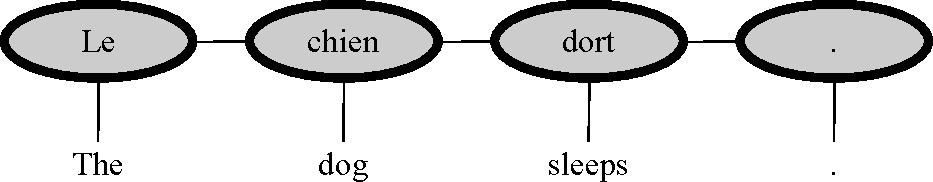
\includegraphics[scale=0.75]{chien}
%\end{center}
%\end{figure}

%\section{The Aim of Research -- Improving the State of the Art}
%
%Like most language technological research, the work documented in this
%thesis aims at improving existing solutions for language
%processing. Specifically, my work is targeted at improving
%morphological taggers for morphologically rich languages. It is not
%entirely easy to define what constitutes an improvement to the field
%of morphological tagging or indeed any sub-field of language
%technology. Nevertheless, most researchers would probably agree that
%the following kinds of changes are improvements compared to existing
%approaches:
%
%\begin{enumerate}
%\item Improving labeling accuracy.
%\item Speeding up estimation.
%\item Speeding up tagging.
%\item Reducing model size. \label{quant}
%\item Clarifying the underlying theoretical foundations.
%\item Simplifying implementation of taggers.
%\item Uncovering best practices for building taggers.
%\end{enumerate}
%
%Items 1 though \ref{quant} in the list above are {\it quantifiable}
%improvements. It is possible to perform experiments to measure the
%labeling accuracy, tagging speed, estimation speed and model size
%given by different morphological taggers and derive conclusions about
%the respective merits of the taggers. In contrast, the rest of the
%items in the list cannot be measured as easily. 
%
%Although, most probably would agree that clarifying theoretical
%foundations of a field is a substantial contribution, it may not be as
%easy to agree upon what constitutes a clarification. This could for
%example be dependent on the background of individual
%researchers. Similarly, one model might be more straight-forward to
%implement than another model using some programming language, however,
%this can very well depend on the specific programming language and
%available libraries to some degree.
%
%Because quantifiable improvements are easier to ascertain, this thesis
%focuses on demonstrating such improvements compared to other state of
%the art approaches. Nevertheless, I will also aim to show that the
%model demonstrated in the thesis is conceptually simpler than other
%state of the art approaches.
%
%Although quantifiable improvements are easier to demonstrate than
%other improvements, there are still caveats. First of all, it is
%impossible to compare machine learning models directly. One can only
%compare implementations of the models. Because of differences between
%platforms even different implementations of the exact same model can
%have radically different run time on the same data. Moreover, bugs in
%the implementation of different models can reduce the accuracy or have
%sporadic effects on run time.
%
%Besides practical concerns like dependence on implementation, there
%are also theoretical issues that interfere with measuring performance
%of different models. It is easy to say that the accuracy of one system
%is better than another system on {\it a specific data set}. This does,
%however, not imply that the accuracy is better on {\it all data
%  sets}. In formal terms, we can only conduct experiments on samples
%of the distribution of all texts in a given language. Therefore, our
%experiments will yield results only in a probabilistic sense: it is
%likely that the labeling accuracy of one system is better than the
%accuracy of another, if the accuracy was better on the sample used for
%testing.
% 
%Using large test sets and test sets compared from a variety of
%different genres will probably give more reliable results. This is,
%however, also to some extent a debatable matter. Some methods are very
%accurate on the same genre that they were trained on but perform worse
%on other genres. Other methods instead perform well on average but, as
%a trade-off, cannot reach as high accuracy on a specific text
%domain. It is not easy to say which kind of system is preferable. This
%trade-off is called the bias variance trade-off \cite{?} and it has
%bearing on measuring the performance difference of systems. 
%
%When using a high variance system, accuracy on different texts varies
%a lot. When instead using a system with high bias, the accuracy tends
%to vary much less.
%
%When comparing two systems, it is not sufficient to simply look at the
%performance of the systems on a test set. If we measure the
%performance of the systems on a particular test, one of them will
%almost certainly perform better than the other regardless of whether
%there is an actual difference in the performances of the systems. The
%probability of exactly equal performance is simply very small. 
%
%The larger the test sets are, the more accurately the results of
%experiments will on average reflect the true performance of the
%systems. This is easy to see, because ultimately the test set will represent the entire domain. Unfortunately, the amount of test material is usually
%restricted and producing more test data might not be
%feasible.\footnote{Especially when using standard data sets, one is
%  restricted to the given amount of test data}
%
%An approach that is often used is splitting the test data into
%segments and performing several experiments -- one for each
%segment. If one system outperforms the other system on most segments
%with a large margin, then we are more confident in saying that there
%is in fact a difference in the performance of the systems. If on the
%hand each system outperforms the other on roughly half of the
%segments, we might be inclined to doubt whether there is any real
%difference in performance between the systems. The higher the variance
%between the results, the larger the margins between the systems need
%to be in order for us to be able to conclude that there is a
%difference in performance. This argument can be made rigorous using
%statistical tests which measure the significance of the difference in
%performance of two systems.
%
%The usual set up of statistical significance testing is to make a null
%hypothesis $H_0$ that the average performance of two systems is the
%same. After this a test statistic is computed. The test statistic is
%simply a real number whose value indicates the significance of the
%difference in performances between the systems. If the statistic is
%high enough, the null hypothesis can be discarded in favor of the
%alternative hypothesis that there is a genuine difference in
%performance between the systems. The test statistic incorporates
%information about the difference in performance of the systems on test
%data all segments as well as the variance of the performances.
%
%In the work conducted presented in this thesis, I have used the
%Wilcoxon signed-rank test \cite{?} to ascertain the significance of
%results. I use it instead of the T-test because it is not dependent on
%the fact that the distribution of differences in performance are
%normally distributed.\footnote{In practice it might be a fairly
%  accurate assumption that the differences are normally
%  distributed. This often holds for measurements \cite{?}.} In
%practice it is less sensitive than the T-test.
%


\chapter{Hidden Markov Models}
\label{chapter:hmm}

AN INTRO

\section{Example}
%\begin{itemize}
%\item Chained stochastic processes \citep{Rabiner1989}.
%\item The three classical problems of HMMs.
%\item Pioneered by \cite{Church1988} in POS tagging.
%\item The results by \cite{Brants2000} and \cite{Halacsy2007} probably
%  represent the generative state of the art.
%\item Very fast to train compared to discriminative models.
%\end{itemize}

I will illustrate Hidden Markov Models using an example. Imagine a
person called Jill who is hospitalized and occupies a windowless
room. The only way for her to know what is happening in the outside
world is to observe a nurse who passes her room daily\footnote{To make things simple, imagine the nurse never gets a day
  off.}.

Suppose, Jill is interested in weather phenomena and she decides to
pass time by guessing if it is raining outside. She bases her guesses
on whether or not the nurse is carrying an umbrella. In other words,
she predicts an unobserved variable, the weather, based on an observed
variable, the nurse's umbrella.

There are several probabilistic models Jill might use. The simplest
useful model assigns probability $1$ to the event of rain, if the
nurse carries an umbrella, and assign it the probability $0$
otherwise. This simplistic model would certainly give the correct
prediction most of the time, but Jill believes that she can do better.

Jill knows that people often carry an umbrella when it is raining. She
also knows that they rarely carry one when the weather is
clear. However, people sometimes do forget their umbrella on
rainy days, perhaps because they are in a hurry. Moreover, people
sometimes carry an umbrella even when it is not raining. For example
the weather might be murky and they might anticipate rain. Therefore,
Jill decides to reserve some probability, say $0.2$, for the event
that the nurse is carrying an umbrella when the weather is clear. She
reserves an equal probability for the event that the nurse arrives at
work without an umbrella although it is in fact raining.
 
Without additional information, this more complicated model will give
exactly the same MAP predictions as the simplistic one. Knowledge of
meteorology, however, also factors in. Let us suppose Jill is a
weather enthusiast and she knows that the probability of rain is
$0.25$ a priori, making the probability of clear weather $0.75$. She also knows
that the probability of rain increases markedly on days following
rainy days at which time it is $0.7$.  Similarly, the probability of
clear weather increases to $0.9$ if the weather was clear on the
previous day. Figure \ref{hmm-ex-1} summarizes these
probabilities.\footnote{Since the author of this thesis has very
  little knowledge about meteorology, these probabilities are likely
  to be nonsense. The overall probability of rain and clear weather
  is, however, chosen to be the steady state of the Markov chain
  determined by the probabilities of transitioning between
  states. Consistency is therefore maintained.}

\begin{figure}[!htb]
\begin{center}
\begin{tabular}{|l|c|}
\hline
   $\iota$   &       \\
\hline
CLEAR  & $0.75$ \\
RAIN  & $0.25$ \\
\hline
\end{tabular}~~~
\begin{tabular}{|l|cc|}
\hline
   $T$   & CLEAR & RAIN  \\
\hline
CLEAR  & $0.9$ & $0.1$ \\
RAIN   & $0.3$ & $0.7$ \\
\hline
\end{tabular}~~~
\begin{tabular}{|l|cc|}
\hline
   $E$   & 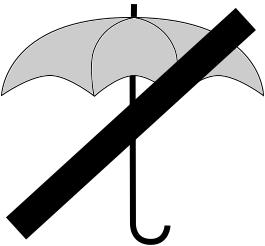
\includegraphics[width=0.5cm]{no_umbrella} & 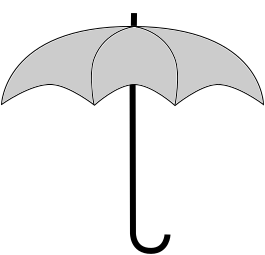
\includegraphics[width=0.5cm]{umbrella} \\
\hline
CLEAR   & $0.8$ &  $0.2$         \\
RAIN    & $0.2$ &  $0.8$         \\
\hline
\end{tabular}
\end{center}
\caption{Foo FIXME}\label{hmm-ex-1}
\end{figure}

Let us assume that Jill observes the nurse for one week. She sees the
nurse carry an umbrella on all days except Tuesday. The MAP prediction
given by the simplistic model is that Tuesday is clear and all other
days are rainy. The more complex model will, however, give a different
MAP prediction: the probability is maximized by assuming that all days
are rainy. Under the more complex model, it is simply more likely that
the nurse forgot to bring an umbrella on Tuesday.

\begin{figure}[!htb]
\begin{center}
\caption{Foo}\label{hmm-ex-2}
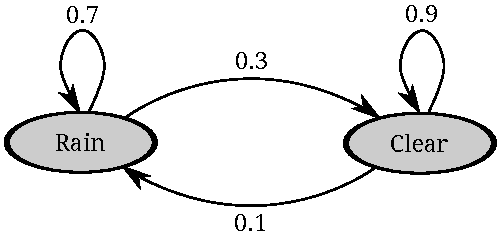
\includegraphics[scale=0.8]{hmm-ex-graph}
\end{center}
\end{figure}

The model Jill is using for weather prediction is called a Hidden
Markov Model. It can be used to make predictions about a series of
events based on indirect observations. 

The HMM is commonly visualized as a directed graph. Each hidden state,
for example Rain and Clear, represents a vertex in the
graph. Transitions from one hidden state to another are represented by
arrows labeled with probabilities. Figure \ref{hmm-ex-2} shows a graph
representing the transition structure of the HMM outlined in Figure
\ref{hmm-ex-1}.

\section{Formal Definition}

%\begin{itemize}
%\item Model derivation.
%\item Lexical model.
%\item First order transition model.
%\item Model order.
%\item Guesser for OOV words à la Brants.
%\end{itemize}

Abstracting from the example above, an HMM is a probabilistic model
that generates sequences of state-observation pairs. At each step $t$
in the generation process, the model generates an observation by
sampling the {\it emission distribution} $\varepsilon_{y_t}$ of the
current state $y_t$. It will then generate a successor state $y_{t+1}$
by sampling the {\it transition distribution} $\tau_{y_t}$ of state
$y_t$. The first hidden state $y_1$ is sampled from the {\it initial
  distribution} $\iota$ of the HMM.

Since the succession of days is infinite for all practical purposes,
there was no need to consider termination in the example presented in
Figure \ref{hmm-ex-2}. Nevertheless, many processes, such as sentences, do
have finite duration. Therefore, a special {\it final state} $f$ is
required. When the process arrives at the final state, it stops:
no observations or successor states are generated.

Following \cite{Rabiner1989}, I formally define a {\it discrete} HMM as a
structure $(Y,\ X,\ i,\ T,\ E,\ F)$ where:
\begin{enumerate}
\item $Y$ is the set of hidden states ($Y = \{{\rm CLEAR},$ ${\rm RAIN}\}$
  in the example in Figure \ref{hmm-ex-1}).
\item $X$ is the set of emissions, also called observations (
%$\Sigma =
%  \{{\rm Umbrella},$ ${\rm No\ umbrella}\}$ 
$X = \{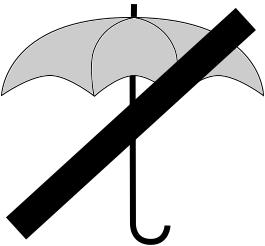
\includegraphics[width=0.4cm]{no_umbrella},\ 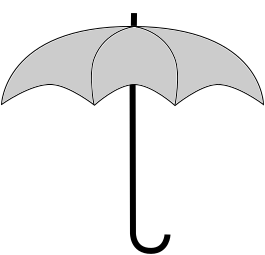
\includegraphics[width=0.4cm]{umbrella}\}$
in the example in Figure
  \ref{hmm-ex-1}).
\item $\iota: Y \rightarrow \R$ is the initial state distribution, that is the probability
  distribution determining the initial state of an HMM process (array
  $\iota$ in Figure \ref{hmm-ex-1}).
\item $T$ is the collection of transition distributions, $\tau_y: Y \rightarrow \R$, that
  determine the probability of transitioning from a state $y$ to each state
  $y' \in Y$ (array $T$ in Figure \ref{hmm-ex-1}).
\item $E$ is the collection of emission distributions $\varepsilon_y:
  X \rightarrow \R$, which determine the probability of observing each
  emission $o \in X$ in state $y \in Y$ (array $E$ in Figure
  \ref{hmm-ex-1}).
\item $f \in Y$ is the final state. The state $f$ emits no
  observations and there are no transitions from $f$.
\end{enumerate}
The definition of HMMs in this thesis differs slightly from
\cite{Rabiner1989} since I utilize final states. Final states were
used in for example \cite{foo}. Absorbing states \cite{bar} could also
be used. FIXME.

Figure \ref{hmm-ex-3} is a more accurate description of the HMM in
Figure \ref{hmm-ex-1} than Figure \ref{hmm-ex-2}. The image has been
augmented with initial distribution and a final state. 

Because the progression of days is infinite for all practical purposes, the
probability of transitioning to the final state $f$ in example
\ref{hmm-ex-2} is 0 regardless of the current state. Hence, the
probability of any single sequence of states and emissions is
0. Still, the probability of an initial segment of a state sequence
may still be non-zero\footnote{The probability of an initial segment
  up to position $t$ can be computed using the forward algorithm,
  which is presented in Section \ref{sec:forward}.}.% For example, the
%probability that the first three states are (RAIN, RAIN, CLEAR) is X.

\begin{figure}[!htb]
\begin{center}
\caption{Foo}\label{hmm-ex-3}
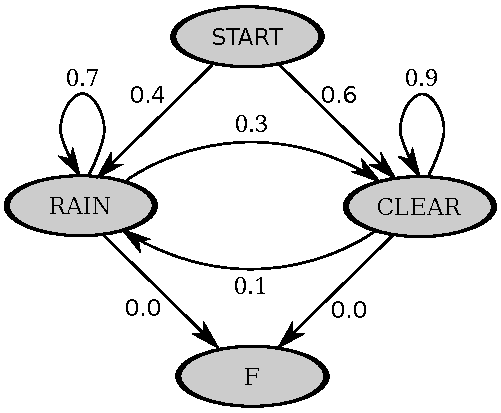
\includegraphics[scale=0.8]{hmm-ex-graph-2}
\end{center}
\end{figure}

An HMM models a number of useful quantities:
\begin{enumerate}
\item The {\it joint probability} $p(x,y\parcond\theta)$ of a observation
  sequence $x$ and state sequence $y$. This is the probability that an
  HMM with parameters $\theta$ will generate the state sequence $y$
  and generate the observation $x_t$ in every state $y_t$.
\item The {\it marginal probability} $p(x\parcond \theta)$ of an
  observation sequence $x$. This is the overall probability that the
  observation sequence generated by an HMM is $x$.
\item The {\it conditional probability} $p(y\cond x\parcond\theta)$ of a
  state sequence $y$ given an observation sequence $x$. That is, how
  likely it is that the model passes through the states in $y$ when
  emitting the observations in $x$ in order.
\item The {\it marginal probability $p(z, t,\ x\parcond \theta)$ of
    state $z$ at position $t$} when emitting the observation sequence
  $x$. That is, the probability of emitting observation sequence $x$
  under the single constraint that the state at position $t$ has to be $z$.
\end{enumerate}

To formally define these probabilities, let $\theta = \{\iota,\ T,\
E\}$ be the parameters of some HMM with observation set $X$ and hidden
state set $Y$, $x = (x_1,\ ...,\ x_T) \in X^T$ be a sequence of
observations and $y = (y_1,\ ...,\ y_T, y_{t+1} = f) \in Y^{T+1}$ a sequence of
hidden states. Note, that the last state in $y$ has to be the final state
$f$. Then the joint probability $p(x,y\parcond\theta)$ of $x$ and $y$
given $\theta$ is defined by Equation \eqref{hmm-joint-prob}.
\begin{equation}
p(x,y\parcond\theta) = p(y\parcond\theta)\cdot p(x \cond y\parcond\theta)= \Bigg(\iota(y_1) \cdot \prod_{t = 1}^{T} \tau_{y_t}(y_{t + 1})\Bigg) \cdot \prod_{t = 1}^T \varepsilon_{y_t}(x_t)\label{hmm-joint-prob}
\end{equation}
Equation \eqref{hmm-joint-prob} is a product of two factors: the
probability of the hidden state sequence $y$, determined by the
initial and transition probabilities, and the probability of the
emissions $x_t$ given hidden states $y_t$ determined by the emission
probabilities.

FIXME: Talk about language models and stuff.

There is no limit on the number of hidden states in $Y$ that can emit
a given observation. Therefore, it is quite possible that several
state sequence $y \in Y^{T+1}$ can be generate the same sequence of observations
$x \in X^T$. The marginal probability $p(x\parcond\theta)$ of an observation
sequence $x$ can be found by summing over all state sequences that
could have generated $x$. It is defined by Equation
\eqref{hmm-obs-prob}.
\begin{equation}
p(x\parcond\theta) = \sum_{y \in Y^{T+1},\ y_{T+1} = f} p(x, y\parcond \theta)\label{hmm-obs-prob}
\end{equation}

Possibly the most important probability associated to the HMM is the
conditional probability $p(y\cond x\parcond\theta)$ of state sequence $y$
given observations $x$. This is an important quantity because
maximizing $p(y\cond x\parcond\theta)$ with regard to $y$ will give the MAP
assignment of observation sequence $x$. It is defined by Equation
\eqref{hmm-cond-prob}.
\begin{equation}
p(y\cond x\parcond\theta) = \frac{p(x,y\parcond\theta)}{p(x\parcond\theta)}\label{hmm-cond-prob}
\end{equation}
It is noteworthy, that $p(y\cond x\parcond\theta) \propto p(x,y\parcond\theta)$ because the marginal probability $p(x\parcond\theta)$ is independent of $y$. Therefore, $y$ maximizes $p(y\cond x\parcond\theta)$ if and only if, it maximizes $p(x,y\parcond\theta)$. This facilitates inference.

Finally, the posterior marginal probability of state $z$ at position $t$ given
the observation sequence $x$ is computed by summing, or marginalizing,
over all state sequence $y$, where $y_t = z$. It is defined by
Equation \eqref{hmm-marg-prob}
\begin{equation}
p(z, t,\ x\parcond \theta) = \sum_{y' \in Y^{T+1},\ y'_t = z,\ y'_{T+1} = f} p(x, y'\parcond \theta)\label{hmm-marg-prob}
\end{equation}

\section{Inference}
%\begin{itemize}
%\item The forward algorithm.
%\item Guarding against underflow: Dynamic scaling \citep{Rabiner1989} or exp-sum-log \citep{Durbin1998}.
%\item The Viterbi algorithm.
%\item Fixed beam search.
%\item Determining the beam: fixed, threshold and adaptive beam \citep{pal2006}.
%\item The forward-backward algorithm and multitagging.
%\end{itemize}
Informally, inference in HMMs means finding a maximally
probable sequence of hidden states $y$ that might have emitted the
observation $x$. As \cite{Rabiner1989} points out, this statement is
not strong enough to suggest an algorithm. 

Maximally probable is an ambiguous term when dealing with structured
models. It could be taken to mean at least two distinct things. The
MAP assignment $y_{MAP}$ of the hidden state sequence is the most
probable joint assignment of states defined by Equation
\eqref{hmm-map} and depicted in Figure
\ref{hmm-ex-trellis-path}. 
\begin{equation}
y_{MAP} = \argmax_{y\in Y^T} p(y\cond x\parcond\theta)\label{hmm-map}
\end{equation}

Another possible definition would be the
{\it maximum marginal} (MM) assignment. It chooses the most probable
hidden state for each word considering all possible assignments of states for the remaining words. The MM assignment $y_{MM}$ is defined by Equation
\eqref{hmm-mm}. Figure \ref{hmm-ex-trellis-marginal} shows the
marginal for one position and state.


\begin{equation}
y_{MM} = \argmax_{y\in Y^T} \prod_{t = 1}^T p(y_t, t \cond x\parcond\theta)\label{hmm-mm}
\end{equation}

As \cite{Merialdo1994} and many others have noted, the MAP and MM
assignments maximize different objectives. The MM assignment maximizes
the accuracy of correct states per observations whereas the MAP
assignment maximizes the number of completely correct state
sequences. Both objectives are important from the point of view of POS
tagging. However, they are often quite correlated and, at least in POS
tagging, it does not matter in practice which of the criteria is used
\citep{Merialdo1994}. Most systems, for example
\cite{Church1988,Brants2000,Halacsy2007}, have chosen to use MAP
inference.

Although, MM inference is more rarely used with HMMs, computing the
marginals is important both in unsupervised estimation of HMMs and
discriminative estimation of sequence models. Therefore, an efficient
algorithm for MM inference, the {\it forward algorithm}, is presented below.

There are a number of strongly related algorithms for both exact MAP
and MM inference. The work presented in this thesis, uses the Viterbi
algorithm for MAP inference and the forward-backward algorithm for MM
inference \citep{Rabiner1989}. {\it Belief propagation}, introduced by
\cite{Pearl1982}, computes the MM assignment and can be modified to
compute the MAP assignment as well. For sequence models, such as the
HMM where hidden states form a directed sequence, belief propagation
is very similar to the forward-backward algorithm. It can, however, be
extended to cyclic graphs \citep{Weiss2000} unlike the Viterbi
algorithm.

Since cyclic models fall beyond the scope of this thesis and both the
Viterbi and forward-backward algorithms are amenable to well known
optimizations, which are of great practical importance, I will not
discuss belief propagation belief propagation
further. \cite{Koller2009} gives a nice treatment of belief
propagation and graphical models at large.

Before introducing the Viterbi and forward-backward algorithm, it is
necessary to investigate the forward algorithm, which is used to
compute the marginal probability of an observation and also as part of
the forward-backward algorithm. The forward algorithm and Viterbi
algorithm are closely related.

\begin{figure}[!p]
\begin{center}
\caption{foo.}\label{hmm-trellis}
\begin{subfigure}{\textwidth}
\begin{center}
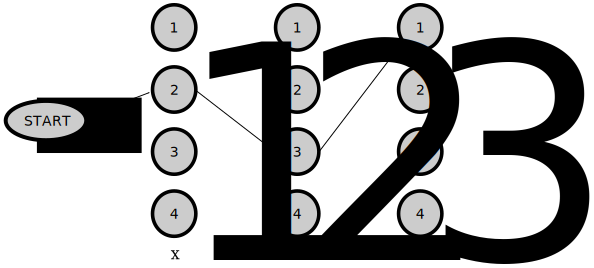
\includegraphics[scale=0.65]{trellis_path}
\caption{Trellis and path.}\label{hmm-ex-trellis-path}
\end{center}
\end{subfigure}
\vskip.5cm
\begin{subfigure}{\textwidth}
\begin{center}
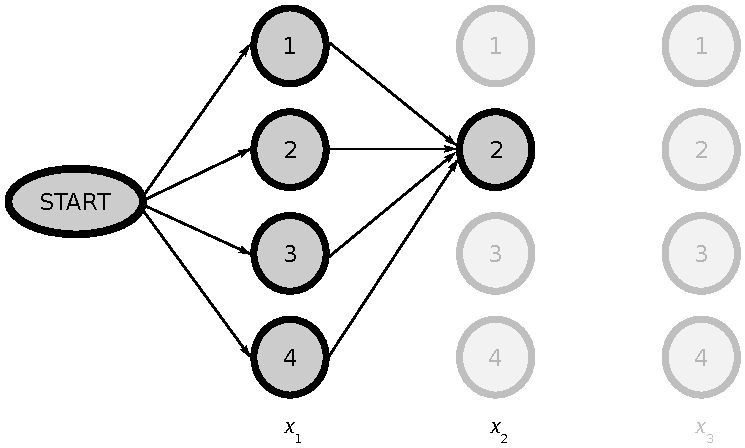
\includegraphics[scale=0.65]{trellis_forward}
\end{center}
\caption{Forward path prefixes.}\label{hmm-ex-trellis-fw}
\end{subfigure}
\vskip.5cm
\begin{subfigure}{\textwidth}
\begin{center}
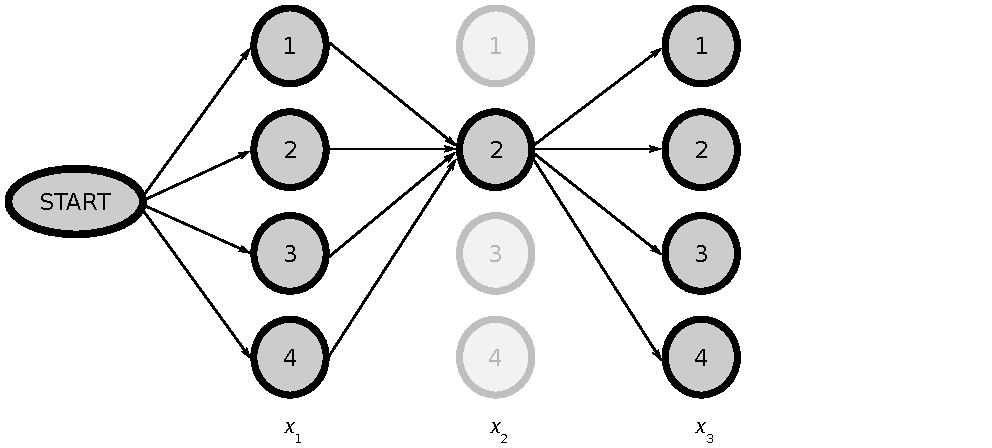
\includegraphics[scale=0.65]{trellis_marginal}
\end{center}
\caption{Marginal paths.}\label{hmm-ex-trellis-marginal}
\end{subfigure}
\end{center}
\end{figure}

\subsection{The Forward Algorithm}
\label{sec:forward}
Equations \eqref{hmm-map} and \eqref{hmm-mm} reveal, that both MAP
and MM inference require knowledge of the entire observation $x$. In
the weather prediction example, observations are, however, always
infinite. What kind of inference is possible in this case?

Even when we only know a prefix $x[1:t]$ (of length $t$) of the entire
observation $x$, we can still compute the {\it belief state}
\citep{Boyen1998} of the HMM given the prefix. The belief state is in
fact not a single state, but rather a distribution over the set of
hidden states $Y$. It tells us how likely we are to be in state $z$ at
time $t$, when we have emitted the prefix $x[1:t]$.

To compute the belief state at position $t$, we first need to compute
the {\it forward probabilities} for each state $z \in Y$. The forward
probability $\fw_{t,z}(x)$ of state $z$ at position $t$ is the
probability of emitting prefix $x[1:t]$ and ending up in state $z \in
Y$. For example, given an infinite observation 
%$x = (${\sc umbrella},
%{\sc umbrella}, {\sc no umbrella},\ ...$)$
$\{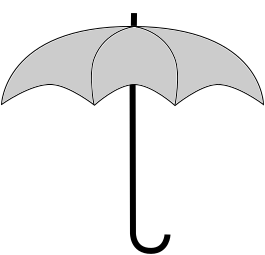
\includegraphics[width=0.4cm]{umbrella},\ 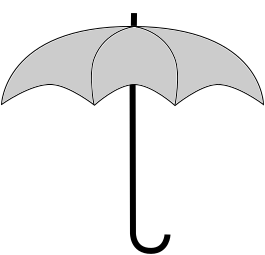
\includegraphics[width=0.4cm]{umbrella},\ 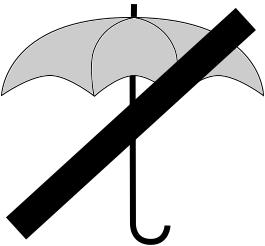
\includegraphics[width=0.4cm]{no_umbrella},\ ...\}$, the forward probability
$\fw_{3,\textsc{RAIN}}$ is the probability that the third day is rainy,
when the nurse carried an umbrella on the first and second days, but
did not carry one on the third day.

I am going to make a technical but useful definition. The {\it prefix probability} of observation sequence $x = (x_1,\ ...,\ x_T)$ and state sequence $y = (y_1,\ ...,\ y_t)$ at position, where $t < T + 1$ is given by Equation \eqref{prefix_prob}. 
\begin{equation}
p(x,\ y\parcond \theta) = \Bigg(\iota(y_1) \cdot \Bigg(\prod_{u = 1}^{t - 1} \tau_{y_u}(y_{u + 1}) \Bigg) \cdot \prod_{u = 1}^t \varepsilon_{y_u}(x_u)\Bigg),\ t \le T\label{prefix_prob}
\end{equation}
When $t = T$, this is very similar to the joint probability of $x$ and
$y$, but the final transition is missing.

Conceptually, the forward probability is computed by summing over the
probabilities of all path prefixes up to position $t$, where the state
at position $t$ is $z$, see Figure \ref{hmm-ex-trellis-fw}. Formally,
the forward probability is defined by Equation \eqref{forward_prob}.
\begin{equation}
\fw_{t,z} = \sum_{y\in Y^t,\ y_t = z} p(x,\ y\parcond\theta)\label{forward_prob}
\end{equation}
Comparing Equations \eqref{forward_prob} and \eqref{hmm-joint-prob}
shows that the forward probability in a sense represents the
probability of a prefix of observation $x$.

The belief state and posterior marginal distribution may seem
similar. They are, however, distinct distributions because the belief
state disregards all information about observation $x$ after position
$t$. In contrast, the marginal distribution encompasses information
about the entire observation. For example the marginal probability of
RAIN at position 3 is likely to depend strongly on whether or not Jill
observes the nurse carry an umbrella on the fourth day. However, this
will have no impact on the belief state.

Figure \ref{fw-naive-prob} demonstrates a naive approach to computing
the forward probabilities. Simply list all relevant state sequences,
compute the probability of each sequence and sum the
probabilities. Unfortunately, the naive approach fails for large $t$
because the number of distinct state sequences depends on the sequence
length in an exponential manner.

The complexity of the naive algorithm is $|Y|^t$, which is infeasible.
For example, $f_{20,\textsc{RAIN}}(x)$ requires us to sum
approximately 20 million probabilities and $f_{30,\textsc{RAIN}}(x)$
entails summation of approximately 540 million probabilities. Since
observation sequences in domains such as natural language processing
frequently reach lengths of $100$, a more efficient approach is required.

\begin{figure}[!ftb]
\begin{center}
\caption{foo}\label{fw-naive-prob}
\begin{tabular}{lllr}
$y_1$ & $y_2$ & $y_3$ & $p$ \\
\hline
{\sc CLEAR} & {\sc CLEAR} & {\sc CLEAR} & $(0.75\cdot0.8\cdot0.9\cdot0.2)\cdot0.9\cdot0.8\approx0.078$\\
{\sc RAIN}  & {\sc CLEAR} & {\sc CLEAR} & $(0.25\cdot0.2\cdot0.3\cdot0.2)\cdot0.9\cdot0.8\approx0.002$\\
{\sc CLEAR} & {\sc RAIN}  & {\sc CLEAR} & $(0.75\cdot0.8\cdot0.1\cdot0.8)\cdot0.3\cdot0.8\approx0.012$\\
{\sc RAIN}  & {\sc RAIN}  & {\sc CLEAR} & $(0.25\cdot0.2\cdot0.7\cdot0.8)\cdot0.3\cdot0.8\approx0.007$\\
& & & \\
%\hline
%\vspace{0.1cm}
~~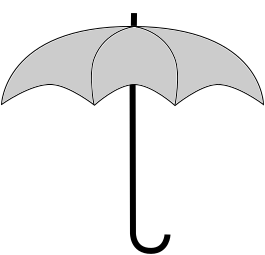
\includegraphics[width=0.5cm]{umbrella} & ~~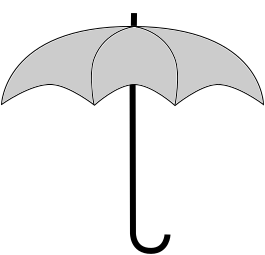
\includegraphics[width=0.5cm]{umbrella} & ~~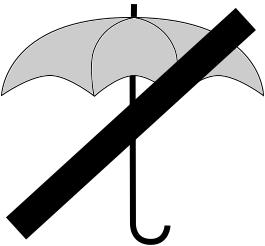
\includegraphics[width=0.5cm]{no_umbrella} & \\
\hline
        &       & & $\approx0.098$
\end{tabular}
\end{center}
\end{figure}

The belief state can be computed in linear time with regard to $t$ and
quadratic time with regard to $|Y|$ using the {\it forward algorithm}
\citep{Rabiner1989}, which is in fact simply a recursive application
of the right distributive rule of algebra
$$a_1 \cdot b + ... + a_n \cdot b = (a_1 + ... + a_n)\cdot b$$
for real numbers $a_1$ up to $a_n$ and $b$. 

Instead of computing the probability separately for each path, the
forward probabilities for longer paths are computed incrementally
using the forward probabilities of shorter paths. Examine Figure
\ref{fw-naive-prob}. By grouping rows one and two, as well as three
and four into pairs, it is easy to see that
$$\fw_{3,\textsc{CLEAR}} = (\fw_{2, \textsc{RAIN}}\cdot \tau_{\textsc{RAIN}}(\textsc{CLEAR}) + \fw_{2, \textsc{CLEAR}} \cdot \tau_{\textsc{CLEAR}}(\textsc{CLEAR})) \cdot \varepsilon_{\textsc{CLEAR}}(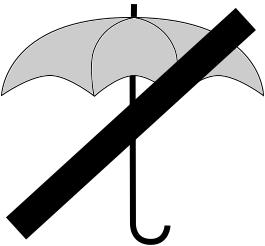
\includegraphics[width=0.4cm]{no_umbrella})$$
Generalizing, we get the recursion in Equation \eqref{fw-rec}.
\begin{equation}
\fw_{t, z} = \left\{
\begin{aligned}
&\iota(z) \cdot \varepsilon_{z}(x_1)  & , &\  t = 1\\
&\Bigg(\sum_{z'\in Y} \fw_{t - 1, z'}\cdot \tau_{z'}(z) \Bigg) \cdot \varepsilon_{z}(x_{t}) & ,&\ 1 < t \le T\\
&\sum_{z'\in Y} \fw_{T, z'}\cdot \tau_{z'}(f) & ,&\  t = T + 1,\ z = f.
\end{aligned}
\right.
\label{fw-rec}\end{equation}
The remaining forward probabilities $\fw_{T+1, z}$, where $z \ne f$
are defined to be $0$.

The forward probability $f_{T + 1, f} = p(x \parcond \theta)$. In fact
one of the principal applications for the forward algorithm is
computing the marginal probability of an observation. The other
central application is in the forward-backward algorithm, which
computes the state marginals.
  
The forward algorithm is outlined in Algorithm
\ref{forward-algorithm}. Assuming that accessing the data structures
{\tt x}, {\tt i_prob}, {\tt e_prob}, {\tt tr_prob} and {\tt trellis}
is constant time, the complexity of the algorithm is dominated by the
three nested loops on lines \ref{start-cplx}--\ref{stop-cplx}. This
shows that the complexity of the forward algorithm is linear with
regard to the length of the sequence and quadratic with regard to the
size of the hidden state set.

Although, the forward algorithm depends linearly on the observation
length, its quad\-ra\-tic dependence on the size of the hidden state set
is problematic from the perspective of morphological disambiguation of
morphologically complex languages, where the size of the hidden state
set is measured in the hundreds or thousands for regular HMMs. When
using second order HMMs presented below, the state set can grow to
tens of thousands or millions, which can slow down systems to a degree
that makes them infeasible in practice. I will present partial
solutions to these problems below.

\begin{algorithm}[!p]
\begin{center}
\caption{The forward algorithm in Python 3.}\label{forward-algorithm}
\begin{lstlisting}[linewidth=\textwidth]
def forward(x, i_prob, e_prob, tr_prob): 
    """
        x       - The observation as a list.
        i_prob  - Initial state distribution.
        e_prob  - Emission distributions.
        tr_prob - Transition distributions.

        Return the trellis of forward probabilities. 
    """

    assert(not x.empty()) 

    trellis = {}

    # Indexing in python starts at 0.
    x_1 = x[0]
    T   = len(x) + 1

    # Set final state F. States are consequtive integers 
    # in the range [0, F]. 
    F = len(i_prob) - 1 

    # Initialize first trellis column.
    for z in range(F):
        trellis[(1,z)] = i_prob[z] * e_prob[z][x_1]

    # Set all except the final column.(*@\label{start-cplx}@*)
    for t in range(2, T):
        trellis[(t, z)] = 0

        x_t = x[t - 1]

        for z in range(F):
            for s in range(F):
                trellis[(t, z)] = trellis[(t - 1, s)] * tr_prob[s][z]

            trellis[(t, z)] *= em_prob[z][x_t](*@\label{stop-cplx}@*)

    # Set the last column.
    for z in range(s_count):
        trellis[(T + 1, z)] = trellis[(T, z)] * tr_prob[z][F]

    return trellis 
\end{lstlisting}
\end{center}
\end{algorithm}

\subsection{The Viterbi Algorithm}
\label{hmm-viterbi}

Whereas the forward algorithm incrementally computes the marginal
probability of an observation $x$, the Viterbi algorithm incrementally
computes the MAP assignment for observation $x$.

A naive approach to finding the MAP assignment is to list all the
hidden state paths, compute their probabilities and pick the one with
the highest probability. Similarly as for the forward algorithm, the
complexity of this approach is exponential with regard to the length
of observation $x$.

Just as in the case of forward probabilities, the MAP assignment of
hidden states for a prefix of the observation $x$ can be computed
incrementally. Formally, the MAP assignment for a prefix $x[1:t]$ is
defined by equation \eqref{map_prefix} utilizing the joint prefix
probability of $x$ and a state sequence $y$ of length
$t$. Intuitively, it is the sequence of hidden states $y_{t, z}$ which
maximizes the joint probability and ends at state $z$.
\begin{equation}
y_{t,z} = \argmax_{y\in Y^t,\ y_t = z} p(x,\ y\parcond \theta)\label{map_prefix}
\end{equation}
Comparing this equation with the definition of the forward probability
$f_{t,z}$ in Equation \ref{forward_prob}, we can see that the only
difference is that the sum has been changed to $\argmax$.

I will now show that the MAP prefix $y_{t,z}$ can be computed
incrementally in a similar fashion as the forward probability
$f_{t,z}$. Suppose that $y_{t+1, z'} = (y_1,\ ...,\ y_t = z,\ y_{t+1}
= z')$. I will show that $y_{t+1, z'}[1:t] = y_{t,z}$. Let $y'$ be the concatenation of $y_{t,z}$ and $z'$. If $y_{t+1,z'}[1:t] \ne y_{t,z}$, then
\begin{eqnarray*}
p(x,\ y_{t+1,z'}\parcond \theta) & = & p(x,\ y_{t+1,z'}[1:t]\parcond \theta) \cdot \tau_z(z')\cdot\varepsilon_{z'}(x_{t+1})\\ 
                                 & < & p(x,\ y_{t,z}\parcond \theta) \cdot \tau_z(z')\cdot\varepsilon_{z'}(x_{t+1})\\
                                 & = & p(x, y'\parcond\theta)
\end{eqnarray*}
This contradicts the definition in Equation \eqref{map_prefix}\footnote{As long as we suppose that there is exactly one MAP prefix.}.

We now get Equation \eqref{map-rec}, which gives us a recursion.
\begin{equation}
y_{t+1, z} = \argmax_{z \in Y}\left\{
\begin{aligned}
&\iota(z) \cdot \varepsilon_{z}(x_1)  & , &\  t = 1\\
&y_{t - 1, z'}\cdot \tau_{z'}(z) \cdot \varepsilon_{z}(x_{t}) & ,&\ 1 < t \le T\\
&y_{T, z'}\cdot \tau_{z'}(f) & ,&\  t = T + 1,\ z = f.
\end{aligned}
\right.
\label{map-rec}
\end{equation}

\subsection{Beam Search}

As seen in the previous section, the complexity of the Viterbi
algorithm depends on the square of the size of the hidden state
set. This can be problematic when the set of hidden states is large,
for example when the states represent POS tags in a very large label
set or when they represent combinations of POS tags. When tagging, a
morphologically complex language, the state set may easily encompass
hundreds or even thousands of states.

{\it Beam search} is is a heuristic which prunes the search space
explored by the Viterbi algorithm based on the following observation:
in many practical applications, the number of hidden states which emit
a given observation with appreciable probability is small. This is
true even when the total number of hidden states is very large. For
example, when the states represent POS labels, a given word such as
``dog'' can usually only be emitted by a couple of states (maybe Noun
and Verb in this case).

When the Viterbi algorithm maximizes \eqref{map-rec} for $y_{t+1,z}$,
a large number of histories $y_{t,z}$ can, therefore, be ignored.

Often a constant number, the {\it beam width}, of potential histories
are considered in the maximization. The complexity of the Viterbi
algorithm with beam search is $o(|Y|\cdot \log|Y|)$. The log factor
stems from the fact that the histories need to be sorted before
maximization.\footnote{Sequential decoding, an approximate inference
  algorithm, which was used for decoding before the Viterbi algorithm
  was in common use \citep{Forney2005} is very similar to beam
  search. Indeed, it could be said that Viterbi invented an exact
  inference algorithm, which is once more broken by beam search.}

In addition to histories, the possible hidden states for output can
also be filtered. The simplest method in to use a so called tag
dictionary. These techniques are described in Section
\ref{sec:hmm-label-dict}.

\subsection{The Forward-Backward Algorithm}
\label{hmm-fw-bw}
The Viterbi algorithm computes the MAP assignment for the hidden
states efficiently. For efficiently computing the marginal probability
for a every state and position (see Figure
\ref{hmm-ex-trellis-marginal}), the forward-backward algorithm is
required.

Intuitively, the probability that a state sequence $y$ has state $z \in Y$
at position $t$, that is the probability that $y_t = z$ is the product
of the probabilities that the prefix $y[1:t]$ ends up at state $z$ and
the probability that the suffix $y[t:T]$ originates at $z$. 

The name forward-backward algorithm stems from the fact, that the
algorithm essentially consists of one pass of the forward algorithm,
which computes prefix probabilities, and another pass of the forward
algorithm starting at the end of the sentence and moving towards the
beginning which computes suffix probabilities. Finally, the forward
and suffix probabilities are combined to give the marginal probability
of all paths where the state at position $t$ is $z$. These passes are
called the forward and backward pass.

Formally, the suffix probabilities computed by the backward pass are
defined by equation \eqref{bw-rec}.

Since a backward pass of the forward algorithm carries the same
complexity as the forward pass, we can see that the complexity of the
forward-backward algorithm is the same as the complexity of the
forward algorithm, however, there is a constant factor of two compared
to the forward algorithm.

\begin{equation}
b_{t, z} = \left\{
\begin{aligned}
&\Bigg(\sum_{z'\in Y}t_{z}(z') \cdot  b_{t + 1, z'} \Bigg) \cdot e_{z}(x_{t+1}) & ,&\ 1 < t < T\\
&t_{z}(f) & ,&\  t = T + 1,\ z = f.
\end{aligned}
\right.
\label{bw-rec}
\end{equation}

\subsection{Sparse Forward-Backward Algorithms}

FIXME \citep{Pal2006}.

\section{Estimation}
%\begin{itemize}
%\item Counting vs Baum-Welch.
%\item Smoothing over orders.
%\item Smoothing missing counts.
%\item Estimating parameters for OOV word model.
%\end{itemize}

HMMs can be trained in different ways depending on the quality of the
available data, but also on the task at hand. The classical setting
presented by \cite{Rabiner1989} is nearly completely unsupervised: the
HMM is trained exclusively from observations. Some supervision is
nevertheless usually required to determine the number of hidden
states\footnote{Although methods for determining the number of states
  from the data exist \citep{foo}.}. Additionally priors on the
emission and transitions distributions may be required to avoid
undesirably even distributions
\citep{Cutting1992,Johnson2007}.

The unsupervised training setting has two important and
interrelated applications:
\begin{enumerate}
\item Modeling a complex stochastic process from limited data. Here
  the HMM can be contrasted to a Markov chain \citep[318--320]{Manning1999}, where
  each emission can occur in a unique state leading to a higher degree
  of data sparsity and inability to model under-lying structure.
\item Uncovering structure in data, for example part-of-speech
  induction \citep{Johnson2007}.
\end{enumerate}
The classical method for unsupervised Maximum likelihood estimation of
HMMs is the {\it Baum-Welch algorithm} \citep{Rabiner1989}, which is
an instance of the {\it expectation maximization algorithm} (EM)
\citep{Dempster1977} for HMMs.

In POS tagging and morphological disambiguation, the supervised
training scenario is normally used. Supervised training consists of
annotating a text corpus with POS labels and estimating the emission
and transition probabilities from the annotated data. 

Straight-forward counting is sufficient to get the ML estimates for
the transition and emission distributions. For example, one can simply
count how often a determiner is followed by a noun, an adjective or
some other class. Similarly, one can count how many often a verb label
emits ``dog'' and how often the noun label emits ``dog''. 

Even in large training corpora, ``dog'' might very well never receive
a verb label\footnote{There are ten occurrences of ``dog'' in the Penn
  Treebank and all of them are analyzed as nouns.}. Nevertheless,
``dog'' can be a verb, for example in the sentence ``Fans may dog
Muschamp, but one thing's for certain: he did things the right way off
the field.''. To avoid this kind of problems caused by data sparsity,
both emission and transition counts need to be smoothed.

\subsection{Counting for Supervised ML Estimation}

When HMMs are used in linguistic labeling tasks, such as
part-of-speech tagging, they are usually estimated in a supervised
manner. Each label is thought to represent a hidden variable, and the
HMM models the transitions from one label type to another and the
emission of words from each label type. 

\begin{figure}[!htb]
\begin{center}
\begin{BVerbatim}
Mr.             NNP
Vinken          NNP
is              VBZ
chairman        NN
of              IN
Elsevier        NNP
N.V.            NNP
,               ,
the             DT
Dutch           NNP
publishing      VBG
group           NN
.               .
\end{BVerbatim}
\end{center}
\caption{foo}\label{penn-figure}
\end{figure}

Figure \ref{penn-figure} shows one sentence from the Penn Treebank \citep{Marcus1993}. The sentence is labeled with POS tags which are taken to be the hidden states of an HMM. When estimating an HMM tagger for the corpus, transitions probabilities, for example $t_{{\tt NNP}, {\tt VBZ}}$, and emission probabilities, for example $e_{{\tt NNP}}({\tt Dutch})$ can in principle be computed directly from the corpus. For example the transition probability $t_{{\tt NNP}, {\tt VBZ}}$ and the emission probability $e_{{\tt NNP}}({\tt Dutch})$ in the Penn Treebank are simply:
$$t_{{\tt NNP}, {\tt VBZ}} = \frac{{\rm Count\ of\ POS\ tag\ pair\ {\tt NNP}\ {\tt VBZ}\ in\ the\ corpus}}{{\rm Count\ of\ POS\ tag\ {\tt NNP}\ in\ the\ corpus}} = \frac{4294}{114053} \approx 0.04$$

$$e_{{\tt NNP}}({\tt Dutch}) = \frac{{\rm Number\ of\ times\ {\tt Dutch}\ was\ tagged\ {\tt NNP}\ in\ the\ corpus}}{{\rm Count\ of\ POS\ tag\ {\tt NNP}\ in\ the\ corpus}} = \frac{14}{114053} \approx 1.2 \cdot 10^{-4}$$

Simple computation of co-occurrences is insufficient because of
data-sparsity. Words do not occur with all POS tags in the training
corpus and all compbinations of POS tags are never observed. Sometimes
this is not a problem. For example, ``Dutch'' could never be a
preposition. We know that the probability that a preposition state
emits ``Dutch'' is $0$. However, there are at least three analyses
that are perfectly plausible: noun (the Dutch language), adjective
(property of being from The Nederlands) and proper noun (for example
in the restaurant name ``The Dutch'').

Since ``Dutch'' occurs only 14 times in the Penn Treebank, it is not
surprising that all of these analyses do not occur. Specifically, the
noun analysis is missing. An HMM based on direct counts will therefore
never analyze ``Dutch'' as a noun.

It is tempting to think that missing analyses are a minor problem
because they only occur for relatively rare words such as
``Dutch''. Unfortunately, a large portion of text is made up from rare
words. The problem therefore has very real consequences.

The usual approach is to use a family of techniques called {\it
  smoothing}. In smoohing, zero counts and all other counts are
modified slightly to counter-act aprsity.

Smoothing of emission proabilities and transition probabilities differ
slightly. For transition probabilities it is common practice to use
counts of both tag pairs and single tags to estimate tag probabilities
either in a back-off scheme \citep{foo} or using interpolation
\citep{Brants2000}. Many sophisticated interpolation schemes can be
used for example Kneser-Ney \citep{foo}.

Many systems such as the HMM tagger by \cite{Brants2000} do not smooth
emission probabilities for words seen in the training corpus. However,
words {\it not} seen in the training corpus, or out-of-vocabulary
(OOV) words still require special processing. The simplest method is
to estimate combined statistics for all words occurring one time in
the training corpus and use these statistics for OOV words
\citep{foo}. Lidstone smoothing is another similar approach
\citep{foo}. Another approach would be to build models to guess the
analysis of OOV words using the longest suffix of the word shared with
a word in the training data.

\cite{Brants2000} employs a specialized emission model for OOV words,
which combines both approaches. It assigns a probability $p(y|x)$ for
any label $y \in \mathcal{Y}$ and an arbitrary word $x$ based on
suffixes $s_i$ of the word different lengths. The subscript $i$
indicates suffix length.

The model uses relative frequencies $\hat{p}(y|s_i)$ of label $y$ given
each suffix $s_i$ of $x$ that occurs in the training data. The
frequencies for different suffix lengths are recursively combined into
probability estimates $p(y|s_i)$ using successive interpolations
$$p(y|s_{i+1}) = \frac{\hat{p}(y|s_{i+1}) + \theta \cdot p(y|s_{i})}{1 + \theta}.$$
The base case $p(y|s_0)$, for the empty suffix $s_0$, is given by the
overall frequency of label type $y$ in the training data,
i.e. $p(y|s_0) = \hat{p}(y)$, and the interpolation coefficient
$\theta$ is the variance of the frequencies of label types in the
training data
$$\theta = \frac{1}{|\mathcal{Y}| - 1} \sum_{y\in \mathcal{Y}} (\hat{p} - \hat{p}(y))^2.$$
Here $\hat{p}$ is the average frequency of a label type. Finally,
$p(y|x) = p(y|s_I)$, where $s_I$ is the longest suffix of $x$ that
occurs in the training data. However, a maximal suffix length is
imposed to avoid over-fitting. \cite{Brants2000} uses $10$ for
English. Moreover, the training data for the emission model is
restricted to include only ``rare'' words, that is words whose
frequency does not exceed a given threshold. This is necessary,
because the distribution labels for OOV words usually differs
significantly from the overall label distribution in the training
data.

\cite{Brants2000} does not discuss the choice of $\theta$ in great
length. It is, however, instructive to consider the effect of the
magnitude of $\theta$ on the emission model.  When the variance of
label type frequencies, that is $\theta$, is great, shorter suffixes
and the prior distribution of label types will weigh more than long
suffixes. This is sensible as (1) a high $\theta$ implies that the
distribution of words into label types is eschewed a priori and (2)
long suffix statistics are sparse and thus prone to overfitting. When
$\theta$ is low, the prior distribution of word classes is closer to
the even distribution. Therefore, there is no choice but to trust
longer suffixes more.

For morphologically complex languages, the smoothing scheme employed
by \cite{Brants2000} may be inferior to a longest suffix approach
utilized by \cite{Silfverberg2011} and \cite{Linden2009}. This may
happen because productive compounding. For languages with writing
systems that radically differ from English, such as Mandarin Chinese,
suffix based methods work poorly. Other methods, such as basing the
guess on all symbols in the word, may work better. \cite{Huang2007}
smooth symbol emission probabilities using geometric mean.
 
\subsection{The EM algorithm for Unsupervised ML Estimation}

The Baum-Welch, or Expectation Maximization, algorithm for HMMs is an
iterative hill-climbing algorithm, that can be used to find locally
optimal parameters for an HMM given a number of unlabeled independent
training examples which are drawn from the distribution that is being
modeled by the HMM. Here is a short outline of the algorithm:
\begin{enumerate}
\item Random initialize the emission and transition parameters.
\item Use the forward-backward algorithm to compute posterior
  marginals over input positions.
\item Use the posterior marginals as {\it soft counts} to estimate new
  parameters.
\item Repeat steps 2 and 3 until the improvement of likelihood of the
  training data is below a threshold value.
\end{enumerate}

In step 2, the algorithm computes the maximally likely state
distribution for each position given the current parameters. In step
3, the state distributions for each position in the input data are
used to infer the MAP parameters for the HMM. Therefore, the marginal
probability of the training data has to increase on every iteration of
steps 2 and 3, or possible remain the same, if the current parameters
are optimal.

There are no guarantees that the optimum found by the EM algorithm is
global. Therefore, several random restarts are used and parameters
giving the best marginal probability for the training data are used. 

A more formal treatment of the EM algorithm can be found in \cite{Blimes1997}.

\section{Model Order}

The standard HMM presented above is called a {\it first order model}
because the next hidden state is determined solely based on the
current hidden state. This model is easy to estimate and resistant to
over-fitting caused by data-sparsity, but it fails to capture some key
properties of language. For example, in the Penn Treebank, the
probability of seeing a second adverb {\tt RB} following and adverb
is approximately, 0.08. If the first order assumption were valid, the
probability of seeing a third adverb following two adverbs should also
be 8\%, however it is lower, around 5\%.

\begin{figure}[!htb]
\begin{center}
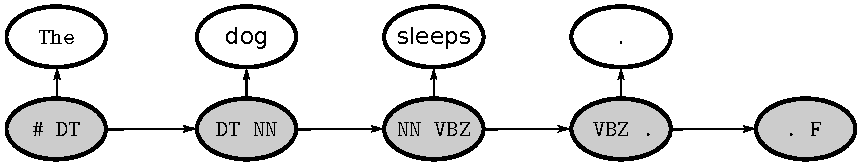
\includegraphics[scale=.7]{snd_order_path}
\caption{foo}\label{second-order-fig}
\end{center}
\end{figure}

The example with adverbs is poor at best, but it illustrates the kind
of effect {\it second order} information can have. Second order HMMs
are models where transitions are conditioned on two preceding hidden
states. Equivalently, in POS tagging, the hidden states can be taken
to be pairs of POS tags, e.g. {\tt DT, NN}. In such a model
transitions can only occur to a subset of the hidden state set. For
example a transition from {\tt DT, NN} to {\tt NN, VBZ} is possible,
but a transition to {\tt JJ, NN} is impossible. Figure
\ref{second-order-fig} illustrates a path with legal transitions. 

Figure \ref{second-order-fig} implies that emissions in a second order
model are conditioned on two labels like the transitions. However,
many existing HMM based POS tagging systems such as \cite{Brants2000}
condition emissions only on one label, that is use $e_{t_i, t_{i -
    1}}(w_i) = p(w_i \cond t_i)$ instead of $e_{t_i, t_{i - 1}}(w_i) =
p(w_i \cond t_{i - 1},\ t_{i})$. The reason is probably
data-sparsity. Therefore, these systems cannot be called HMMs in the
strictest sense of the word. They are instead called trigram
taggers. 

\cite{Halacsy2007}, show that it is possible to maintain the correct
HMM formulation over-come the data sparseness problem and achieve
gains over the more commonly used trigram tagger. However, they fail
to describe the smoothing scheme used, which is crucial. This defect
is partly remedied by the fact that the system is open-source.  One of
the chief contributions of \cite{Silfverberg2011} was to investigate
the effect of different ways of estimating the emission parameters in
a generative trigram tagger paying attention to smoothing.
 
Increasing model order unfortunately leads to increased data sparsity,
because the number of hidden states increases. Therefore, smoothing
transition probabilities is even more important than in the first
order case. Even using smoothing, third and higher order models tend
to generalize to unseen data more poorly than lower order models
because of over-fitting \citep{foo}.

An alternative to increasing model order, is to use so called latent
annotations \citep{Huang2009} in an otherwise regular first order
HMM. Conceptually, each label for example {\tt NN} is split into a
number of sub-states {\tt NN1}, {\tt NN2} and so on. Expectation
maximization is used to train the model in a partly supervised
fashion. Splitting labels, and indeed any increase in order, is
probably works better for label sets with quite few labels. Otherwise,
it will simply contribute data sparsity.

%\section{HMMs for POS Tagging}

\section{HMM taggers and Morphological Analyzers}
\label{sec:hmm-label-dict}
%\begin{itemize}
%\item Limiting transitions.
%\item How much of an improvement can be expected?
%\end{itemize}

The inventory of POS labels that are possible for a given word form
tends to be small. For example the English ``dog'' can get two of the
Penn Treebank POS tags singular noun {\tt NN} and {\tt VB} infinitive
verb form. The remaining 43 POS tags can never label
``dog''. Consequently, in an HMM POS tagger, only the states
corresponding to {\tt VB} and {\tt NN} should ever emit the word
``dog''.

A {\tt tag dictionary} \citep{Brants2000} can be used in combination
with the Viterbi algorithm to limit the set of hidden states that
could emit a word. The tag dictionary can be constructed from the
training corpus. Additionally, an external lexical resource, such as a
morphological analyzer, can be used. Such a lexical resource can help
to compensate for missing statistics for OOV words. In the frequent
setting, where most rare words have quite few analyses, this can have
a substantial effect on tagging accuracy.



\chapter{Generative Taggers using Finite-State Machines}
\label{chap:fsm}
In this Chapter, I will present an implementation of HMMs using {\it
  weighted finite-state machines}. It is further investigated in
Publications \ref{pub:1} and \ref{pub:2}. The implementation allows
for extensions of the HMM model in the spirit of \cite{Halacsy2007}
who utilize label context in the emission model of an HMM. It also
allows for applying global grammatical constraints. I will first
present a short summary of the most important aspects of finite-state
calculus and then present the finite-state implementation of HMMs.

\section{Weighted Finite-State Machines}

\paragraph{Automata} Weighted Finite-state automata are a data
structure for representing algorithms that solve the decision problem
of some regular language. A string can be either accepted or discarded
by a an automaton with some weight. Typically, weights bear
resemblance to probabilities and if they are interpreted as
probabilities, an automaton defines a distribution over the set of
strings. 

Figure \ref{fig:np-fsm} presents a finite-state which recognizes a
subset of noun phrases in the Penn Treebank. It illustrates the key
components of a finite-state automaton $M$
\begin{enumerate}
\item A finite set of states $Q_M$ ($\{0,\ 1,\ 2,\ 3,\ 4\}$ in Figure \ref{fig:np-fsm}).
\item An alphabet $\Sigma_M$ (the POS labels in Penn Treebank in Figure \ref{fig:np-fsm}).
\item A unique initial state $I_M$ ($0$ in Figure \ref{fig:np-fsm}).\footnote{Some formulations allow for several initial states with initial weights. This does, however, not increase the expressiveness of the formalism.}
\item A set of final states $F_M = \{r_1, ..., r_m\} \subset Q_M$ with associated final weights ${\rm f}(r_i)$ ($\{2\}$ and $1.0$ in Figure \ref{fig:np-fsm}).\footnote{Alternatively, we could also specify a final weight for every state. Then the actual final states would be the ones wit non-zero weight.}
\item A transition function $\tau_M$, which specifies a, possibly empty, set $\tau_M(q,x) = \{(q_1,w_1),\ ...,\ (q_n,w_n)\}$ of target states and transition weights for each symbol $x\in \Sigma_M$ in each state $q \in Q_M$ (in Figure \ref{fig:np-fsm} the relation is represented by the arrows in the graph).
\end{enumerate}
\begin{figure}[!ftb]
\begin{center}
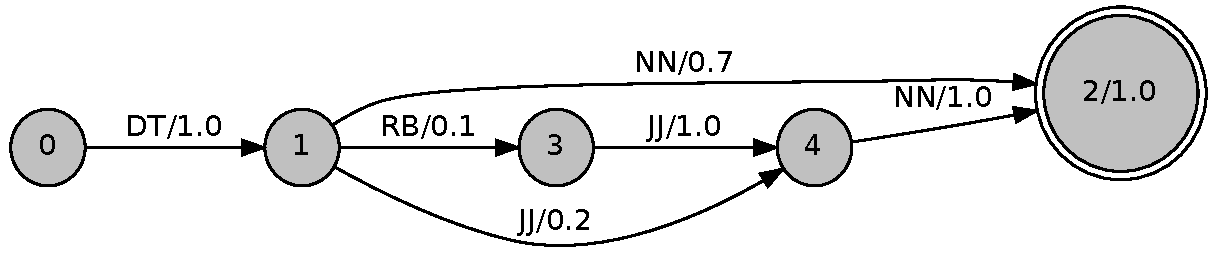
\includegraphics[scale=.7]{np}
\end{center}
\caption{A finite-state machine accepting a subset of the singular noun phrases in Penn Treebank.}\label{fig:np-fsm}
\end{figure}
When $\tau_M(a,q)$ is either empty or a singleton set for all $a$ and $q$, the automaton $M$ is called deterministic and I write $\tau_M(a,q) = (q_1,w_1)$ instead of $\tau_M(a,q) = \{(q_1,w_1)\}$.

\paragraph{Weight Semirings} Transition and final weights should form a
algebraical structure $\mathbb{K}$ called a semiring which is an abstraction of the
structure of positive real numbers under addition and multiplication. Consequently, two operations, addition $\oplus$ and
multiplication $\otimes$, are defined in $\mathbb{K}$. The addition operation should be
associative, commutative and have an identity element
$\mathbb{0}$. The multiplication operation should also be associative
and commutative. If it has an identity element, that element is
denoted by $\mathbb{1}$. The multiplication should distribute over the
addition \citep{Allauzen2007}.

As noted above, the prototypical example of a weight semiring is given by the positive real numbers together with the regular addition and multiplication of reals. This weight semiring, called the {\it probability semiring},\footnote{Even though the probability semiring is intended for representing probability distributions, weights cannot be restricted to $[0,1]$ the semiring has to be closed under addition.}  can be used to represent a probability distribution over the set of strings. In practice, this weight semiring is however rarely used. Because of numerical stability concerns, a logarithmic transformation $x \mapsto -log(x)$ is often applied to the weights and operations in the probability semiring. This gives the {\it log semiring}, where weights belong to $\mathbb{R}$, multiplication is given by $x \otimes y = x + y$ and addition by $x \oplus y = -\log(\exp(-x) + \exp(-y))$.

The addition operation of the log semiring $-\log(\exp(-x) + \exp(-y))$
is slow in practice. Moreover, $-\log(\exp(-x) + \exp(-y)) \approx y$
when $x \gg y$. Therefore, the addition operation in the log semiring
is often replaced by $x \oplus y = \min(x,y)$. This gives the {\it
  tropical semiring} which is the semiring used in this thesis.

I denote the transition weight of the transition leaving state $q_1$
with symbol $x$ and ending up in $q_2$ by $\w(\tau_M(q_1,x), q_2)$. As
a notational convenience, $\w(\tau_M(q_1,x), q_2) = \mathbb{0}$, if
there is no transition from $q_1$ to $q_2$. An automaton $M$ assigns a
weight to a path of states $p = (q_0,\ ...,\ q_{n+1})$, where $q_0 =
I_M$ and $q_n \in F_M$, and a string $s = s_1...s_n \in
\Sigma_M^{n}$. The weight is $\w_M(s,p)$ is given by Equation
\ref{eq:path-weight}. The total weight $\w_M(s)$ assigned to string
$s$ by automaton $M$ is given by Equation \ref{eq:string-weight}
\begin{equation}
\w_M(s,p) =
{\rm f}(q_{n+1})\otimes \bigotimes_{i = 0}^n \w_M(\tau_M(q_i,s_i), q_{i+1})\label{eq:path-weight}
\end{equation}

\begin{equation}
\w_M(s) =
\bigoplus_{p \in Q_M^{n+1}} \w_M(s,p) \label{eq:string-weight}
\end{equation}

\paragraph{Closure Properties} It is well known that regular languages
are closed under many unary and binary operations: union, negation,
concatenation and reversion \citep{Sipser1996}. Similarly, the class
of weighted finite-state machines is closed under these operations and
efficient algorithms for computing these operations exist. Table
\ref{tab:fs-algebra}, summarizes the properties of these algorithms.

\paragraph{N-Best}

\paragraph{Optimization} As stated above, a finite state machine where
each symbol and state is associated to maximally one transition is
called deterministic. It is well known that every finite-state machine
corresponds to a deterministic machine and this holds for weighted
finite-state machines as well \citep{Mohri2002}. A determinization
algorithm can be applied to any weighted finite-state machine in order
to produce a deterministic machine which accepts exactly the same set
of weighted strings as the original machine.

\begin{table}[!ftb]
\begin{center}
\begin{tabular}{lll}
Operation & Symbol & Definition \\
\hline
Power & $M^n$ & $\w_{M^n}(s) = \bigoplus_{s_1 ... s_n = s} \w_{M}(s_1) \otimes ... \otimes \w_{M}(s_n)$\\ 
Closure & $\bigoplus_{n = 0}^\infty M^n$ &  \\
Union & $M_1 \oplus M_2$ & $\w_{M_1 \oplus M_2}(s) = \w_{M_1}(s) \oplus \w_{M_2}(s)$\\ 
Concatenation & $M_1.M_2$ & $\w_{M_1.M_2}(s) = \bigoplus_{s_1s_2 = s} \w_{M_1}(s_1) \otimes \w_{M_2}(s_2)$\\
Intersection & $M_1 \cap M_2$ & $\w_{M_1 \cap M_2}(s) = \w_{M_1}(s) \otimes \w_{M_2}(s)$ \\
Composition & $M_1 \circ M_2$ & $\w_{M_1 \circ M_2}(s{\rm :}t) = \bigoplus_{r} \w_{M_1}(s{\rm :}r) \otimes \w_{M_2}(r{\rm :}t)$\\
\end{tabular}
\caption{A selection of operators for weighted finite-state machines
  given by
  \cite{Allauzen2007}.}\label{tab:fs-algebra}
\end{center}
\end{table}

%\paragraph{Transducers} Weighted finite-state automata solve the
%decision problem of regular languages with associated weights. In
%addition to this, a weighted finite-state transducer associates
%strings with a set of output strings. A WFST represent a {\it rational
%  relation} of strings. Whereas weighted automata can be seen as
%language models which weight each string, weighted transducers
%resemble analyzers or sequence labeling systems which output. Figure
%\ref{fig:np-fst} demonstrates this. It is a weighted analyzer for a
%few simple English noun phrases.

%The key difference between automata and transducers is the transition
%function. Unlike the transition function of an automaton, the
%transition function $\tau_M$ of a transducer $M$ maps a state $q$, an
%input symbol $x \in \Sigma_M$ and an output symbol $y \in T_M$ to a
%set of target states $\tau_M(q,x,y) \subset Q_M \times
%\mathbb{K}$. The sets $\Sigma_M$ and $T_M$ denote the input and output
%alphabet of the transducer $M$. Some transitions can lack an input or
%output symbol. A special empty string symbol $\epsilon$ is used to
%denote these. The input symbol of a transition therefore belongs to
%$\Sigma_M \cup \{\epsilon\}$ and the output symbol to $T_M \cup
%\{\epsilon\}$.

%The definition of the weight assigned by a transducer $M$ to paths and
%strings is very similar as in the case of automata. Given a path of
%states $p = (q_1,\ ...,\ q_{n+1})$, where $q_1 = I_M$ and $q_{n+1} \in
%F_M$, a sequence of pairs $u = ((s_1,t_1), ..., (s_n, t_n))$, where
%$x_i \in \Sigma_M \cup \{\epsilon\}$ and $y_i \in T_M \cup
%\{\epsilon\}$, the weight assigned to the path and pair sequence
%$\w_M(u,p)$ is given by Equation \ref{eq:fst-path-weight}. 

%Next, we will define the weight assigned to a string pair. Let $s \in
%\Sigma_M^*$ and $t \in T_M^*$, then a correspondence of $s$ and $t$ is
%a sequence of pairs $u = ((s_1,t_1), ..., (s_n, t_n))$, where $s_i \in
%\Sigma_M \cup \{\epsilon\}$, $t_i \in T_M \cup \{\epsilon\}$,
%$s_1...s_n$ equals $s$ except for some interleaved epsilons and the
%same holds for $t_1...t_n$ with respect to $t$. In this thesis I will
%assume that none of the pairs $(s_i,t_i)$ consists of two $\epsilon$
%symbols. This means that two strings $s$ and $t$ have only a finite
%number of correspondences. This simplifies the definition of the
%weight of a string pair. Let $c(s,t)$ be the finite set of
%correspondences of $s$ and $t$. Then the weight assigned to string
%pair $s{\rm : }t$ by transducer $M$, $\w_M(s{\rm :}t)$ is given by
%equation \ref{eq:fst-string-pair}.

%\begin{equation}
%\w_M(u,p) =
%{\rm f}(q_{n+1})\otimes \bigotimes_{i = 0}^n \w_M(\tau_M(q_i,x_i,y_i), q_{i+1}%)\label{eq:fst-path-weight}
%\end{equation}

%\begin{equation}
%\w_M(s{\rm :}t) =
%\bigoplus_{u \in c(s,t)} \bigoplus_{p \in Q_M^{|u| + 1}} \w_M(u,p) \label{eq:f%st-string-pair}
%\end{equation}

%\paragraph{Composition} Two transducers $M$ and $N$ represent weighted
%relations, $R_M$ and $R_N$ repsectively, between strings. It is
%possible to construct a weighted finite-state transducer which
%implements the relation $R_M \circ R_N$. The definition of this
%composition transducer $M \circ N$ is given in Table
%\ref{tab:fs-algebra}. Composition is a very useful operation because
%it allows for factorization of string transformations into simpler
%sub-transformation.

%Automata can be seen as a formalization of the concept of
%algorithm. They represent a restricted type of algorithm in the sense
%that they can only operate on symbol strings and they only operation
%they perform is to accept or reject a string. Although, this might
%sound quite restrictive, it turns out that most computational problems
%can be formalized as such {\it decision problems} involving only
%acceptance or rejection of symbol strings.

%Every automaton is associated with a {\it formal language} which is a
%(possible infinite) set of finite strings from the set of all strings
%of some finite alphabet. The automaton solves the decision problem of
%this language, i.e. accepts exactly those strings that belong to the
%language. {\it Weighted formal languages} are an extension to the
%concept of formal language, where each string should be assigned a
%weight. If the weights can be interpreted as probabilities, a weighted
%formal language over an alphabet $\Sigma$ can be seen as a probability
%distribution over the set of strings of the alphabet. However, this is
%not always possible because all weights cannot be interpreted as
%probabilities.

%Several well know classes of algorithms exist. The most famous ones
%are Turing machines which, in a sense, subsume all existing automata
%\cite{?}. In this thesis I have, however, utilized another class of
%automata, Finite-state machines. They are more restricted than Turing
%machines or another well know class, stack automata, because they
%utilize only a finite amount of memory. All real world implementations
%of automata of course utilize only a finite amount of memory.

%The restriction on memory limits the set of problems that finite-state
%machines can solve. However, at the same time it allows for a rich
%algebra which allows one to combine finite-state machines to produce
%new finite-state machines.

%The machine in Figure \ref{fig:np-fsm} accepts sequences of Penn
%Treebank labels which correspond to singular noun phrases that can
%have an adjective attribute (JJ) with an optional adverb (RB)
%expressing degree.

%Typically finite-state machines are represented as state transition
%graphs. An example is given in Figure \ref{fig:np-fsm}. The machine
%has a set of numbered {\it states} (0, 1, 2, 3 and 4) and {\it
%  transitions} from one state to another. The transitions are labeled
%using symbols from a finite alphabet (e.g. NN) and weights from a {\it
%  weight semiring}, when the machine is weighted. The weight semiring
%in this example is the {\it probability semiring} \cite{Allauzen2007}
%where weights are probabilities that can be added and multiplied in
%the usual fashion.

%Operation starts in the designated {\it start state} (0 in Figure
%\ref{fig:np-fsm}) and it has to end in a {\it final state} (2 in
%Figure \ref{fig:np-fsm} marked with a double ring). A string is
%accepted, if and only if there is a sequence of transitions leading
%from the start state to a final state where the symbols in the
%transition labels spell out the input string and the product of the
%weights along the path is non-zero. For example the machine in Figure
%\ref{np-fsm} accepts the string ``DT NN'' with weight 0.7 but rejects
%``DT JJ'' because the string inds when the machine is in state 4 but
%that is not a finite state.

%There may be several or no {\it accepting paths} for a given
%string. If there are several paths for some string, the machine is
%called {\it ambiguous}. More generally, a machine is called {\it
%  non-deterministic} if some state has several out-going transitions
%with the same label. Trivially, ambiguous machines are
%non-deterministic. In the case of ambiguous machines, the weight of a
%string is the sum of the weights of all of its accepting paths or zero
%if there are no accepting paths.


%\paragraph{Weighted formal languages} Formally, weighted languages are
%mappings $M : \Sigma^* \rightarrow \mathbb{K}$ from the set of
%arbitrary strings $\Sigma^*$ of some finite alphabet $\Sigma$ into
%some {\it weight semiring} $(\mathbb{K}, \oplus, \otimes, \mathbb{0},
%\mathbb{1})$ where $\mathbb{K}$ is a set of weights, $\oplus$ and
%$\otimes$ are addition and product operators for weights and
%$\mathbb{0} \in \mathbb{K}$ and $\mathbb{1} \in \mathbb{K}$ are the
%additive and multiplicative identity.

%\paragraph{Weight semirings} As mentioned above, the weight semiring
%in Figure \ref{fig:np-fsm} is the probability semiring, where weights
%belong to the set of non-negative reals $[0, \infty)$ and addition and
%product are given by the regular real addition and product
%operations. Even though probabilities reside in $[0,1]$, the addition
%of probabilities can result in quantities that are larger than
%$1$. Because finite-state algebra does include operations that add
%probabilities, the weight set needs to include all non-negative reals.

%The general weight semiring $(\mathbb{K}, \oplus, \otimes, \mathbb{0}, \mathbb{1})$ is an abstraction of the probability semiring. The set $\mathbb{K}$ is an arbitrary set but the operations $\oplus \rightarrow \mathbb{K} \times \mathbb{K} \rightarrow \mathbb{K}$ and $\oplus \rightarrow \mathbb{K} \times \mathbb{K} \rightarrow \mathbb{K}$ need to satify the following requirements \cite{Allauzen2007}
%\begin{enumerate}
%\item $(\mathbb{K}, \oplus, \mathbb{0})$ is a commutative and associative monoid.
%\item $(\mathbb{K}, \otimes, \mathbb{1})$ is an associative monoid.
%\item $\otimes$ distributes with respect to $\oplus$.
%\item $\mathbb{0}$ is the annihilator of $\otimes$.
%\end{enumerate}
%If $\oplus$ is a group operation, the semiring is in fact a ring. Many
%useful weight semirings are, however, not rings. Often the semiring
%$(\mathbb{K}, \oplus, \otimes, \mathbb{0}, \mathbb{1})$ is denoted
%simply as $\mathbb{K}$. Paralleling the regular sum notation $\Sigma_{i \in I} x_i$ and product notation $\prod_{i\in I} x_i$, I use the notations $\bigoplus_{i \in I} x_i$ and $\bigotimes_{i \in I} x_i$, where $I$ is a denumerable set.\footnote{Infinite sums and products are not defined in all semi rings, for example the probability semiring. In this case, it is often possible to augment the semirings with an infinity element $\infty$. This problem does not often cause problems in practice and will not be examined further.} Specifically $\oplus_{i \in \emptyset} x_i = \mathbb{0}$ and $\otimes_{i \in \emptyset} x_i = \mathbb{1}$.

%Weights in the probability semiring and the addition and product operations have an intuitive interpretation but from a practical point of view the probability semiring is sub optimal. The biggest drawback is that repeated multiplication of probabilities gives rise to very small quantities and under-flow becomes a problem. Therefore, the so called {\it logarithmic semiring} is more commonly used. It can be derived by applying a logarithmic transformation $x \mapsto -\log(x)$ to the weights and operations in the probability semiring. 

%In the logarithmic semiring, numerical under-flow is not a problem but
%the addition operation given by $x \oplus y = -\log(\exp(-x) +
%\exp(-y))$ is resource intensive. Therefore, another semiring, the
%{\it tropical semiring}, is often used. The addition operation in the
%tropical semiring is given by $x \oplus y = \min(x,
%y)$. Computationally, this operation is light. A theoretical
%motivation is given by the fact that $\min$ preserves the magnitude of
%the sum although not its exact value. In practice, this is often
%sufficient \cite{?}. All machines in this thesis use tropical
%weights.

%\paragraph{Weighted finite-state automata} Formally, a weighted
%finite-state automaton of weight semiring $\mathbb{K}$ is a structure
%$M = (\Sigma, Q, q_0, \rho, E)$ where
%\begin{enumerate}
%\item $\Sigma$ is a finite symbol set (also called an alphabet).
%\item $Q$ is a finite set of states.
%\item $q_0 \in Q$ is the unique start state.
%\item $\rho: Q \rightarrow \mathbb{K}$ is the final weight map.
%\item $T \subset Q \times (\Sigma \cup \{\epsilon\}) \times Q \times
%\mathbb{K} $ is a finite set of transitions.
%\end{enumerate}

%The final weight map $\rho$ associates each state $q \in Q$ with a final weight. The final states of $M$ are $\{q \in Q\ | \rho(q) \ne \mathbb{0}\}$.

%Each transition $x \in T$ consists of a source state $\s(x)$, an input symbol $\i(x)$, a target state $\t(x)$ and a weight $\w(x)$. The input symbol may be $\epsilon$ which denotes the empty symbol. For the single outgoing transition $x$ in state 4 in Figure \ref{fig:np-fsm}, the source state $\s(x) = 4$, the input symbol $\i(x) = {\rm "NN"}$, the target state $\t(x) = 2$ and the weight $\w(x) = 1.0$.

%A sequence of transitions $x_1, ..., x_n \in T$ is a {\it path}, if
% $\s(x_1) = q_0$ and $\t(x_{k-1}) = \s(x_k)$ for all $k$. As a special case, the empty
%sequence is also a path. The weight of path $p = (x_1, ..., x_n)$ is $\w_M(p) = ( \prod_{i = 1}^n \w(x_i) ) \otimes \rho(x_n)$ and the weight of the empty sequence is $\rho(q_0)$. A path $p$ is called successful when $\w_M(p) \ne \mathbb{0}$.

%Each path $p = (x_1, ..., x_n)$ is associated with a unique, possibly
%empty, string $s \in \Sigma^*$ such that there is a subsequence $j_i,
%..., j_m$ of $1, ..., n$ for which $i(x_{j_1}), ..., i(x_{j_m}) = s$
%and $i(x_{l}) = \epsilon$ whenever $l \notin \{j_1, ..., j_m\}$. If
%the path $p$ is associated with the string $s$, it is called a {\it
%  path of $s$}.

%The set of paths of a string $s$ is denoted $P_s$ and the weight
%assigned to $s$ by the automaton $M$ is $\w_M(s) = \bigoplus_{p \in
%  P_s} \w_M(p)$. When $P_s = \emptyset$, $\w_M(s) = \mathbb{0}$. The
%string $s$ belongs to the weighted language $L(M)$ accepted by $M$ if
%$L(M)(s) = \w_M(s) \ne \mathbb{0}$.

%\section{Finite-State Algebra}
%
%Finite-state machines use only a finite fixed amount of
%memory. Therefore, they cannot solve all computational problems. There
%is, for example, no finite-state machine which accepts only strings of
%prime number length. This can be proved using the pumping lemma of
%regular language \citep{Sipser1996} which are the languages whose
%decision problems finite-state automata can solve.
%
%Although the computational power of finite-state machines is limited,
%they are closed under a number of very useful operations which
%correspond to set theoretical operations of the languages recognized
%by the machines. The collection of these operations is called the {\it
%  finite-state algebra}.
%
%Table \ref{tab:fs-algebra} gives an overview of a number of well known
%finite-state operations.
%
%
%
%\section{Finite-State Transducers}
%Language processing frequently requires translation of one signal such
%as speech or text into another signal, for example text in another
%language in the case of machine translation or annotated text in the
%case of part of speech tagging. These do not seem like the kinds of
%processing tasks that finite-state machines can solve because, as we
%saw above, finite-state machines solve decision problems.
%
%Weighted Finite-state transducers are an extension of weighted
%finite-state automata. Whereas finite-state automata simply accept or
%reject a symbol sequence, finite-state transducers simultaneously
%output another symbol sequence.

%\begin{figure}
%\begin{center}
%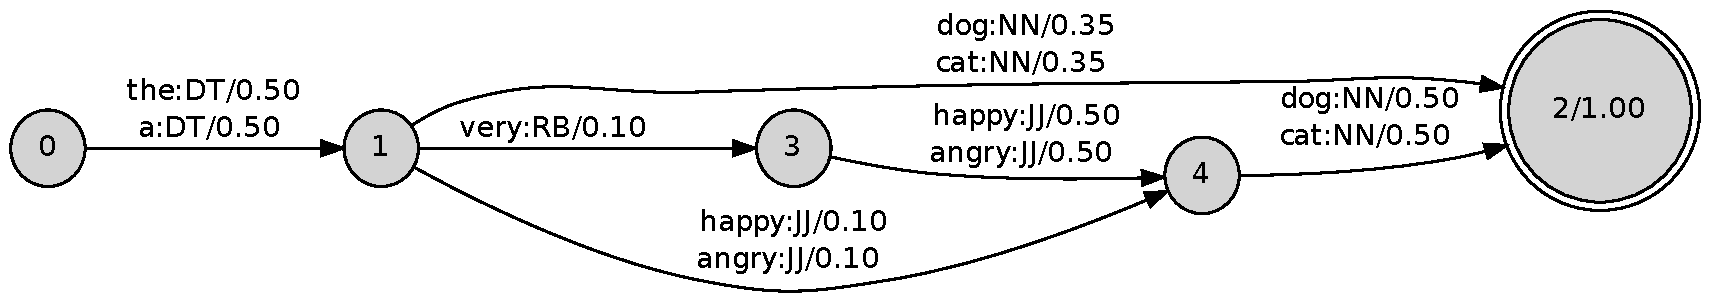
\includegraphics[scale=.5]{np_a}
%\end{center}
%\caption{A finite-state transducer that analyzes a subset of the singular noun% phrases in Penn Treebank.}\label{fig:np-fst}
%\end{figure}
%
%Formally, a weighted finite-state transducer of weight semiring
%$\mathbb{K}$ is a structure $M = (\Sigma, \Omega, Q, q_0, \rho, E)$ where
%\begin{enumerate}
%\item $\Sigma$ is a finite input symbol set (also called an input alphabet).
%\item $\Omega$ is a finite output symbol set (also called an output alphabet).
%\item $Q$ is a finite set of states.
%\item $q_0 \in Q$ is the unique start state.
%\item $\rho: Q \rightarrow \mathbb{K}$ is the final weight map.
%\item $T \subset Q \times (\Sigma \cup \{\epsilon\}) \times (\Omega \cup \{\epsilon\}) \times Q \times
%\mathbb{K} $ is a finite set of transitions.
%\end{enumerate}
%
%Transitions $e \in T$ are similar to transitions in automata but in
%addition to the input symbol $\i(e)$, they also contain an output
%symbol $\o(e)$. Paths of transitions are defined in the same way as
%paths for automata, however, paths of transducer transitions are
%associated with two strings -- an input and an output string. The
%input string of path $p = (x_1, ..., x_n)$ is the string $s_i =
%\i(x_1) ... \i(x_n)$ disregarding epsilons and the output string is
%$s_o = \o(x_1) ... \o(x_n)$ also disregarding epsilons. Path $p$
%itself is associated with the string pair $s = s_i \: s_o$. The set of
%paths associated with the input string of $s$ is $\P_i(s)$ and the set
%paths associated with of output string is $\P_o(s)$.
%
%The weight of path $p$ is defined in exaclty the same way as for
%automata 
%$$\w_M(p) = \Big( \prod_{i = 1}^n \w(x_i) \Big) \otimes \rho(x_n).$$
%
%A transducer $M$ can be viewed as a machine that maps input strings to
%sets of output strings with weights. Equivalently, it can be seen as a
%machine accepting string pairs $s = s_i \: s_o$ with some weight $\w_M(s)$. The
%weight $\w_M(s)$ given to string pair $s$ by transducer $M$ is defined 
%$$\w_M(s) = \bigoplus_{p \in \P_i(s) \cap \P_o(s)} \w_M(p)$$
%The defition takes into account the fact that there may be several
%alignments of input and output string giving the exact same string
%pairs. For example, $(\epsilon\:b, a\:b)$ and $(a\:b,\epsilon\:b)$
%represent the same string pair $a\:bb$.

\section{Finite-State Implementation of Hidden Markov Models} As seen
in Chapter \ref{chapter:hmm}, a generative HMM can be decomposed into
an emission model $p(x_i|y_i)$ of emissions $x_i$ given states $y_i$ a
transition model $p(y_{n+1} | y_1, ..., y_n)$, which models the
conditional distribution of a state $y_{n+1}$ given a state history
$y_1, ..., y_n$. As shown in Publications \ref{pub:1} and \ref{pub:2}
both of these can be compiled into weighted finite-state machines.

A generative HMM can be represented as a weighted finite-state machine
in several ways. The implementation presented in Publication
\ref{pub:1}, however, allows for enriching the emission model by
conditioning them on neighboring word forms and labels.

The main idea of the implementation discussed in Publication
\ref{pub:1} is to represent a labeled sentence as a string of word
form/label pairs as in Figure \ref{fig:lab-sent}. The emission and
transition models are implemented as weighted finite-state machines
which assign weights to such labeled sentences. Because of this
representation, both the emission model and transition model can
access information about the sequence of word forms and their
labels. Therefore, the emission and transition models can use more
information than in a regular HMM model. The sentence, emission and
different models are combined using the operations of finite-state
algebra.

In a normal HMM tagger, extension of the emission and transition model
requires changes to inference algorithms used by the tagger. In
contrast to a traditional HMM tagger, the finite-state tagger
presented in Publications \ref{pub:1} and \ref{pub:2} uses an n-best
paths algorithm for inference. This is a general algorithm which can
be applied on any model that can be represented as weighted
finite-state machine. Therefore, extending the emission and transition
models requires no changes to the inference procedure.

In this Section, I will discuss the implementation of a HMM model. In
the next Section, I will show how emission and transition models can
be extended.

\begin{figure}[!htb]
\begin{center}
\begin{tabular}{|l|l|l|l|l|l|l|l|}
\hline
The & DT & dog & NN & sleeps & VBZ & . & .\\
\hline
\end{tabular}
\caption{The representation of a labeled sentence as a single sequence.}\label{fig:lab-sent}
\end{center}
\end{figure}

\paragraph{Emission Model} Let $x = (x_1, ..., x_T)$ be a sentence and
let $Y_t = \{y_t^1, ..., y_t^n\}$ be the set of possible labels for
word $x_t$. Then we can construct a very simple finite-state machine
$X_t$ which recognizes the word $x_t$ and one of its possible labels
$y_t \in Y_t$ and assigns that combination a log weight corresponding
to the probability $p(x_t\cond y_t^i)$. As in the case of a regular HMM tagger,
$p(x_t\cond y_t)$ can be estimated from the training data. For OOV words,
we can use a guesser, for example the one presented in Chapter
\ref{chapter:hmm}.

As an optimization, only the most probable labels for each word can be
included in the emission model. However, it is completely possible to
include all labels for each word.

The individual emission machines $X_t$ can be combined into a sentence
model by concatenation as shown in Figure
\ref{fig:sentence-model}. The paths through the sentence model
correspond to the possible label assignments of sentence $x$.

\begin{figure}[!htb]
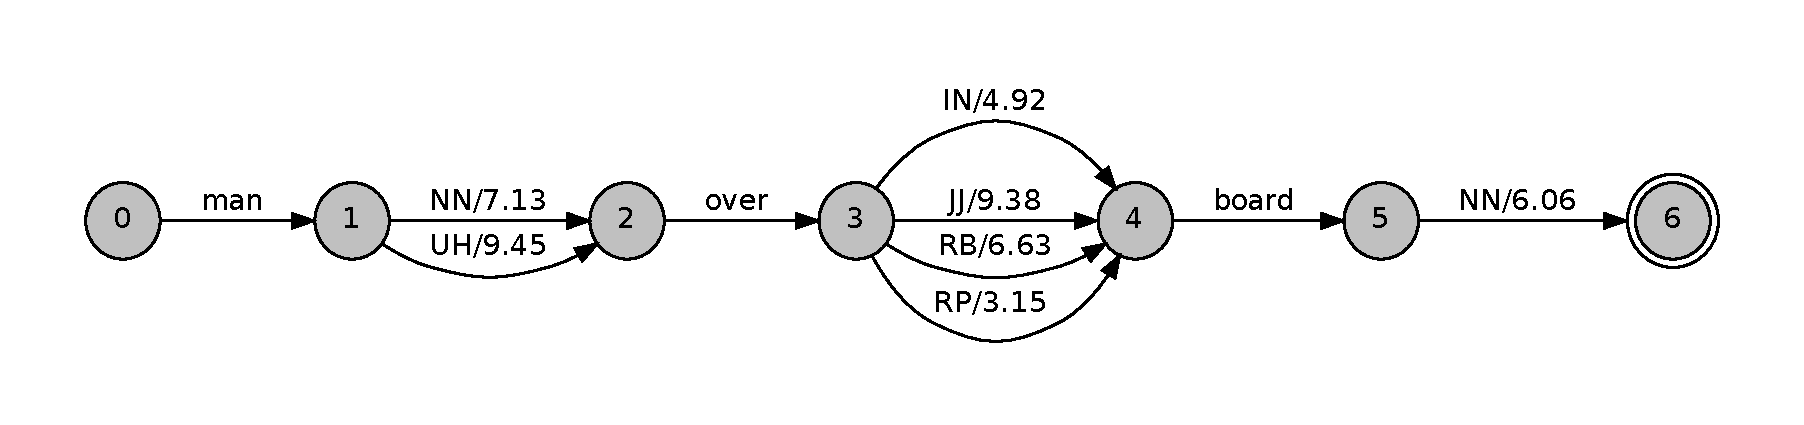
\includegraphics[scale=0.5]{sentence_model}
\caption{An example of a sentence model. The weights on the arcs are
  negative logarithms of emission probabilities. Only a subset of the
  possible labels are shown in the picture.}\label{fig:sentence-model}
\end{figure}

\paragraph{Transition Model} As stated above, Publications \ref{pub:1}
and \ref{pub:2} represent labeled sentences as a sequence of pairs
where each pair consists of a word form and a label. The transitions
model assigns weight to such sequences. I will explain the
construction of the transition model in three phases:
\begin{enumerate}
\item How to construct a model which assigns weight $-\log(p(y_{n+1}\cond
y_{1}, ..., y_{n}))$ to label n-gram $y_1, ..., y_{n+1}$.
\item How to extend the model to assign weight to an n-gram of word form/label pairs.
\item How to score an entire labeled sentence.
\end{enumerate}
The construction presented below will result in a number of
deterministic finite-state machines whose combined effect (the
intersection of the machines) corresponds to the n-gram model in a
standard HMM.

\paragraph{Scoring one label n-gram} The transition distributions $p(y_i\cond
y_{i - 1}, ..., y_{i - n})$ in an n-th HMM encodes the likelihood of
label sequences. I will first consider the problem of constructing a
machine which represents transitions weights for isolated label
n-grams. 

To emulate transitions weights in an HMM using finite-state calculus,
we can first compile a machine $T$ which accepts any sequence of $n+1$
labels $y_{1}, ..., y_{n+1}$. The weight assigned by the machine to
one of these paths can be estimated from a training corpus for the
sequences occurring in the corpus. Some form of smoothing is required
to score label n-grams missing from the training corpus. In
Publication \ref{pub:2}, a very simple form of smoothing is used. Each
n-gram not occurring in the training corpus will receive an identical
penalty weight $-\log(1/(N+1))$, where $N$ is the size of the training
corpus. Additionally, Publication \ref{pub:2} uses interpolation of
probability estimates of n-grams of different orders. More
sophisticated smoothing schemes could also be applied at the cost of
larger model sizes.

[WRITE ABOUT DETERMINIZATION AND MINIMIZATION]

If the machine $T$ is deterministic and has one path corresponding to
each label n-gram $y_1, ..., y_{n+1}$, where $y \in \mathcal{Y}$, each
non-terminal state in the machine will have $\mathcal{Y}$
transitions. Because $T$ encodes the weight $p(y_{n+1}\cond y_{1},
..., y_{n})$ for each label n-gram, it will have a large amount of
states when many label n-grams occur in the training corpus. It is
difficult to present a formal analysis of the size of $T$ as a
function of the number of distinct label n-grams in the corpus. An
example can, however, illustrate the number of states that are
typically required.

For the FinnTreeBank corpus, 8801 non-terminal states are required to
represent $T$ for $n=2$. As the corpus has $1399$ distinct
morphological labels, this translates to approximately 12 million
transitions. When using add one smoothing, most label n-grams will
have the same weight.

If the machine $T$ is deterministic and has one path
corresponding to each label n-gram $y_1, ..., y_{n+1}$, where $y \in
\mathcal{Y}$, each non-terminal state in the machine will have
$\mathcal{Y}$ transitions. Because $T$ encodes the weight
$p(y_{n+1}\cond y_{1}, ..., y_{n})$ for each label n-gram, it will
have a large amount of states when many label n-grams occur in the
training corpus. It is difficult to present a formal analysis of the
size of $T$ as a function of the number of distinct label n-grams in
the corpus. An example can, however, illustrate the number of states
that are typically required.

For the FinnTreeBank corpus, 8801 non-terminal states are required to
represent $T$ for $n=2$. As the corpus has $1399$ distinct
morphological labels, this translates to approximately 12 million
transitions. When using add one smoothing, most label n-grams will
have the same weight.

In order to, reduce the size of the model, so called {\it failure
  transitions} can be used \citep{someone}. A failure transition in a
state $q$, will match any symbol which does not have another outgoing
transition in $q$. The failure transitions will go to sink states,
which encode the penalty weight for unseen label n-grams.  Using
failure transitions, most states will not have $|\mathcal{Y}|$
transitions. Because of data sparsity, most state will in fact have
only a few outgoing transitions. Figure \ref{fig:fail_t} illustrates a
bigram model with failure transitions.

\begin{figure}
\begin{center}
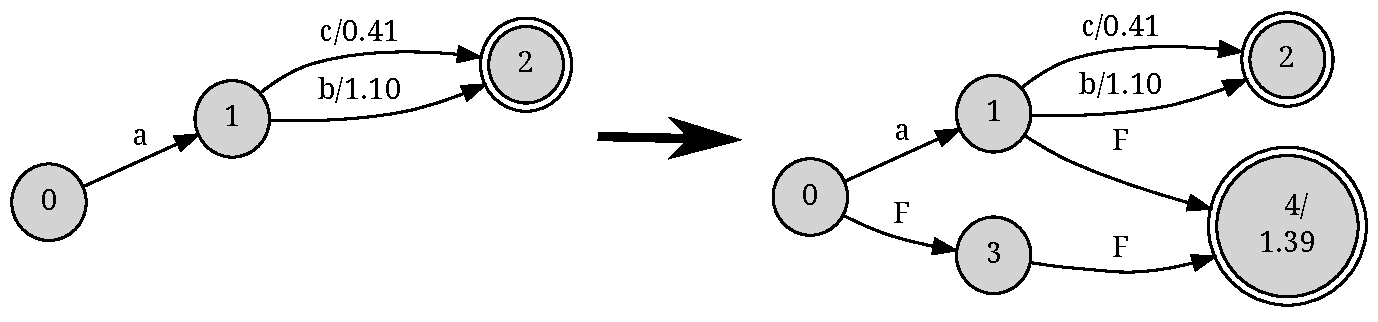
\includegraphics[scale=0.5]{fail_t}
\caption{Failure transitions (with symbol F) are added to a bigram model.}\label{fig:fail_t}
\end{center}
\end{figure}

I will now outline the procedure to compute a machine with failure
transitions in the general case. We first need an auxiliary
definition. For a state $q \in Q_T$, let $n(q)$ be the length of the
shortest symbol string required to reach state $q$ from the initial
state $q_0$.  Now, given a machine $T$ that recognizes every label
n-gram occurring in the training corpus, a corresponding machine $T_f$
with failure transitions can be computed.

\begin{enumerate}
\item $n+1$ new sink states are added: $Q_{T_f} = Q_T \cup \{s_1, ...,
  s_{n+1}\}$. The state $s_{n+1}$ is final and its final weight is the
  penalty weight for unseen n-grams.
\item A failure symbol is added: $\Sigma_{T_f} = \Sigma_T \cup \{f\}$, where $f \notin \Sigma_T$.
\item $\tau_{T_f}(q,a) = \tau_T(q,a)$ for all $q \in Q_T$ and $a \in \Sigma_T$. 
\item $\tau_{T_f}(s_1,f) = \{(s_{i+1}, \mathbb{1}\}$ for $i <= n$.
\item Failure transitions are added: $\tau_{T_f}(q, f) = \{(s_{n(q)}, \mathbb{1})\}$.
\end{enumerate}

\paragraph{Adding word forms} The current transition model scores
label n-grams. However, because we represent labeled sentences as
sequences of word form/label-pairs, we need to include word forms in
the model. This can be accomplished by adding a number of new states
and failure transitions to the model. When implementing a standard HMM
tagger, the added failure transitions will simply skip word
forms. Figure \ref{fig:fail_t_wf} demonstrates the construction for
the transition model in Figure \ref{fig:fail_t}.

\begin{figure}[!htb]
\begin{center}
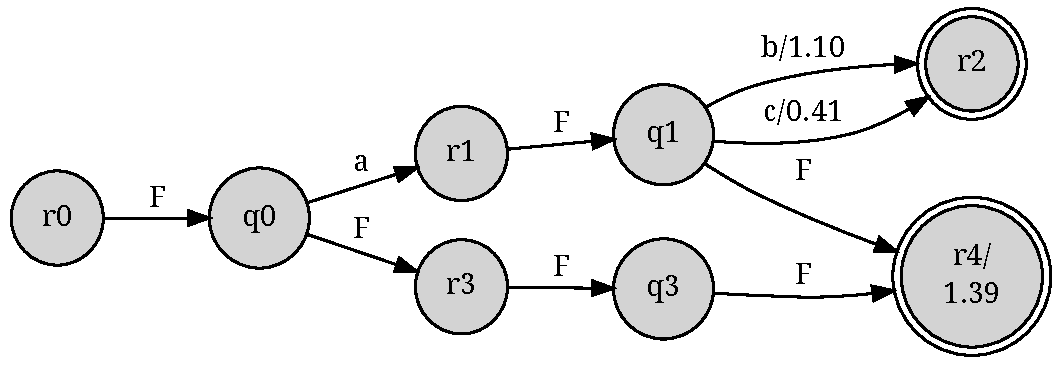
\includegraphics[scale=0.5]{fail_t_wf}
\caption{The transition model in Figure \ref{fig:fail_t} is augmented
  with failure transitions and states in order to be able to handle
  word forms.}\label{fig:fail_t_wf}
\end{center}
\end{figure}

We construct a new machine $T_w$ which accepts n-grams of word
form/label-pairs. Let $Q_{T_f} = \{q_0, ..., q_k\}$, then $Q_{T_w} =
Q_{T_f} \cup {r_0, ..., r_k}$, where $r_i \notin Q_{T_f}$. Let $r_0$
be the start state of $Q_{T_f}$ and let $F_{T_f} = F_{T_w}$. The
transitions function $\tau_{T_w}$ is defined in the following way.

\begin{enumerate}
\item $\tau_{T_w}(r_i,f) = \{(q_i,\mathbb{1})\}$.
\item $\tau_{T_w}(q_i,x) = \{(r_j,w)\}$ for all $x \in \Sigma_{T_w}$, if $\tau_{T_f}(q_i,x) = \{(q_j,w)\}$.
\end{enumerate}

Consider two states $q_1,q_2 \in Q_M$, in a machine $M$ with failure
transitions. Failure transitions in $q_1$ and $q_2$ may match a
different set of symbols. For example, If $q_1$ has a transition with
symbol $a \in \Sigma_M$ and $q_2$ does not, then $a$ will match the
failure transition in $q_2$ but it will not match the failure
transition in $q_1$. This is a problem when the determinization
algorithm is applied to $M$ because determinization joins states.
State joining may change the language accepted by $M$ and the
weights assigned to strings. 

It is highly desirable that the transition model of the finite-state
implementation of an HMM tagger is deterministic because of reduced
tagging time. However, as noted above, we cannot use standard
determinization with machines which have failure
transitions. Therefore, the construction presented below will produce
deterministic machines without resorting to determinization.

\paragraph{Scoring a sentence} We will now see how the transition
model for scoring an isolated label n-gram can be extended for scoring
an entire sentence. Given the machine $T_w$ which scores one n-gram,
we can form the Kleene closure of $T_w$. Since $M_n$ is an acyclic
machine accepting strings of equal length (that is $2n$: $n$ word
forms and $n$ labels), we can easily compute a deterministic Kleene
closure $T_{w}^*$ of $T_w$ by re-directing transitions going to final
states into the initial state\footnote{It can easily be seen that this
  construction fails if the machine accepts strings of unequal
  lengths.}
\begin{enumerate}
\item $\Sigma_{T_w^*} = \Sigma_{T_s}$. 
\item $Q_{T_w^*} = Q_{T_w} - F_{T_w}$.
\item $F_{T_w^*} = \{q_0\}$ and $f(q_0) = \mathbb{0}$.
\item $\tau_{T_w^*}(a,q) = \{(q', w)\}$, if $\tau_{T_w}(a,q) = \{(q',
  w)\}$ and $q'\notin F_{T_w}$.
\item If $\tau_{T_w}(a,q) = \{(q', w)\}$ and $q' \in F_{T_w}$, then
  $\tau_{T_w^*}(a,q) = \{(q_0, w + f(q'))\}$.
\end{enumerate}

The machine $T_{w}^*$ will score entire labeled sentences, however, it
only scores some of the trigrams in the sentence, namely, the ones
starting at positions divisible by $n+1$. Fortunately we can form $n +
1$ machines $T_0$ ... $T_n$ which will score all remaining
n-grams. Let $T_0 = T_{w}^*$ and let $T_{i+1} = F.F.T_i$. Intuitively
each $T_i$ will skip $i$ word form/label-pairs.

The final scoring of all possible labeled sentences, corresponding to
an input sentence $x$, is accomplished by intersecting the sentence
model $X$ and each of the $T_i$ using an intersection algorithm which
handles failure symbols correctly. In Publications \ref{pub:1} and
\ref{pub:2} a parallel intersection algorithm \citep{Silfverberg2009},
however, this is not actually required. The intersections can be
performed sequentially.

\paragraph{Smoothing} As observed in Chapter \ref{chapter:hmm}, a
second order model usually gives the best results in morphological
tagging. However, a pure second order model suffers from data sparsity
which degrades it performance. This can be avoided using smoothing. In
Publications \ref{pub:1} and \ref{pub:2}, smoothing is accomplished by
using first and zeroth order transition models in addition to the
second order transition model. To get the combined effect of all
models, each of them is intersected with the sentence model.

Usually, for example in \cite{Brants2000}, the transition
probabilities $p(y_i|y_{i-1}, y_{i-2})$ are a linear interpolation of
the probability estimates $\hat{p}$ for different orders as shown in
equation \ref{eq:ip}. \cite{Brants2000} sets the values for $\alpha_i$
using deleted interpolation and cross validation. When $\sum_i
\alpha_i = 1$, it is easily seen that Equation \ref{eq:ip} defines a
probability distribution over $y_i$.

\begin{equation}
p(y_i|y_{i-1}, y_{i-2}) = \alpha_2\hat{p}(y_i|y_{i-1},y_{i-2}) + \alpha_1\hat{p}(y_i|y_{i-1}) + \alpha_0\hat{p}(y_i)\label{eq:ip}
\end{equation}

Linear interpolation is not possible when using the finite-state
implementation presented in this chapter because intersection of
weighted machines corresponds to multiplying probability estimates,
not to adding them. Therefore, Publications \ref{pub:1} and
\ref{pub:2} define the score $s(y_i|y_{i-1}, y_{i-2})$ of a labeled
sentence as the weighted product given in Equation
\ref{eq:ip-fsm}. Inference corresponds to finding the label sequence
which maximizes the score. The optimal values for the exponents
$\alpha_i$ in Equation \ref{eq:ip-fsm} are found by optimizing the
tagging accuracy on held out data using grid search.

\begin{equation}
s(y_i|y_{i-1}, y_{i-2}) = \hat{p}(y_i|y_{i-1},y_{i-2})^{\alpha_2} \hat{p}(y_i|y_{i-1})^{\alpha_1}\hat{p}(y_i)^{\alpha_0}\label{eq:ip-fsm}
\end{equation}

The weighted product $s(y_i|y_{i-1}, y_{i-2})$ given by
\ref{eq:ip-fsm} does not necessarily define a probability distribution
over $y_i$. It can, however, easily be normalized to give one. When the
score is normalized, it can be seen as a special case of the family of
distributions defined by Equation \ref{eq:ip-general}. Here the
parameter values $r_2(y_i|y_{i-1},y_{i-2})$, $r_1(y_i|y_{i-1})$,
$r_0(y_i)$ can be arbitrary positive real numbers. Each assignment of
the parameter values defines a probability distribution over $y_i$.

\begin{equation}
p(y_i|y_{i-1}, y_{i-2}) = \frac{r_2(y_i|y_{i-1},y_{i-2})r_1(y_i|y_{i-1})r_0(y_i)}{\sum_{y\in\mathcal{Y}} r_2(y|y_{i-1},y_{i-2})r_1(y|y_{i-1})sr0(y)}\label{eq:ip-general}
\end{equation}

The interpretation of the weighted product in Equation \ref{eq:ip-fsm}
given by Equation \ref{eq:ip-general} reveals a problem. There is no
guarantee that the parameter values $r(y_i|y_{i-1},y_{i-2}) =
\hat{p}(y_i|y_{i-1},y_{i-2})^{\alpha_2}$, $r_1(y_i|y_{i-1}) =
\hat{p}(y_i|y_{i-1})$ and $r_0(y_i) = \hat{p}(y_i)^{\alpha_0}$ result
in a model which fits the training data maximally well in the sense
that is discussed in Chapter \ref{chap:ml}. This may have contributed
to the inferior tagging accuracy of the system when compared to
\cite{Brants2000} which is seen in the experiments in Publication
\ref{pub:2}. This problem lead the
author to consider conditional random fields presented in Chapter
\ref{chapter:crf}, which naturally support a product formulation.

\section{Beyond the Standard HMM}\label{sec:enriched}

The real strength of the system presented in this chapter lies in its
capability of easily incorporating information not usually present in
a generative HMM tagger. \cite{Halacsy2007} show that enriching the
emission model of an HMM tagger by including label context can improve
tagging results. Instead of the usual emission model $p(x_t\cond y_t)$
which conditions each word on its morphological label,
\cite{Halacsy2007} instead use a model $p(x_t\cond y_{t-1},y_t)$,
where the emission is conditioned on preceding label context. As
stated in Chapter \ref{chapter:hmm}, this is in fact not an extension
to the standard second order HMM. Instead, it is the faithful
implementation of the second order HMM model. The usual definition
$p(x_t\cond y_t)$ is incorrect in a second order HMM. It is probably
used because of data sparsity. Nevertheless, \cite{Halacsy2007} show
that the correct formulation can result in improved tagging accuracy.

\paragraph{Richer local structure} The model presented by
\cite{Halascy2007} can easily be implemented as a finite-state machine
by a slight modification to the compilation of the sentence model as
described in Publication \ref{pub:1} and it can be extended to model
$p(x_t\cond y_{t-1}, y_t, y_{y+1})$. Moreover, it is possible to
condition transitions on word forms as shown in Publication
\ref{pub:1}. Both of these modifications are shown to give
statistically significant improvements over the standard baseline
model. The problem with including such information in the emission and
transition models is that it violates the conditional independence
assumptions in the generative HMM model. This is yet another reason to
consider alternative models such as the conditional random field or
averaged perceptron.

\paragraph{Global Constraints} In addition to local changes to the
emission and transition models, it would also be possible to include
global probabilistic constraints to the model. These are constraints
that apply on the entire input sentence. A simple example of such a
constraint is the existence or frequency of finite verb forms in the
sentence. Another family of interesting global constraints is given by
syntactic and semantic valency of words \citep{Baker1998}. Such
information could be represented as a weighted finite-state
machine. Similarly to the enriched locally emission and transition
models, global constraints also violate the independence assumption of
the generative HMM model.

%\chapter{Generative Taggers using Finite-State Transducers}

%This section presents a finite-state implementation of generative
%taggers such as HMMs using finite-state algebra. This expands on
%Publications \ref{pub:1} and \ref{pub:2}.

%\begin{itemize}
%\item \cite{Halacsy2007} and Publication \ref{pub:2}.
%\end{itemize}


%\paragraph{Emission model}
%\paragraph{Transitions Model}
%\paragraph{Global constraints}

%\section{Problems} In the standard first order HMM an observation
%depends only on the current hidden state. If the hidden state is
%given, the observation cannot be influenced by the hidden states at
%other positions in the input or the other observations. This
%facilitates estimation and makes the system resistant to over-fitting,
%but at the same time it severely limits the set phenomena that the model
%can capture.

%An example from POS tagging the Penn Treebank illustrates this
%problem. The Penn Treebank has two labels for common nouns: {\tt NN}
%for singular nouns and {\tt NNS} for plural nouns.

%\begin{itemize}
%\item Local normalization.
%\item Inability to use word context.
%\item Label bias.
%\item The inability to use rich features, causes problems in domains
%other than POS tagging and in POS tagging for MR languages.
%\item Smoothing is difficult.
%\item Differences in performance between generative HMMs and
%discriminative approaches are even greater for morphologically complex
%languages and small training sets.
%\item OOV words may require different mechanisms depending on language
%again causing problems for MR lanuages.
%\end{itemize}

\section{Summary of Publications \ref{pub:1}, \ref{pub:2} and \ref{pub:3}}

Publication \ref{pub:1} presents the finite-state implementation of
HMMs introduced in this Chapter and Publication \ref{pub:2} presents
experiments using the model on the Penn Treebank and a Finnish data
set. The taggers presented in Publications \ref{pub:2} are used in
Publication \ref{pub:3} to implement a language model for a
context-sensitive finite-state spelling corrector.

\paragraph{Publication \ref{pub:1}} The main contribution of this
publication is to present the finite-state implementation of HMMs. The
publication presents experiments on morphological tagging of Finnish,
English and Swedish but the experiments presented in the publication
are nearly void of value because they were conducted on machine
labeled data and the amount of training data was unrealistic (1
million sentences for each language). Both factors contribute to
extremely good, and quite unrealistic, tagging accuracy for all
languages on test data. Still, the extreme size of the training set
does demonstrate that the method can use large amounts of training
data.

For Finnish, experiments on machine labeled data were the only option
because, at the time, there was no freely available hand-labeled
morphologically tagged corpus available. For Swedish and English,
established data sets should have been used.

The formulation of the probabilistic model in Publication \ref{pub:1}
differs from the formulation in this Chapter in two respects. Instead
of the usual transitions probabilities $p(y_{t}\cond y_{t-n}, ...,
y_{t-1})$, Publication \ref{pub:1} uses the joint probability
$p(y_{t-n}, ..., y_t)$. The model can therefore not be seen as an
actual HMM. Additionally, the publication uses lexicalized transition
probabilities. The final probability is thus $p(l_{t-n}, y_{t-n}, ...,
l_t, y_t)$, where the $l$ refer to lemmas. This is possible because of
the extremely large training set.

Although the experiments in Publication \ref{pub:1} are flawed, the
paper is included in the thesis because it describes the finite-state
implementation for HMM taggers and can be seen as a natural starting
point for Publications \ref{pub:2} and \ref{pub:3}.

\paragraph{Publication \ref{pub:2}} The main contribution of this
publication is to present experiments on a standard data set for POS
tagging of English, the Penn Treebank 2. However, because of
insufficient knowledge at the time, the experiments were performed on
a non-standard version of Penn Treebank 2. Publication \ref{pub:1}
uses the data splits introduced by \cite{Collins2002} but the data
from the {\tt tagged} sub-directory in the Penn Treebank 2
distribution. As \cite{Toutanova2003} explain, it is conventional to
extract the POS tagged sentences from the parse trees in the {\tt
  parsed} sub-directory in the distribution. Unfortunately, this makes
the reported accuracies approximately 0.3 \%-points higher than they
would be if the experiments were performed on the correct data
set. For Finnish, experiments were performed on machine labeled data by
necessity, similarly as in the case of Publication \ref{pub:1}.

Publication \ref{pub:2} presents models for Finnish and English which
use enriched emission models described in Section \ref{sec:enriched},
which are inspired by the HunPos system \citep{Halacsy2007}. The
taggers are evaluated against a standard HMM baseline. The results are
also compared against tagging accuracies reported in \cite{Brants2000}
and \cite{Halacsy2007}. Because of the unfortunate mix-up with the
Penn Treebank data set, the results for English are not comparable
between the different tagging systems. However, Publication
\ref{pub:2} does show that the enriched emission models yield clear
improvements over baseline. Moreover, the final system outperforms
HunPos by 0.4\%-points on the Finnish data set. Because the data set
is machine labeled, this result may of course not be convincing.

\paragraph{Publication \ref{pub:3}} This publication applies the
taggers presented in Publications \ref{pub:1} and \ref{pub:2} to the
task of context-sensitive spelling correction. Many spelling
correction systems determine the best spelling correction for a
misspelled word based solely on the misspelled word form
itself. Typically, correction candidates that have a small edit
distance to the misspelled word form are ranked higher than more
remote candidates. Context-sensitive spelling correction systems
additionally utilize surrounding words to rank correction candidates.

For English, plain word context can improve the accuracy of spelling
correction \citep{Brill2000}. For example ``cat'' is much more likely
in the context ``the _ miaowed'' than ``car'' is. As Publication
\ref{pub:2} shows, word context does improve results for Finnish as
well. However, Publication \ref{pub:3} also shows that a morphological
tagger can yield greater improvements in accuracy for both English and
Finnish when using comparable amounts of training data for the tagger
and word context model. Of course, the word context model can be
trained on unlabeled data. Therefore, there is in principle no
obstacle to using arbitrarily much training data.

The system presented in Publication \ref{pub:3} first generates a set
of correction candidates for the misspelled word using a finite-state
spelling correction system based on edit distance. It then uses a
generative morphological tagger for selecting the best candidate. The
misspelled form is replaced with each correction candidate $c_1$, ...,
$c_n$ in turn producing $n$ sentences $x_1$, ..., $x_n$. The sentences
are then tagged which results in $n$ tag sequences $y_1$, ...,
$y_n$. The candidates $c_i$ are finally ranked according to the joint
probability of the sentence and label sequence
$p(y_i,x_i)$.\footnote{In fact only a sub-sequence of the sentence is
  tagged as an optimization, however, the basic idea is the same.}

The spelling correction system using the morphological tagger probably
yields better results, especially for English, because it is less
susceptible to data sparsity than the word context model. As noted
above, the amount of training data for the word context model could,
however, be increased. This is likely to gradually improve
accuracy. At the same time it, however, increases the size of the
model. The spelling correction system that uses the morphological
tagger can be more compact and thus more practicable while delivering
comparable accuracy.


%\chapter{Generative Taggers using Finite-State Transducers}

This section presents a finite-state implementation of granarative taggers such as HMMs using finite-state algebra. This exapnds on Publications \ref{pub:1} and \ref{pub:2}.

\section{Enriching the emission and transition models}
\begin{itemize}
\item \cite{Halacsy2007} and Publication \ref{pub:2}.
\end{itemize}

\section{Problems}
In the standard first order HMM an observation depends only on the
current hidden state. If the hidden state is given, the observation
cannot be influenced by the hidden states at other positions in the
input or the other observations. This facilitates estimation and makes
the system resistant to over-fitting, but at the same time it severly
limits the set phenomena tht the model can capture.

An example from POS tagging the Penn Treebank illustrates this
problem. The Penn Treebank has two labels for common nouns: {\tt NN}
for singular nouns and {\tt NNS} for plural nouns.

\begin{itemize}
\item Local normalization.
\item Inability to use word context.
\item Label bias.
\item The inability to use rich features, causes problems in domains
  other than POS tagging and in POS tagging for MR languages.
\item Smoothing is difficult.
\item Differences in performance between generative HMMs and
  discriminative approaches are even greater for morphologically
  complex languages and small training sets.
\item OOV words may require different mechanisms depending on
  language again causing problems for MR lanuages.
\end{itemize}


\section{Finite-State Implementation of Hidden Markov Models}
As seen in Chapter~\cite{chapter:hmm}, an HMM can be decomposed into a
emission model, which models the conditional distribution $p(y|x)$ of
all labels $y$ given a state $x$ and a transition model, which models
the conditional distribution $p(y_{n+1} | y_1, ..., y_n)$ of states
$y_{n+1}$ given a state history $y_1, ..., y_n$.

Both the emission and transition models can be compiled into
finite-state machines. The emission model is compiled into one
finite-state transducer but the transition model is made up from a
number of component models. All the models are combined using a
run-time variant of composition and intersection.

\paragraph{Interpreting HMMs as Finite-State Machines}
Given a sequence of observations $x = (x_1, ..., x_n)$ and states $y = (y_1, ..., y_n)$, the joined probability for $x$ and $y$ given by an HMM with parameters $\theta$ is 
$$p(x,y\parcond\theta) = p(y\parcond\theta)\cdot p(x \cond y\parcond\theta)= \Bigg(\iota(y_1) \cdot \prod_{t = 1}^{T} \tau_{y_t}(y_{t + 1})\Bigg) \cdot \prod_{t = 1}^T \varepsilon_{y_t}(x_t)$$
where $\iota$, $\tau$ and $\epsilon$ are initial, transition and emission distributions respectively.

In an HMM the states $y_i$ correspond to actual states of the
model. When interpreting an HMM as a finite-state transducer, they
will instead correspond to output symbols. The transducer will then
map the input sequence $x$ to the states sequence $y$ with weight
$p(x,y\parcond\theta)$.

\cite{Mohri2002} describe an implementation of HMMs for speech
recognition where each individual phoneme can be recognized by a small
HMM. Their construction, however, requires $O(|Y|)^n$ states where $Y$
is the set of states of the HMM and $n$ its order. It is easy to see
that this is infeasible. For example when using a second order model
with a morphological label set of 1000 labels the resulting transducer
has around one billion states.

\paragraph{The Emission Model}
foo

\paragraph{The Transition Model}
bar

\paragraph{Weighted Intersecting Composition}
baz

\chapter{Conditional Random Fields}

\section{Discriminative modeling}

As seen in Chapter \ref{chapter:hmm}, the HMM POS tagger can be viewed
as a state machine which alternates between sampling words from state
specific observation distributions and sampling morphological labels
from state specific transition distributions. Each emission word and each
morphological label is conditioned {\it solely} on the current
morphological label. These independence assumptions are harsh. For example
collocations cannot be adequately modeled, because the model does not
include direct information about neighboring words in a sentence.

Although information about word sequences and orthography is quite
useful in morphological labeling, it is often difficult to incorporate
such information in a generative model. As \cite{Sutton2012} note, two
principal approaches could, however, be attempted:
\begin{enumerate}
\item Extending the emission model presented in Chapter
  \ref{chapter:hmm} to incorporate dependencies between words and
  orthographic features.\label{ap:1}
\item Replacing the usual emission model with a Naive
  Bayes' model which in theory can handle arbitrary
  features (although overlapping features cause ).\label{ap:2}
\end{enumerate}

Approach \ref{ap:1} is difficult in a fully generative setting because the
emission model needs to account for the complex dependencies that
exist between sentence contexts and orthography. There simply does not
seem to exist a straightforward way of modeling the dependencies.

In a domain closely related to morphological labeling, namely
biomedical entity extraction,\cite{Ruokolainen2013} show that approach
\ref{ap:2} also fails. In fact their experiments indicate that adding richer
context modeling such as adjacent words may worsen the performance of
a tagger with a Naive Bayes emission model. One reason for this may be
that overlapping information sources required in a rich emission model
tend to cause the Naive Bayes model to give overly confident
probability estimates \citep{Sutton2012}. Combining the probabilities
given by the emission model with the transition model can therefore be
problematic.

In contrast to generative sequence models, discriminative sequence
models such as Maximum Entropy Markov Models \citep{Ratnaparkhi1998}
and Conditional Random Fields \citep{Lafferty2001} can incorporate
overlapping sources of information. They model the conditional
distribution of label sequences $p(y\cond x)$ directly instead of
modeling the joint distribution $p(x,\ y)$. Therefore, they do not
need to model the distribution of sentences at all. 

Discriminative models assign probabilities $p(y\cond x)$ for label
sequences $y = ({\rm DT},\ {\rm NN},\ {\rm VBZ},\ {\rm .})$ and word sequences $x = ({\rm The},\ {\rm dog},\ {\rm eats},\ {\rm .})$ by extracting local features from
the input sentence and label sequence. Examples of local features
include {\it ($x_1$ is ``dog'' and $y_1$ is ``NN'')} and {\it ($y_{0}$ is ``DT'' and
  $y_1$ is ``NN'')}. Each feature is associated with a parameter value and the
parameter values are combined to give the conditional likelihood of
the entire label sequence. Naturally, the label sequence which
maximizes the conditional likelihood given sentence $x$ is the label
sequence returned by the discriminative POS tagger.

In generative models, emissions and transitions are independent. Both
are determined exclusively based on the current label. Contrastingly,
in discriminative models, there are no emissions or
transitions. Instead, it is customary to speak about unstructured
features relating exclusively to the input sentence, and structured
features, which incorporate information about the label
sequence. Simplifying a bit, discriminative models make no
independence assumptions among features relating to a single position
in the sentence. This allows for improved fit to training data but
parameter estimation becomes more complex as we shall soon
see. Moreover, discriminative models are more prone to
over-fitting. This is of course an example of the famous bias-variance
trade-off \citep{Geman1992}.


\section{Maximum Entropy Modeling}
\label{sec:me}

\subsection{Example}
\label{sec:maxent-ex}

\section{Basics}
\label{crf:basics}

I will now describe a CRF POS tagger from a practical
point-of-view. The tagging procedure encompasses two stages: feature
extraction and inference using an exact or approximate inference
algorithm. Whereas inference in CRFs is very similar to inference in
HMMs, we did not discuss feature extraction in association to
HMMs. This is because HMM taggers use a restricted set of features
(the current word and preceding labels).

\begin{tabular}{lcccc}
$y$ & DT & NN & VBZ & .\\
$x$ & The & dog & eats & .
\end{tabular}

Features are true logical propositions, which connect aspects of the
input sentence with labels or parts of the label sequence. Given
sentence $x$ and label sequence $y$ of length $n$, we extract features
at every position $t$ in the sentence. For example at position $2$ in
sentence $x$, we could extract {\it The current word $x_t$ is ``dog''
  and the label is ``NN''} and {\it The previous label is ``DT'' and
  the current label is ``NN''}. We could, however, not extract the
same feature {\it The current word is ``dog'' and the label is ``NN''}
at position $1$, because this proposition is false when $t = 1$ (the
word at position 1 is ``The'' and the label is ``VBZ'').

Features are conjunctions of two parts: a feature template, for
example {\it The current word is ``dog''} and a label {\it the
  label is ``NN''}. The set of features recognized by a CRF POS tagger
contains all conjunctions $f \& y$ of feature templates $f$
present in the training data and labels $y$. For example, the tagger
would know {\it The current word is ``dog'' and the label is ``DT''}
although it is unlikely that this feature would ever be observed in
actual training data.

\cite{Ratnaparkhi1996} introduced a rather rudimentary feature set and
variations of this feature set are commonly used in the literature
(for example \cite{Collins2002} and \cite{Lafferty2001}). Let $W$ be
the set of word forms in the training data. Additionally let $P$ and
$S$ be the sets of prefixes and suffixes of maximal length $4$ of all
words $w \in W$. Then, the Ratnaparkhi feature set contains the
unstructured feature templates in Table \ref{tab:uratna} and the
structured feature templates in Table \ref{tab:sratna}.

\begin{table}[!htb]
\begin{tabular}{ll}  
Feature template & Example\\
\hline
The current word is $w$ & The current word is ``dog''\\
The current word has prefix $p$ & The current word has prefix ``d-''\\
The current word has suffix $s$ & The current word has suffix ``-og''\\
The current word contains a digit & \\
The current word contains a hyphen & \\
The current word contains a upper case letter & \\
The previous word is $w$ & The previous word is ``The''. \\
The next word is $w$ & The next word is ``eats''. \\
The word before the previous word is $w$ & \\
The word after the next word is $w$ & \\
\end{tabular}
\caption{foo}\label{tab:uratna}
\end{table}

\begin{table}[!htb]
\begin{tabular}{ll}
Feature template & Example\\
\hline
The label of the previous word is $y$ & The label of the previous word is ``NN''. \\
The label of the previous two words are $y'$ and $y$ & The labels of the two previous words are\\
 & ``DT'' and ``NN''. 
\end{tabular}
\caption{foo}\label{tab:sratna}
\end{table}

These feature templates are then combined with all labels occurring in
the training set. It is instructive to try to estimate the number of
features when using a realistic training set of size around a million
words. The number of features is be $|Y|^3 + |WY|$. For small
label sets and large training data, the bulk of the feature set tends
to consist of unstructured features. However, for large label sets in
the order of $1,000$ labels, there will be a significant number of
structured features (one billion in this case). This necessitates
either dropping second order structured features or using sparse
feature representations. All structured features simply cannot be
represented in memory. We will see techniques to circumvent these
problems. Especially the averaged perceptron is essential.

It is common to represent the CRF using linear algebra. Each position
$t$ in the sentence is represented as a vector $\phi_t$ whose
dimensions correspond to the entire space of possible features. The
selection of features is finite because it is limited by the training
data. There are only finitely many word forms, suffixes, morphological
labels and so on in the training data. The elements of each vector
$\phi_t$ represent activations of features. In the present work all
elements are either $0$ or $1$ mirroring false and true truth values,
but other activations in $\mathbb{R}$ can also be used if the truth
values of the feature propositions exist on a non-binary scale.

In order to represent sentence positions as vectors, we need an
injective index function $I$ which maps features onto consecutive
integers starting at 1. For each feature $f$, $I(f)$ will correspond
to one dimension in $\phi_t$. In concrete implementations, the index
function $I$ can be implemented as a hash function.
 
Given a sentence $x$ and label sequence $y$, we can extract the set of features
$F_t(x)$ for each position $t$ in $x$. Let $\phi_t \in \mathbb{R}^N$ be a vector defined by
$$\phi_t(i) = 1,\ {\rm\ if}\ i \le N\ {\rm and}\ I(f) = i\ {\rm for\ some\ }f\in F_t$$
all other entries in $\phi_t$ are $0$. 

Given a parameter vector $\omega \in \mathbb{R}^N$, the probability $p(y|x)$ is
$$p(y|x) \propto \prod_{t = 1}^T \exp(\omega^\top \phi_t)$$
Specifically, the same parameter vector $\omega$ is shared by all
sentence positions and the probability $p(y|x)$ is a log linear
combination of parameter values in $\omega$.

\cite{Lafferty2001}
\section{Logistic Regression}
%\begin{itemize}
%\item Detailed view of logistic regression. 
%\item Relation to maximum entropy.
%\item Why are MEMMs not better than HMMs?
%\item Label and observation bias.
%\end{itemize}

The simplest Conditional Random Field is the {\it Logistic Regression
  Model} (LRM). It is an unstructured probabilistic discriminative
model. In this section, I will present a formal treatment of the
LRM because it aids in understanding more general
CRFs.

Regular linear regression models a {\it real valued quantity} $y$
based on independent variables $x_1$, ..., $x_n$. In contrast the LRM
is a regression model which models {\it the probability} that an
observation $x$ belongs to a class $y$ in a finite class set $Y$. For
example, the logistic classifier can be used to model the probability
of a tumor belonging to the class {\sc MALIGNANT} or BENIGN. The
probability is based on quantifiable information about the tumor such
as its size, shape and the degrees of expression of different genes in
the tumor cells. These quantifiable information sources are the {\it
  feature templates} of the logistic classifier and combined with
class labels they make up the features of the
model. %In concrete terms, let $f$ be the feature template {\it Tumor diameter greater then 5 cm} and $y$ be the class MALIGNANT, then we can form a feature $f \& y$ ``{\it Tumor diameter greater than 5 cm} and the tumor is MALIGNANT''.

The material at hand deals with linguistic data where most information
sources are binary, for example whether a word ends in suffix ``-s''
and whether a word is preceded by the word ``an''. In other domains
such as medical diagnostics, more general features can be used. These
can be real valued numerical measurements such as the diameter of a
tumor. This treatment of logistic classifiers will focus on the binary
valued case. When using binary features, we can equate the example $x$
with the set of feature templates $F_x \subset F$ that it {\it
  activates}, that is {\it Tumor diameter $\geq$ 5 cm}, {\it Preceded
  by ``an''} and so on. Examples that activate the exactly same
feature templates will be indistinguishable from the point of view of the
Logistic Regression model.

The logistic classifier associates each combination of a feature
template and class with a unique feature and a corresponding real
valued parameter. Intuitively, the logistic classifier models
correlations of feature templates and classes by changing the
parameter values of the associated features. For example, it might
associate the feature template {\it Tumor diameter $\geq$ 5 cm} more
strongly with the class MALIGNANT than the class BENIGN if large
tumors are cancerous more often than smaller ones. This could be
reflected in the parameter values of the model that correspond to the
features $f =$ {\it Tumor diameter $\geq$ 5 cm and class is MALIGNANT}
and $f' =$ {\it Tumor diameter $\geq$ 5 cm and class is BENIGN} so
that the parameter value for $f$ is greater than the parameter value
for $f'$. In general parameter values, however, also depend on other
features and feature correlations in the model. Therefore we can say
that the parameter value of, $f$ will be guaranteed to be greater than
the parameter value of $f'$ when $f$ is the sole feature template and
the model accurately reflects the original distribution of class
labels among examples. In the general case, where there are several
feature templates, this might fail to hold.

Formalizing the notation used in Section \ref{crf:basics}, let $F$ be
a finite set of feature templates and $Y$ a finite set of
classes. Each combination of feature template $f \in F$ and class $y
\in Y$ corresponds to a unique feature. Therefore, the model will have
$|F \times Y|$ features in total. Let $\theta$ be a real valued
parameter vector in $\R^{|F \times Y|}$ and let ${\mathrm I}$ be a
1-to-1 index function which maps each combination of feature template
and class onto the indexes of $\theta$, that is $1 \leq {\mathrm I}(f,
y) \leq |F \times Y|$.

For each example $x$, let $F_x$ be the set of feature templates that $x$ activates and let $y \in Y$ be a class. Then the feature vector associated with $x$ and $y$ is $\phi(x,y) = \{0, 1\}^{|F \times Y|}$ defined by
\[
  \phi(x,y)[i] = \left\{
  \begin{array}{ll}
  1 & {\rm iff\ } i = {\mathrm I}(f,y) {\rm\ for\ some\ }f \in F_x{\rm,} \\ 
  0 & {\rm otherwise.}  
  \end{array}
  \right.
\]

%$$F_y(I(f, y)) = 1\ {\rm iff\ }f \& y\ {\rm is\ true}.$$

Now the conditional probability $p(y\cond x)$ defining the Logistic
classifier is given by Equation \eqref{eq:logistic}. The equation
defines a probability distribution over the set of classes $Y$ because
each quantity $p(y\cond x\parcond\theta)$ is a positive real and the
quantities sum to 1. 

\begin{equation}
p(y\cond x\parcond \theta) = \frac{\exp(\theta^\top \phi(x,y))}{\sum_{z \in Y}\exp(\theta^\top \phi(x,z))}\label{eq:logistic}
\end{equation}

\paragraph{Inference} Inference for a Logistic Regression Model means finding the
probability of each class label $y \in Y$ given example $x$. The full
computation of the probability is, however, not needed when the model
is used as a classifier. For simply finding the class $y_{max}$ which
maximizes the conditional likelihood in equation
\ref{eq:logistic,inference} given fixed parameters $\theta$ it is
sufficient to maximize the numerator of $p(y \cond x\parcond\theta)$.

\begin{equation}y_{max} = \argmax_{y \in Y} p(y\cond x\parcond \theta) = \argmax_{y\in Y} \frac{\exp(\theta^\top \phi(x,y))}{\Z(x;\theta)} = \argmax_{y \in Y} \exp(\theta^\top \phi(x,y))\label{eq:logistic,inference}\end{equation}

To avoid underflow when using finite precision real numbers (such as
floating-point numbers), the maximization is usually rephrased as the
minimization of a cost-function in Equation
\ref{eq:logistic,inference,log}

\begin{equation}y_{max} = \argmin_{y\in Y} \theta^\top \phi(x,y)\label{eq:logistic,inference,log}\end{equation}

From a practical implementation perspective, the minimization in
Equation \ref{eq:logistic,inference,log} boils down to computing one
inner product $\theta^\top \phi(x,y)$ for each label $y \in Y$ and
finding the minimum. Using a suitable sparse approach each of the
inner products can be computed in $\O(|F_x|)$ time, where $F_x$ is the
set of feature templates activated by example $x$. Therefore, the
worst-case complexity of classification is dependent on the size of
the label set $Y$ and the number of feature templates $f \in F$, that
is the complexity is $\O(|Y||F|)$.

\subsection{Estimation}
The Logistic Regression Model is log-linear as demonstrated by
Equation \ref{eq:logistic,log}, which represents the model using a
cost function $\mathcal{L}$.

\begin{equation}
\mathcal{L}(\theta\parcond\mathcal{D}) = -\log p(y\cond x\parcond \theta) = log(\Z(x;\theta)) - \theta^\top F_y(x)\label{eq:logistic,log}
\end{equation}
Here $Z(x;\theta) = \sum_{z \in Y}\exp(\theta^\top F_{z}(x))$ is the partition function of the data point $(x,y)$.

Given labeled training data $\data = \{(x_1,\ y_1),\ ...,\
(x_n,\ y_n)\}$, there exist several options for estimating the
parameters $\theta$. The most commonly used is the maximum likelihood,
or equivalently minimum cost, estimation. The minimum cost estimate
for the parameters $\theta$ using $\data$ is given by equation
\eqref{eq:logistic,ml}.

\begin{equation}
\theta = \argmin_{\theta'} \mathcal{L}(\theta\parcond \mathcal{D}) = \argmin_{\theta'}\sum_{(x,\ y) \in \mathcal{D}} \Z(x\parcond \theta) - {\theta'}^\top F_y(x)\label{eq:logistic,ml}
\end{equation}

The probability $p(y\cond x\parcond \theta)$ has exponential form,
which means that the probability is proportional to a product of
factors of the form $e^{ap}$, where $a$ is an activation (0 or 1) and
$p$ is a parameter. This has three important consequences:

\begin{enumerate}
\item The function $\theta \mapsto p(y\cond x\parcond \theta)$ is smooth.
\item The function $\theta \mapsto p(y\cond x\parcond \theta)$ is convex.
\item There exists a {\it unique} $\theta$ maximizing the likelihood of the training data $\mathcal{D}$.\footnote{Technically this requires that the possible values of $\theta$ are limited into a compact subset of the parameter space.}
\item The model $p(y\cond x\parcond \theta)$ is maximally unbiased. 
\end{enumerate}

Smoothness follows from the fact that each factor $a \mapsto e^{ap}$
is smooth and products and sums of smooth functions are
smooth. Convexity of the likelihood follows by a straightforward application of the Hölder inequality \cite{}. Property 3 is a consequence of properties 1 and 2 and
Property 4 follows from the discussion in Section \ref{sec:me}.

Although the maximization in Equation \ref{eq:logistic} cannot be
solved exactly in general, the convexity and smoothness of
$p(y\cond x\parcond \theta)$ mean that efficient numerical methods can
be used for approximating the maximum.

Gradient based methods such as SGD (leading to online estimation) and
L-BFGS (leading to batch estimatiom) require information about the
partial derivatives of the cost function. Therefore the partial
derivatives $\partial\mathcal{L}(\theta\parcond
\mathcal{D})/\partial\i$ need to be computed. Examining Equation
\ref{eq:logistic,ml}, we can see that the cost consists of two terms
$f(\theta\parcond \mathcal{D}) = \log(\Z(\mathcal{D}\parcond \theta))$
and $g(\theta\parcond\mathcal{D}) = \sum_{(x,y) \in
  \mathcal{D}}\theta^\top F_y(x)$. The partial derivative of $g$
w.r.t. parameter $i$ can be computed in the following way
$$\frac{\partial g}{\partial i} = \sum_{(x,y) \in \mathcal{D}} F_y(x)[i]$$
This quantity represents the total activation of feature $i$ in the training data and is called {\it the observed count} of feature $i$. Using the chain rule of derivatives, we get the partial derivative of $f$ w.r.t. to param $i$, is
$$\frac{\partial f}{\partial i} = \sum_{(x,y) \in \mathcal{D}} \frac{\sum_{y \in \mathcal{Y}}F_y(x)[i] \exp(\theta^\top F_y(x))}{\Z(x\parcond\theta)} = \sum_{(x,y) \in \mathcal{D}} \sum_{y' \in \mathcal{Y}}F_y(x)[i] p(y'|x\parcond\theta)$$
This is the {\it expected count} of feature $i$ which is the
activation of feature $i$ in the data set $x_1, ...,x_n$ predicted by
the model given all possible label assignments.

Using the partial derivatives of the functions $f$ and $g$, we see that the gradient of the cost function $\mathcal{L}$ is defined by
\begin{equation}\nabla L[i] = \sum_{(x,y) \in \mathcal{D}} \Big( \sum_{y' \in \mathcal{Y}}F_y(x)[i] p(y'|x\parcond\theta) \Big) - F_y(x)[i] \label{eq:reg-cost}\end{equation}
Equation \ref{eq:reg-cost} shows that the cost is zero when the
expected and observed counts for each feature agree. The properties
for the logistic regression model discussed above guarantee that this
there is at most one $\theta_{ML}$ like this and, when it exists,
$\theta_{ML}$ is the maximum likelihood estimate for the parameters.

Regularization methods such as $L_1$ and $L_2$ introduced in Chapte
\ref{chap:ml} can also be applied to the model. This naturally changes
the gradient and also the properties of the model. Analysis of the
regularized model falls outside of the scope of this thesis.

\section{The Perceptron Classifier}

The perceptron algorithm \citep{Rosenblatt1958} is an alternative to the MLE
for learning the weights of a discriminative classifier. As seen
above, the logistic classifier optimizes the conditional probability
of gold standard classes given training inputs. In contrast, the
perceptron rule directly optimizes the classification performance of
the discriminative classifier.

Intuitively, the multi-class perceptron algorithm works by labeling
each training example in order using a current estimate of the
parameter vector $\theta$ and adjusting the parameter vector whenever
training examples are incorectly labeled. Consequently, the perceptron
algorithm is an online learning algorithm.

\paragraph{Inference} Similarly as in the case of any linear
classifier, each example $x$ and class $y$ receives a score
$\theta^\top\phi(x,y)$ which is computed using the current estimate of
the parameter vector. If the score of the gold standard class
$y_{gold}$ is not the highest one, that is there is a class $y$ which
scores higher or equally high, then the parameter vector $\theta$ is
modified in a way which increases the score for the gold standard
class and decreases the score for the highest scoring class $y$.

\paragraph{Estimation} The perceptron algorithm is an error-driven
online learning algorithm. When a classification error is encountered
during estimation, that is $\theta^\top\phi(x,y) >
\theta^\top\phi(x,y_{gold})$, the parameter vector $\theta$ is
adjusted for relevant features. For every feature template $f$ which
is activated by the example $x$, the weights $\theta[I(f, y_{gold})]$
and $\theta[I(f, y)]$ are adjusted. Here $I(f, y_{gold})$ and $I(f,
y)$ are the features corresponding to the template $f$ and classes
$y_{gold}$ and $y$ repectively. The perceptron rule for weight
adjustment is the following:
$$\theta[I(f, y_{gold})] = \theta[I(f, y_{gold})] + 1 {\rm\ and\ }\theta[I(f, y)] = \theta[I(f, y)] - 1$$

\begin{algorithm}[!p]
\begin{center}
\caption{The pass of the perceptron algorithm in Python 3.}\label{forward-algorithm}
\begin{lstlisting}[linewidth=\textwidth]
def infer(x, fextractor, theta, label_set)
    """
        x          - An obesrvation.
        fextractor - A vector valued function. 
                     len(fextractor(x,y)) == len(theta). 
        theta      - A parameter vector.
        label_set  - Set of potential labels. 
    """
    sys_label = None
    max_score = -float('inf')
 
    for y in label_set:
        score = dot_product(theta, fextractor(x,y))
        if score > max_score:
            max_score = score
            sys_label = label

    assert(sys_label != None)
    return sys_label

def perceptron(data, fextractor, theta, label_set): 
    """
        data       - data[i][0] is an observation, data[i][1] a label.
        fextractor - A vector valued function. 
                     len(fextractor(x,y)) == len(theta) 
        theta      - The parameter vector.
        label_set  - Set of potential labels. 

        Run one pass of the perceptron algorithm.
    """

    for x, y_gold in data:
         y_system = infer(x, fextractor, theta, label_set)
         
         if y_system != y_gold:
             for f in fextractor(x, y_system):
                 theta[f] -= 1
             for f in fextractor(x, y_gold):
                 theta[f] += 1
\end{lstlisting}
\end{center}
\end{algorithm}

The perceptron adjustment does not guarantee that example $x$ is
correctly classified. However, it does guarantee that the score
difference between the gold class and erroneous class decreases\footnote{There are refiniements of the perceptron algorithm, such as the passive-aggressive learning algorithm, which aim to make fewer updates by updating more aggressively when the difference in scores between the erroneous class and gold class is large \citep{Crammer2006}}. Given
training data consisting of just one example, it is easy to see that
the perceptron algorithm will eventually classify the example
correctly. If there are more examples, it may however happen that a
correct parameter vector is never found.

The perceptron algorithm {\it converges} when no example in the
training data causes a change in the parameter vector
$\theta$. Equivalently, the perceptron algorithm correctly classifies
every example in the training data. It can be showed that the
perceptron algorithm converges whenever there exists a parameter vector
that correctly classifies the training data \citep{Freund1999}. Such a
data set is called linearly separable. The term originates from a
geometrical interpretation of the 2-class perceptron algorithm, where
the parameter vector defines a hyper plane in the feature space which
divides the apce into two halves. A data set is called separable if
there is a hyper space which separates the examples in each of the
classes into their own half space.

When a data set is linearly separable, there are typically infinitely
many parameter vectors that that classify the data set correctly. The
perceptron algorithm will give one of these. Other algorithms exist
which attempt to find an optimal parameter vector in some sense
(e.g. Support Vector Machines \citep{Cortes1995}). These, however,
fall beyond the scope of the present work.

Even when the training set is not linearly separable, the perceptron
algorithm will have good performance in practice. In the non-separable
case, a held out development set is used. Training is stopped when the
performance of the classifier on the development set no longer
improves.

\paragraph{Voting and Averaging} Because the perceptron algorithm
makes fixed updates of size $1$, the parameter vector tends to change
too rapidly at the end of the training procedure. To avoid this, it is
customary to use the average of all parameter vectors from the
training procedure instead of the final parameter vector. This will
give better performance during test time. Parameter averaging is an
approximation of so called {\it voting perceptron}. In voting, each
parameter vector is considered a separate classifier and the
classification is performed by taking a majority vote of all of the
classification results. This is impractical, because there are
thousands of classifiers. Therefore, averaging is used in order to
achieve almost the same effect.

\section{CRF -- A Structured Logistic Classifier}

This Section presents Linear Chain Conditional Random Fields
(CRF)\footnote{More general CRF models can be formulated but these
  mostly fall beyond the scope of this thesis. See \citep{Sutton2012}
  for further details.}. Just as the HMM is a structured equivalent of
the NB classifier, the CRF is the structured equivalent of the
LRM. Consequently, many of the algorithms required to build a CRF
tagger are similar to the algorithms required to build an HMM
tagger. Estimation of model parameters is, however, different because
of the discriminative nature of the model.

Another major difference between an HMM classifier and a CRF
classifier is that the CRF classifier typically employs a much larger
set of features. This increases the size of the model. It also makes
the discriminative tagger slow in comparison to the generative
tagger. The slowdown is demonstrated by the experiments in
\cite{Silfverberg2015}. However, the accuracy of the discriminative
model is significantly superior to the generative HMM tagger.

Intuitively, the CRF model resembles a sequence of LR classifiers
with shared parameters. Given a sentence $x = (x_1,\ ...,\ x_T)$,
label sequence $y = (y_1,\ ...,\ y_T)$ and parameters $\theta$ for the
LR model, a score for the label $y_i$ in position $i$ $s(x, y_{i-2},
y_{i-1}, y_i, i\parcond \theta)$ can be computed. Here the LR model
utilizes the input sentence $x$ as well as labels $y_{i - 2}$, $y_{i-1}$ and
$y_i$ to extract unstructured and structured features from the
sentence and label sequence. The score $s$ takes on a familiar form
$$s(x, y_{i-2}, y_{i-1}, y_i, i\parcond \theta) = \theta^\top F_y(x, i, y_{i-2}, y_{i-1})$$
where $F_y$ is a vector valued feature extraction function. Each
feature associated to the label $y$ corresponds to one element of the
vector $F_y(x, i, y_{i-2}, y_{i-1})$. As in the case of the LR model,
each entry of the vector can be an arbitrary real number but in this
thesis they will always be either $0$ or $1$.

The probability of label sequence $y \in \mathcal{Y}^T$ given a sentence $x$ of length $T$ is
\begin{equation}\label{eq:crf}p(y|x\parcond\theta) \propto \prod_{i = 1}^T s(x, y_{i-2}, y_{i-1}, y_i, i\parcond \theta)\end{equation}
In Equation \ref{eq:crf}, the labels $y_{-1}$ and $y_0$ are special
stop labels which do not belong to the label set $\mathcal{Y}$. The partition function of the sentence $x$ is given by
\begin{equation}\sum_{y\in \mathcal{Y}^T}\prod_{i = 1}^T s(x, y_{i-2}, y_{i-1}, y_i, i\parcond \theta)\end{equation}

It is noteworthy, that the probability in Equation \ref{eq:crf} is
normalized for {\it the entire sentence}, not in each position. A
similar model, where normalization happens in each position is called
the Maximum Entropy Markov Model (MEMM). It has been shown to give
inferior performance in POS tagging of English
\citep{Lafferty2001}\footnote{The inferior performance of the MEMM has
  been thought to be a result of the so called label bias problem
  \citep{Lafferty2001} although {\it observation} bias may be more
  influential in POS tagging \citep{Klein2002}.}.

\paragraph{Inference} Tagging of a sentence using the CRF model is
very similar to HMM tagging. The major difference is that there are
far more features in a CRF model which slows down inference compared
to a typical HMM tagger. As in the case of an HMM, the Viterbi
algorithm has to be used to find the MAP assignment of the label
sequence because of the structured nature of the model. The
forward-backward algorithm can be used to compute the marginal
probabilities of labels.

\paragraph{Estimation} Estimation of the CRF model parameters is more
involved than the straightforward counting which is sufficient for HMM
training. Estimation is instead very similar to estimation of the LR
model parameters. However, the structured nature of the CRF model
complicates matters slightly.

Let $\mathcal{D} = \{(x_1, y_1), ..., (x_n, y_n)\}$ be a training data
set consisting of $n$ labeled sentences and let $y_k^l$ be the label
of the $l$th word in sentence $l$. Now the expected count of feature
$i$ in position $k$ in sentence $l$ is
$$\frac{\sum_{y \in \mathcal{Y}^T}F_y(x_l, k, y_{k - 2}, y_{k-1}, y_k)[i] \exp(\theta^\top F_y(x))}{\Z(x\parcond\theta)}$$
The quantities $\sum_{y \in \mathcal{Y}^T}F_y(x_l, k, y_{k - 2},
y_{k-1}, y_k)[i]$ and $\Z(x\parcond\theta)$ have to be computed using
the forward backward algorithm because the number of computations is
too large otherwise. The need of the forward backward algorithm is the
most important difference between LR and CRF estimation.

Commonly, the SGD algorithm and L-BFGS are used for the optimization
of $\theta$ \citep{Vishwanathan2006}.

\begin{itemize}
\item The term perceptron tagger is commonly found in the litterature, e.g. \cite{Collins2002}.
\item The model is called a CRF.
\item The estimator can be a ML, Perceptron, pseudo likelihood, pseudo
  perceptron...
\item Dev data for adjusting hyper parameters: number of iterations and
  regularization hyper-parameters, model order.
\item Hierarchical CRF \cite{Muller2013}, \cite{Weiss2010} and \cite{Charniak2005}.
\end{itemize}

\section{The Perceptron Tagger}

Whereas the perceptron classifier is a discriminative classifier
similar to the LR model except that it uses perceptron estimation, a
perceptron tagger \citep{Collins2002} is a sequence labeling model
similar to the CRF except that it uses perceptron estimation.

The model is formulated very similarly as the CRF model. It also uses
a real valued parameter vector $\theta$ and the score of a label
sequence $y$ given sentence $x$ is defined as
\begin{equation}s(y|x\parcond\theta) \propto \prod_{i = 1}^T s(x,
  y_{i-2}, y_{i-1}, y_i, i\parcond
  \theta)\label{eq:perc-classifier}\end{equation} In Equation
\ref{eq:perc-classifier}, $s(x, y_{i-2}, y_{i-1}, y_i, i\parcond
\theta) = \theta^\top F_y(x, i, y_{i-2}, y_{i-1})$, where $F_y$ is the
vector valued feature extraction function for label $y$.

\paragraph{Inference} The Perceptron tagger uses the Viterbi algorithm
for exact inference. Beam search can be used for faster approximate
inference together with a label dictionary \citep{Silfverberg2015}.

\paragraph{Estimation}Whereas, CRF estimation requires the
forward-backward algorithm, perceptron estimation only requires the
Viterbi algorithm.  Exactly as in the case of the regular perceptron
algorithm, each training example (i.e. sentence) is labeled and
unstructured and structured features are updated accordingly. The
number of training epochs is determined using held-out data. Parameter
averaging is useful for improving the accuracy of the percetron
tagger.

\paragraph{Beam search for estimation} A high model order and large
label set can result in a prohibitive runtime for the Viterbi
algorithm which has a complexity that is dependent on the $n$th power
of the label set size for an order $n$ model. This problem can be
avoided using beam search during estimation instead of the Viterbi
algorithm. Because beam search is an approximative inference
algorithm, it may however not give the correct MAP assignment for a
sentence. It may happen that beam search returns a label sequence
$y_{sys}$ for training sentence $x$ whose score w.r.t. to model
parameters is lower than the score of the gold label sequence
$y_{gold}$. This lead to perceptron updates which are not necessary
because the model already correctly labels sentence $x$ if only exact
inference is used. [WHY IS THIS SO BAD?]

\paragraph{Violation fixing} To avoid superfluous perceptron updates,
a technique called violation fixing can be used \citep{Huang2012}
(this is an extension of the early update technique suggested for
incremental parsing in \cite{Collins2004}). \cite{Huang2012} suggest
several related violation fixing methods. The essence of the methods
is to compute the score each prefix $y_{sys}^i$ of the label sequence
$y_{sys}$ returned by beam search and $y_{gold}^i$ the gold standard
label sequence $y_{gold}$. One $i$ is then selected so that the score
of $y_{sys}^i > y_{gold}^i$ (if such an $i$ exists). Updates are then
performed for $y_{sys}^i$ and $y_{gold}^i$. The choice of $i$ depends
on the violation fixing method. For example, the last $i$ which
exhibits a violation can be used.

In the experiments presented in \cite{Silfverberg2015}, violation
fixing did not result in consistent statistically significant
improvements. It may be that it is more influential in parsing than
POS tagging or morphological tagging.

\paragraph{Label guessing} As in the case of the CRF tagger, a
cascaded model can be used to shorten training time
\citep{Silfverberg2015}. Instead of a cascade of discriminative
classifiers, used in \citep{Muller2013}, \cite{Silfverberg2015} use a
combination of a generative label guesser of the type presented in
Section \ref{sec:hmm-counting}. The number of guesses can be
determined either beased on a probability mass threshold ot using a
fixed number of guesses per word. Setting the threshold too low will
result in a training task that is to easy. Consequently the model will
overfit the training data. Higher thresholds will approximate the
original training task more cloasely but will also lead to longer
training times.

Like beam search, label guessing modifies the training task. It does,
however, not require violation fixing because it does not influence
the relative difference in scores of label sequences as long as the
gold standard label sequence is never pruned out. Therefore, the gold
standard label should always be added to the set of guesses given by
the label guesser.

The combination of beam search and model cascading results in a fast
training with a tolerable decrease in tagging accuracy even large
label sets and for second order models as shown in Section
\ref{sec:finnpos}.

\section{Enriching the Structured Model}\label{sec:sub-labels}
As seen above, the feature set of a discriminative classifier with
$|\mathcal{Y}|$ classes and $|F|$ feature templates has on the order
of $|\mathcal{Y}\times F| + |\mathcal{Y}|^n$ features and parameters,
where $n$ is the model order. When $\mathcal{Y}$ is large, this gives
rise to data sparsity because each feature template is seen with quite
few labels $y \in \mathcal{Y}$. Large morphological label sets,
however, are typically internally structured. For example, the noun
label ``noun+sg+nom'' and adjective label ``adj+sg+nom'' share the
same number ``sg''and case ``nom'' .

One way to combat data sparsity, is to add a number of new feature
extraction functions in addition to the feature extraction functions
$F_y$ for each label $y\in \mathcal{Y}$. For example, there can be a
function $F_{{\rm +sg}}$ which extracts features for each label that
has singular number. We call the features speicifed by these astracted
feature extraction functions, {\it sub label features}.

For the label ``noun+sg+nom'', the activation which is extracted is by a standard CRF is
$$F_{\rm noun+sg+nom}(x, i, y_{i-2}, y_{i-1})$$
When using sub label features, we instead extract the activation
$$\sum_{y \in \{{\rm noun+sg+nom,\ noun,\ sg,\ nom\}}} F_{y}(x, i, y_{i-2}, y_{i-1})$$
The features extraction function will also utilize the internal
structure of the argument labels $y_{i-1}$ and $y_{i-2}$. Examples of
sub label features include ``A word dog is singular'' and ``a singular
word follows another singular word''.

Sublabel features can help combat data sparsity. Additionally, they
are useful for modeling linguistic phenomena such as congruence. For
example congruence in case and number can be modeled separately and
independently from other inflectional and derivational information.

Restricted form of sub-label features have been utilized by for
example \cite{Muller2013} and \cite{Smith2005}.
 
\cite{Muller2013} uses sub labels exclusively for unstructured
features. While sub labels seem to be most beneficial in combination
with unstructured features in a morphological tagging setting where a
morphological analyzer is not utilized, this is not the case in a
morphological disambiguation setting as the experiemtns in Chapter
\ref{chapter:finnpos} indicate. When using a morphological analyzer,
sub labels result in the greates improvement when combined with
structured features.

\cite{Smith2015} utilize structured sub labels, however, only in a
restricted way. They build separate structured chains modeling the
sequence of main POS classes, cases, numbers, genders and lemmas of
neighoring words. Their system cannot model cross category
dependencies such as dependence between a verb and the case of its
object.

However, \cite{Silfvererg2014} extends this approach to fully take
into account structured features. As the experiments in Chapter
\ref{chapter:finnpos}, structured sublabels have a substantial impact
on tagging accuracy both in morphological tagging setting without a
morphological analyzer and in morphological disambiguation
setting. For Finnish, the impact of sub label features on tagging
accuracy seems to be on par with the impact of higher model order.

Another approach which utilizes sublabels is the tiered tagging
approach \citep{Tufis1999,Ceausu2006}. In tiered tagging, the label
set is first projected onto a smaller set of coarse labels. A tagger
is first used for labeling text with coarse labels. Subsequently
another tagger is used to convert coarse labels into full
morphological labels.

\section{Model Pruning}\label{sec:pruning}

Discriminative models for morhpological tagging can often grow quite
large in terms of parameter count. For example, the model learned from
the FTB corpus by the FinnPos tagger has more than 4 million
parameters.

A large number of parameters is problematic because it causes
over-fitting of the model to the training data. Moreover, large models
can be problematic when memory foot-print is an issue: e.g. on mobile
devices.

Different methods have been propsed for pruning of perceptron
models. \cite{Goldberg2011} prune the models based on update
count. Parameters that receive less than a fixed amount of updates
during training will be omitted from the final model. Another approach
is to pruning by feature count. For example \cite{Hulden2013} prune
out features for words occurring less than a fixed amount of times in
the training data. More generally, fetures that are activate less than
a fixed amount of times may be pruned out. 

Some regularization techiques can also be used to learn sparse
perceptron models. L1-regularization yields sparse models similarly as
for logistic regression. \cite{Zhang2014} investigate
L1-regularization for structured perceptron. They gain accuracy but do
not report results on model size.

I have explored two different pruning strategies
\begin{itemize}
\item Pruning based on update counts \citep{Goldberg2011}.
\item Pruning based on parameter value.
\end{itemize}
\cite{Goldberg2011} show that update count based pruning beats feature
count based pruning in dependency parsing and POS tagging. Therefore,
I decided not to compare those approaches. Instead I compare update
count based pruning to pruning based on final parameter value.

\paragraph{Update Count Pruning} When using this strategy, each
parameter which did not receive at least $n$ updates during training,
is omitted from the final model. Here $n$ is a hyper-parameter which
is set using held-out data. In practice, this pruning strategy
requires that one maintains a update count vector where each element
corresponds to one model parameter. Whenever a parameter is updated
during training, the update count is increased.

As stated before, the perceptron algorithm labels a training example
and then performs updates on the model parameters. When labeling
during training, only those parameters that already received at least
$n$ updates are used. However, updates are performed on all
parameters. When the update count of a parameter exceeds $n$, the
parameter value will therefore already be of similar magnitude with
the rest of the parameter values in the model.

\citep{Goldberg2011} do not explore early stopping. Preliminary
experiments showed that it is best to first set the number of training
passes without parameter pruning and then set the pruning threshold
$n$ separately using develpment data. If the number of passes and the
update count threshold are set at the same time, the model parameters
converge quite slowly resulting in many training epochs and
consequently many parameter updates. This has an adverse effect on the
number of parameters that can be pruned from the final model.

\paragraph{Value Based Pruning} A very simple strategy for
parameter pruning is to prune based on the parameter value. The model
is trained in the regular manner. After training, all parameters whose
absolute value does not exceed a threshold $\kappa$ are omitted from
the model. Remaining parameter values remain unchanged. The
hyper-parameter $\kappa$ is determined using a development set.

In the experiment chapter, I show that value based pruning outperforms
update count based pruning on the data-sets that I have used. In some
settings, the difference is substantial.


\chapter{Lemmatization}
\label{chapter:lemmatization}
\section{Introduction}

In this section, I will present the task of data driven
lemmatization. I will examine different approaches to data driven
lemmatization and present the lemmatizer used in the FinnPos toolkit
\cite{Silfverberg2015}.

A lemmatizer is a system which takes text as input and returns the
lemma of each word in the text. Lexical resources such as dictionaries
or morphological analyzers are very helpful for the lemmatization
task. In fact, lemmatization is often seen as one of the sub tasks of
morphological analysis. Another task which is closely related to
lemmatization is {\it morphological paradigm generation}
\citep{Eisnerfoo,Hulden2009}. Here the task is to generate all, or a
selection, of the inflectional forms of a word form. Therefore,
lemmatization is a sub-task of morphological paradigm generation.

I will treat lemmatization as a follow up task to morphological
labeling. That is to say, the lemmatizer has access to the
morphological labels in the text. The morphological label is extremely
important for lemmatization. For example, in Finnish a word ending
``-ssa'' could be a noun or verb form. If it is a noun form it could
be either a nominative or an inessive. All of these analyses produce
different lemmas.

A morphological analyzer can be used for lemmatization of the words in
a text where words have morphological labels. First, analyze each word
using the morphological analyzer. This produces a set of morphological
labels and associated lemmas. Then simply pick the lemma which is
associated with the correct morphological label.

Problems arise when word forms are not recognized by the morphological
analyzer. There are several approaches to solving these problems. One
approach is to utilize the morphological analyzer (for example a
finite-state analyzer) to produce a guess for a lemma even though the
word form is not recognized. The guess is based on orthographically
similar words which are recognized and lemmatized by the morphological
analyzer. As an example of this approach, see \cite{Linden2009}.

The main advantage of basing a data driven lemmatizer on an existing
morphological analyzer is that large coverage morphological analyzers
have to model most if not all morphotactical and the
morphophonological phenomena that occur in a language. Therefore, it
is likely that the analyzer models the inflectional paradigm of most
word forms even though it would not have seen the specific word forms
themselves.

Most existing work on analyzer based lemmatizers has used rather
simple statistical models. For example, \cite{Linden2009} uses plain
suffix frequencies. 

In contrast to lemmatizers based on morphological analyzers,
classifier based lemmatizers \cite{Chrupala2008} are learned from data
without an existing model. The general approach is based on the
observation that word forms can be transformed into lemmas using an
{\it edit script}. For example, the English noun ``dogs'' has the
lemma ``dog''. To convert ``dogs'' into ``dog'' one needs to remove
the suffix ``s''. This is a very simple example of an edit script
which I will denote $[-s \rightarrow \epsilon]$. All edit scripts
cannot be applied on all word forms. For example the edit script which
removes a final ``s'' cannot be applied on past English participle
form ending ``ed''.

Classifier based lemmatizers frame the lemmatization task as a as
classification task. The lemmatizer will use edit scripts as
labels. Subsequently to labeling a word form with an edit script
class, the lemmatizer will apply the edit script thus giving a lemma.

The advantage with using a classifier based lemmatizer is that the
classifier can use a feature based discriminative model. In contrast
to analyzer based lemmatizers, classifier based lemmatizers can
therefore use richer information sources such as prefixes and word
shapes expressed as regular expressions \footnote{An example of a word
  shape expressions in POSIX syntax is {\tt [A-Z][a-z]+} which matches
  capitalized English words.} -- not exclusively information about
word suffixes.

Although it would be very interesting to combine these approaches, it
falls beyond the scope of this thesis. Therefore, I have used
classifier based lemmatizers. I decided upon classifier based
lemmatizers partly because the work of \cite{Linden2009} already
investigates analyzer based lemmatization for Finnish. When performing
morphological disambiguation based on the output of a morphological
analyzer, the current system does use the morphological analyzer for
lemmatization of all word forms which it recognizes. For all other
words, the data driven lemmatizer is used.

In the field of morphological paradigm generation, there exists work
which in a sense combines the analyzer and classifier based approaches
\cite{Hulden2014}. However, the starting point is not a morphological
analyzer. Instead a list of morphological paradigms is used. It would
be interesting to explore this but it falls beyond the scope of the
current work.

Joint tagging and lemmatization has also been explored and yields some
improvements \cite{Muller2015}.

%\begin{itemize}
%\item Classifier based: \cite{Chrupala2008}.
%\item Finite-state based: \cite{Linden2009}.
%\item Combination: \cite{Hulden2014}.
%\end{itemize}

\section{Framing Lemmatization As Classification}

A classification based lemmatizer reads in an input form, identifies
the set of edit scripts that can be applied to the input form and
scores the candidate scripts using the input form, its morphological
label and a feature based classifier. Finally, the winning edit script
is applied on the input form and the lemma is recovered.

\paragraph{Extracting Edit Scripts} Given a word form such as ``dogs''
and its lemma ``dog'', several edit scripts can be extracted. For
example, $[-s \rightarrow \epsilon]$, $[-gs \rightarrow -g]$, $[-ogs
\rightarrow -og]$. The current system extracts the shortest script
which adequately recovers the lemma. 

The FinnPos system only extracts edit scripts which delete a suffix
and appends another suffix such as the script $[-s \rightarrow
\epsilon]$. This is mostly sufficient for Finnish where only numerals
exhibit inflection at the end of words \cite{}. Naturally, this would
not be sufficient in general. More general edit scripts can be used,
for example \cite{Chrupala2008}.

For morphologically complex languages, there a large number of edit
scripts may be extracted from training data. For example, Finnpos
system extracts 4835 different edit scripts for the 145953 tokens in
the training and development data of FinnTreeBank. Therefore, many of
the classes occur few times in the training data. This leads to
data sparsity. However, increasing the amount of the training data
would probably alleviate the problem significantly because the
inventory of inflectional paradigms is finite (maybe).

\paragraph{Features for Lemmatization} For a word $w = (w_1...w_n)$ and
a morphological label $y$, the lemmatizer in the FinnPos system
currently uses the following feature templates:
\begin{itemize}
\item The word form $w$.
\item The morphological label $y$.
\item Suffixes $(w_n)$, $(w_{n-1}w_n)$, ... Up to length 10.
\item Prefixes $(w_1)$, $(w_1w_2)$, ... Up to length 10.
\item Infixes $(w_{n-2}w_{n-1})$, $(w_{n-3}w_{n-2})$ and $(w_{n-4}w_{n-3})$.
\end{itemize}
For each feature template $f$ (except the morphological label template
$y$), FinnPos additionally uses a combination template $(f,y)$ which
captures correlations between morphological labels and the
orthographical representation of the word form.

The infix templates are useful because they model the environment of
where an inflectional suffix like ``-s'' is removed and a lemma suffix
is added. They aim at preventing phonotactically impossible
combinations.

\paragraph{Estimating the model} The lemmatizer can be implemented
using some disrciminative model. For example as an averaged perceptron
classifier or a logistic classifier. In the FinnPos system, the
lemmatizer is an averaged perceptron classifier.

The estimation of the lemmatizer model differs slightly from standard
averaged perceptron estimation presented in Chapter
\ref{chap:ml}. Even though the number of edit scripts can be very
large (in the order of thousands), the subset of edit scripts
applicable for any given word form is much smaller. Moreover, it is
always known in advance because it is completely determined by the
suffixes of the word form. Therefore, the classifier is only trained
to disambiguate between the possible edit scripts associated to each
word form. This speeds up estimation considerably.

\paragraph{Inference} In the FinnPos system, words which were seen
during training time, are lemmatized based on a lemma dictionary which
associates each pair of word form and morphological label with a
lemma. For words which were not seen during training or which received
a label not seen during training, are lemmatized using the data driven
lemmatizer. Additionally, a morphological analyzer can be used to
assign lemmas to those words which it recognizes.

For word forms which cannot be lemmatized using the lemma dictionary
or morphological analyzer, the data driven lemmatizer is used. For
each word form, the set of applicable edit scripts is formed and
scored. The highest scoring edit script is subsequently applied to the
word form to produce a lemma.



\chapter{Experiments}
\label{chapter:finnpos}

FinnPos presented in Publication \ref{pub:6}.  is a discriminative
morphological tagger based on the averaged perceptron classifier. It
is especially geared toward morphologically rich languages. To this
end, it is implemented as a cascade of a generative label guesser and
an averaged perceptron classifier. To further speed up estimation and
inference, it employs beam search. Moreover, it extracts unstructured
and structured features for sub-labels in order to improve accuracy in
presence of large structured label sets.

This chapter presents experiments on morphological tagging in Finnish
using FinnPos. The experiments augment the experiments in Publication
\ref{pub:6}.

\section{Data Sets}
All experiments are conducted on both the Turku Dependecy Treebank
\citep{haverinen2009,haverinen2014} (TDT) and FinnTreeBank
\citep{Voutilainen2011} (FTB) described in Section \ref{sec: treebanks}.

\paragraph{FinnTreeBank}
FTB \citep{Voutilainen2011} is a morphologically tagged and dependency parsed collection of example sentences from Iso Suomen Kielioppi, a descriptive grammar of the Finnish language \citep{Hakulinen2004}. Similarly to TDT, FTB contains text from various domains including newspapers and fiction. The major difference between TDT and FTB, therefore, is that FTB contains a variety of grammatical examples, whereas TDT contains more real-life language use.
Both the morphological tagging and dependency structures have been manually prepared.
The morphological analyses of word tokens are post-processed outputs of OMorFi, an open-source morphological analyzer for Finnish \citep{Pirinen2011}. % The post-processing steps reported by \citet[Section 5.2]{haverinen2014} comprise x, y, and z.  

\paragraph{Turku Dependency Treebank} TDT \citep{Haverinen2013} contains text from ten different domains, for example Wikipedia articles, blog entries, and financial news. The annotation has been prepared by manually correcting the output of an automatic annotation process.
%The domains and the respective section sizes are presented in Table \ref{tab: TDT}. 
%In addition, the treebank contains a publicly non-available test set of 1,554 sentences (21,211 tokens) for evaluation purposes.
Similarly to FTB, the morphological analyses of word tokens in FTB are
post-processed outputs of OMorFi \citep{Pirinen2011}. However, the
treebanks are based on different versions of OMorFi. Moreover, the
post-processing steps applied in TDT and FTB differ. This results in
somewhat different annotation schemes.  The TDT annotation for each
word token consists of word lemma (base form), part-of-speech (POS),
and a list of detailed morphological information, including case,
number, tense, and so forth.

Often in particular sub-fields of natural language processing, there
exist established data sets with established splits into training,
development and test data. For example, most work on English POS
tagging reports results on the Penn Treebank corpus \citep{Marcus1993}
using the data splits introduced by \cite{Collins2002}. This is sound
because it guarantees that results reported in different papers are
comparable. For the data sets used in this thesis, Finn TreeBank
\citep{Voutilainen2011} and Turku Dependency Treebank
\citep{Haverinen2013}, there are no established splits. Therefore, the
experiments use 80\% of the data for training, 10\% as development
data and 10\% as final test data. The data is split in the following
way: For each consecutive ten sentences, the first eight are assigned
to the training set, the ninth one to the development set and the
tenth one to the test set.

\section{Setup for the Experiments}

\begin{itemize}
\item Structured and unstructured sub label dependencies (see Section \ref{}) are used to improve accuracy with large structured label sets.
\item Adaptive beam search is used to speed up estimation (see Section \ref{}).
\item A generative label guesser is used to speed up estimation (see Section \ref{}).
\item A morphological analyzer is used during tagging and training (see Section \ref{}).
\end{itemize}

This section is intended to augment the treatment
in Publication \ref{pub:5}. It presents several experiments on
morphological tagging using the FinnPos tagger toolkit which were
omitted from the paper in favor of clarity.

Because FinnPos incorporates a variety of optimizations, governed by
different hyper-parameters, both to accuracy and speed, it is
impossible to conduct exhaustive experiments (a grid search would
simply include too many experiments). Instead I have chosen the
settings presented in Publication \ref{pub:6} as vantage point and
examined the impact of changing one hyper-parameter at a time. These
settings were chosen because they give state-of-the-art accuracy as
presented in the paper. 

The basic setting for all experiments is 
\begin{itemize}
\item A second order model.
\item First order sub-label dependencies.
\item 99.9\% mass for the generative label guesser.
\item 99.9\% mass for the adaptive beam search.
\end{itemize}
A morphological analyzer is only used when separately indicated. A
label dictionary is used in all experiments both to speed up decoding
and improve accuracy. The label dictionary is also used when the
morphological analyzer is used. The reason for this is that a liberal
compounding or derivation mechanism (such as the one implemented in
the OMorFi morphological analyzer) can result in improbable
analyses. The analyses that have been attested in the training corpus
should be preferred when possible.

The features for the tagger and lemmatizer follow
Publication \ref{pub:6}.

Let $x = (x_1 ... x_T)$ be a sentence, $y = (y_1 ... y_T)$ a label
sequence and $t$ and index. Then the unstructured features templates
for the morphological tagger are the familiar Ratnaparkhi features
\citep{Ratnaparkhi1998} augmented with a few additional features. For
all words, FinnPos uses the following feature templates
\begin{itemize}
\item The word form $x_t$ and the lower cased version of $x_t$.
\item The length $|x_t|$ of word form $x_t$.
\item Word form $x_{t-2}$, when $t > 2$.
\item Word form $x_{t-1}$, when $t > 1$.
\item Word form $x_{t+2}$, when $t + 1 < T$.
\item Word form $x_{t+1}$, when $t > T$.
\end{itemize}
For rare words\footnote{The list of common words is user defined but
  in these experiments I have defined common words to be words having
  frequency 10 or higher in the training corpus}, it additionally
extracts the following features
\begin{itemize}
\item {\tt DIGIT} when $x_t$ contains a digit.
\item {\tt UC} when $x_t$ contains an upper case letter.
\item Prefixes and suffixes of $x_t$ up to length 10.
\end{itemize}
When a morphological analyzer is used, each morphological label given
to word $x_t$ is also used as a feature template.

Let $x = x_1 ... x_n$ be a word form of length $n$ and $y$ its
label. Then the features for the lemmatizer are
\begin{itemize}
\item The lower cased variant of $x$.
\item Prefixes of $x$ up to length 5 and suffixes up to length 7.
\item The infixes $x_{n - 2}x_{n - 1}$, $x_{n - 3}x_{n - 2}$ and $x_{n - 4}x_{n - 3}$.
\item The label $y$ and its main part-of-speech.
\item {\tt DIGIT} when $x$ contains a digit.
\item {\tt UC} when $x$ contains an upper case letter.
\end{itemize}
Additionally a combination of each feature template and the
morphological label $y$ is used as a feature template. Naturally, the
combination of $y$ with itself is omitted.

Some baseline runs are impossible to run: FinnPos uses a second order
model. With a label set size of 1,000, trellises used during inference
become very large and inference is prohibitively slow. Therefore, it
was not feasible to run experiments without label pruning during
training.

The results of the experiments presented here differ minutely from the
results presented in Publication \ref{pub:6} due to added features
(lower cased word form and word length) and some bug fixes related to
the lemmatizer.

\section{Using a Cascaded Model}

\begin{table}[htb!]
\begin{center}
\begin{tabular}{cccc}
\multicolumn{4}{c}{Adaptive Guess Count}\\
Guess Mass & Tagging Accuracy (\%) & Training time & Dec. Speed (KTok/s)\\
\hline
0.9        & 93.21 (OOV: 77.68) & 3 min, 3 epochs &   7          \\
0.99       & 93.11 (OOV: 77.14) & 3 min, 3 epochs & 7            \\
0.999      & 93.23 (OOV: 78.49) & 4 min, 4 epochs            & 8            \\
0.9999      & 93.41 (OOV: 78.55) & 2 min, 2 epochs            & 7            \\
           &                  &               &               \\
\multicolumn{4}{c}{Fixed Guess Count}\\
Guess Count & Tagging Accuracy (\%) & Training time (min) & Dec. Speed (KTok/s) \\
\hline
1        & 91.48 (OOV: 69.81)           & 1 min, 3 epochs            & 8            \\
10       & 93.23 (OOV: 77.56)           & 2 min, 2 epochs            & 7            \\
20       & 93.18 (OOV: 77.89)           & 3 min, 3 epochs            & 7            \\
30       & 93.22 (OOV: 77.62)           & 4 min, 3 epochs            & 6            \\
40       & 93.43 (OOV: 78.49)           & 4 min, 2 epochs            & 5            \\
\end{tabular}
\caption{Different label guesser settings for FinnTreeBank}
\end{center}
\end{table}


\begin{table}[htb!]
\begin{center}
\begin{tabular}{cccc}
\multicolumn{4}{c}{Adaptive Guess Count}\\
Guess Mass & Tagging Accuracy (\%) & Training time (min) & Dec. Speed (KTok/s)\\
\hline
0.9        & 92.69 (OOV: 74.10)           & 8 min, 8 epochs           & 5            \\
0.99       & 92.66 (OOV: 74.13)           & 9 min, 8 epochs           & 5            \\
0.999      & 92.76 (OOV: 74.65)           & 8 min, 7 epochs            & 5            \\
0.9999      & 92.75 (OOV: 74.30)           & 6 min, 5 epochs            & 5            \\
           &                  &               &               \\
\multicolumn{4}{c}{Fixed Guess Count}\\
Guess Count & Tagging Accuracy (\%) & Training time (min) & Dec. Speed (KTok/s) \\
\hline
1        & 89.85  (OOV: 61.33)          & 2 min, 5 epochs            & 6            \\
10       & 92.35  (OOV: 72.55)          & 5 min, 7 epochs            & 6            \\
20       & 92.61  (OOV: 73.88)          & 5 min, 4 epochs            & 6            \\
30       & 92.81  (OOV: 74.87)          & 12 min, 9 epochs          & 5            \\
40       & 92.91  (OOV: 75.35)          & 14 min, 9 epochs            & 5            \\
\end{tabular}
\caption{Different label guesser settings for Turku Dependency Treebank}
\end{center}
\end{table}

This subsection presents experiments on using different settings for
the generative label guesser included as a pre-pruning step during
training as explained in Section \ref{}.

For both Turku Treebank and FinnTreeBank, I compare a fixed amount of
label guesses to choosing a varying amount of guesses per word using a
generative label guesser. It was not possible to run experiments
without any form of label pruning during training because of
prohibitive runtime and memory requirements. The most important point
of these experiments is that using some kind of label guesser during
training is almost necessary if one wants to train a second order
model for label sets of several hundreds or thousands of labels.

In general, using a larger amount of label guesses improves
accuracy. For both FTB and TDT, the accuracy levels off already at 40
guesses per word. 

For FTB, the mass 0.9999 yields approximately the same accuracy than
as 40 guesses. For TDT, however, 40 label guesses results in
$0.2\%$-points better accuracy than using the mass $0.9999$.

The training time per epoch is clearly related to the amount of label
guesses, however, the number of epochs seems to fluctuate somewhat
from two to four for FTB and from five to eleven for TDT. Therefore,
it is difficult to see a clear trend.

The amount of label guesses influences decoding speed to some degree
because the same setting is used for the label guesser during
decoding. Because the label guesser is only used for OOV words, the
exact setting of the guesser does however only have a moderate impact.

\section{Beam Search}

\begin{table}[htb!]
\begin{center}
\begin{tabular}{cccc}
\multicolumn{4}{c}{Adaptive Beam}\\
Beam Width & Tagging Accuracy (\%) & Training time (min) & Dec. Speed (KTok/s)\\
\hline
0.9        & 93.08 (OOV: 76.99)           & 3 min, 3 epochs & 6           \\
0.99       & 93.14 (OOV: 77.44)           & 3 min, 3 epochs & 8            \\
0.999      & 93.28 (OOV: 80.49)           & 2 min, 2 epochs & 8            \\
           &                  &               &               \\
\multicolumn{4}{c}{Fixed Beam}\\
Beam Width & Tagging Accuracy (\%) & Training time & Dec. Speed (KTok/s) \\
\hline
1        & 92.32 (OOV: 75.07)            & 2 min, 2 epochs & 7          \\
10       & 93.33 (OOV: 78.28)           & 2 min, 2 epochs &  7            \\
20       & 93.11 (OOV: 77.29)           & 4 min, 3 epochs &  7             \\
$\infty$ & 93.31 (OOV: 78.19)           & 20 min, 2 epochs            & 6            \\
\end{tabular}
\caption{Different beam settings for FinnTreeBank.}
\end{center}
\end{table}

\begin{table}[htb!]
\begin{center}
\begin{tabular}{cccc}
\multicolumn{4}{c}{Adaptive Beam}\\
Beam Width & Tagging Accuracy (\%) & Training time (min) & Dec. Speed (KTok/s)\\
\hline
0.9       & 92.55 (OOV: 73.73)           & 5 min, 5 epochs           & 6            \\
0.99       & 92.87 (OOV: 74.88)           & 7 min, 7 epochs            & 6            \\
0.999       & 92.76 (OOV: 74.65)            & 8 min, 7 epochs            & 6            \\
           &                  &               &               \\
\multicolumn{4}{c}{Fixed Beam}\\
Beam Width & Tagging Accuracy (\%) & Training time (min) & Dec. Speed (KTok/s) \\
\hline
1        & 91.80 (OOV: 71.26)           & 6 min, 9 epochs            & 6            \\
10       & 92.83 (OOV: 74.85)           &  7 min, 6 epochs           & 6            \\
20       & 92.60 (OOV: 73.98)           & 10 min, 7 epochs            & 6            \\
$\infty$       & 91.58??  (OOV: 69.46)          & 199 min, 8 epochs            & 6            \\
\end{tabular}
\caption{Different beam settings for Turku Dependency Treebank.}
\end{center}
\end{table}

This subsection presents experiments using different beam settings
during training and decoding. 

I compare fixed beam width to an adaptive beam presented in Section
\ref{}. Additionally, I include training and decoding results when no
beam is used.

It is difficult to see a clear relation between the beam width and
tagging accuracy. The fixed beam of width one is clearly the worst for
both TDT and FTB. However, all higher beams seem to give results in
the same range. Moreover, increasing the beam from 10 to 20 results in
a $0.1\%$-point drop in accuracy for FTB. Additionally, the system
without any beam search performs worse than systems with adaptive or
fixed beam width for TDT.

A small beam width results in a faster training time than a larger
beam. When using an infinite beam, the training time for TDT is
surprisingly large. The reason for this is that there are sequences of
words in the training and development data which receive a large
number of label guesses. When no beam is used, this results in very
long tagging times for the sequences because a second order model is
used.

Contrary to what the literature indicates
\citep{Huang2012,Collins2004}, violation fixing gave no significant
improvements in accuracy in preliminary experiments. As it only slows
down training, it was not included in FinnPos.

\section{Model Order}

\begin{table}[htb!]
\begin{center}
\begin{tabular}{cccc}
\multicolumn{4}{c}{Without a Morphological Analyzer}\\
Model Order & Tagging Accuracy (\%) & Training time & Dec. Speed (KTok/s)\\
\hline
0        & 91.91            & 3 min, 3 epochs            & 8            \\
1        & 92.49            & 3 min, 4 epochs            & 8            \\
2        & 92.49            & 4 min, 5 epochs            & 7            \\
                &                       &                  &            \\
\multicolumn{4}{c}{Using a Morphological Analyzer}\\
Model Order & Tagging Accuracy (\%) & Training time & Dec. Speed (KTok/s)\\
\hline
0        & 95.35            & 5 min, 9 epochs            & 25            \\
1        & 95.98            & 5 min, 10 epochs           & 23            \\
2        & 95.96            & 5 min, 8 epochs            & 24            \\
\end{tabular}
\caption{Different Model Orders for FinnTreeBank}
\end{center}
\end{table}

\begin{table}[htb!]
\begin{center}
\begin{tabular}{cccc}
Model Order & Tagging Accuracy (\%) & Training time (min) & Dec. Speed (KTok/s)\\
\hline
0        & 91.15            & 6 min, 4 epochs            & 6            \\
1        & 91.17            & 8 min, 8 epochs            & 5            \\
2        & 91.83            & 5 min, 3 epochs            & 5            \\
                &                       &                  &            \\
\multicolumn{4}{c}{Using a Morphological Analyzer}\\
\hline
0        & 95.53            & 5 min, 4 epochs            & 21            \\
1        & 96.05            & 5 min, 7 epochs            & 22            \\
2        & 96.13            & 5 min, 5 epochs            & 20            \\

\end{tabular}
\caption{Different Model Orders for Turku Dependency Treebank}
\end{center}
\end{table}

In this section I examine the impact of model order on tagging
accuracy, training time and decoding time. The experiments in this
section do not use sublabel features in order to clearly reveal the
impact of model the order in isolation of other factors.

The accuracy on both FTB and TDT increases when going from order zero
to a first order model. Further increasing the model order only gives
an improvement for TDT.

The increase in accuracy when going from a unstructured (order zero)
model to a second order model is approximately 0.5\%-points for both
FTB and TDT. This applies both when using a morphologial analyzer and
when not using it. It is noteworthy that the increas in accuracy
resulting from the morphological analyzer is substantially larger for
both data sets.

\section{Sub-Label Dependencies}

In this section I examine the impact of sub-label order order on
tagging accuracy, training time and decoding time both using a
morphological analyzer and without a morphological analyzer. The
results in this section differ slightly from Publication \ref{pub:6}
because of minor bug fixes and improvements to the feature set of the
tagger.

The total improvement in accuracy stemming from sub-label features is
approximately 0.8\%-points for both FTB and TDT when not using a
morphological analyzer and around 0.3\%-points when using a
morphological analyzer. Contrasting these results with the previous
section examining model order, we can see that the added improvement
from sub-label features is larger than improvement given by incresing
model from order 0 to 2 when not using the morphological
analyzer. Moreover, the imporovement is approximately approximately
the same as going from model order 0 to 1 when using a morphological
analyzer.

Only for FTB do second order sub-label features give added accuracy
compared to first order features and only when using the morphological
analyzer. In other cases, second order sub-labels perform worse than
first order sub-labels.

Training time increases and decoding speed decreases with incresing
sub-label order. However, sub-labels seems to decrease the amount of
training epochs needed to converge to the final model parameters.

For both FTB and TDT, unstructured sub-label features are more
influential for accuracy than structured sub-label features when the
morphological analyzer is not used. Then it is used, structured
sub-labels, converesly, give a larger improvement.

\begin{table}[htb!]
\begin{center}
\begin{tabular}{cccc}
\multicolumn{4}{c}{Without a Morphological Analyzer}\\
Sub-Label Order & Tagging Accuracy (\%) & Training time    & Dec. Speed (KTok/s)\\
\hline
None            & 92.49 (OOV: 74.68)    & 3 min, 5 epochs  & 6                       \\
0               & 93.05 (OOV: 77.74)    & 1 min, 2 epochs  & 5                       \\
1               & 93.29 (OOV: 78.40)    & 1 min, 2 epochs  & 4                       \\
2               & 92.68 (OOV: 75.22)    & 5 min, 4 epochs  & 6                       \\
                &                       &                  &                          \\
\multicolumn{4}{c}{Using a Morphological Analyzer}\\
Sub-Label Order & Tagging Accuracy (\%) & Training time    & Dec. Speed (KTok/s)\\
\hline
None     & 95.98 (OOV: 91.41)           & 3 min, 8 epochs  & 25                       \\
0        & 96.08 (OOV: 91.98)           & 1 min, 3 epochs  & 22                       \\
1        & 96.24 (OOV: 92.28)           & 1 min, 2 epochs  & 21                       \\
2        & 96.31 (OOV: 92.58)           & 4 min, 3 epochs  & 19                       \\
\end{tabular}
\caption{Different Sub-Label Orders for FinnTreeBank}
\end{center}
\end{table}


\begin{table}[htb!]
\begin{center}
\begin{tabular}{cccc}
\multicolumn{4}{c}{Without a Morphological Analyzer}\\
Sub-Label Order & Tagging Accuracy (\%) & Training time    & Dec. Speed (KTok/s)\\
\hline
None            & 91.89 (OOV: 70.63)    & 2 min, 3 epochs  & 5                       \\
0               &  92.59 (OOV: 73.98)   & 2 min, 4 epochs  & 5                       \\
1               &  92.69 (OOV: 74.35)   & 5 min, 7 epochs  & 3                       \\
2               &  92.31 (OOV: 72.31)   & 13 min, 8 epochs  & 5                       \\
                &                       &                  &                          \\
\multicolumn{4}{c}{Using a Morphological Analyzer}\\
Sub-Label Order & Tagging Accuracy (\%) & Training time    & Dec. Speed (KTok/s)\\
\hline
None            &  96.12 (OOV: 91.12)   & 3 min, 5 epochs  & 19                       \\
0               &  96.17 (OOV: 91.39)   & 2 min, 5 epochs  & 18                       \\
1               &  96.39 (OOV: 91.84)   & 3 min, 5 epochs  & 16                       \\
2               &  96.29 (OOV: 91.69)   & 12 min, 8 epochs  & 16                       \\
\end{tabular}
\caption{Different Sub-Label Orders for Turku Dependency Treebank}
\end{center}
\end{table}


\section{Pruning the Model}

In this section, I examine two model pruning strategies: pruning by
update count and pruning by parameter mass. The strategies are
presented in \ref{sec:pruning}.

The value for the pruning parameter was set using development
data. The range of parameter values was chosen so as to show the
difference in pruning efficiency. The specific parameter values are
not very important. The important thing is to show the relation of
model size and accuracy. In these experiments, pruning has not been
applied to the lemmatizer although that would be possible.

Clearly, mass based pruning is more effective than update count based
pruning. For FTB, without a morphological analyzer, the full accuracy
of $93.2\%$ can be maintained even when pruning out 81\% of model
parameters. When using update count as pruning criterion, full
accuracy cannot be maintained when pruning out more than 38\% of model
parameters. For TDT, the corresponding figures are 55\% for mass based
pruning and 23\% for update based pruning.

When using a morphological analyzer, even further feature pruning is
possible. For FTB, 84\% of model parameters can be pruned while
maintining full accuracy when using mass based pruning. When using
update count based pruning, however, no parameters can be pruned
without losing accuracy. For TDT, update count based pruning can prune
out 72\% of the features when using a morphological analyzer but mass
based pruning can prune out even more -- 81\%.

\begin{table}[htb!]
\begin{center}
\begin{tabular}{c|ccccc}
\multicolumn{1}{c}{}        & \multicolumn{5}{c}{Update Count Threshold}\\
MA                     & None           & $< 2$        & $< 3$        & $< 4$        & $< 5$       \\
\hline
no                     & 93.2\%, 4.8M   & 93.2\%, 3.9M & 93.2\%, 3.6M & 93.2\%, 3.0M & 93.1\%, 1.0M \\
yes                    & 96.3\%, 4.3M   & 96.2\%, 3.9M & 96.2\%, 3.7M & 96.2\%, 3.3M & 96.1\%, 1.0M \\
                       &                &              &              &              &              \\
\multicolumn{1}{c}{}                        & \multicolumn{5}{c}{Parameter Mass Threshold}\\
MA                     & None         & $< 2.0$      & $< 2.5$      & $< 3$      & $< 3.5$        \\
\hline
no                     & 93.2\%, 4.8M & 93.3\%, 1.8M & 93.2\%, 1.4M & 93.2\%, 1.2M & 93.2\%, 0.9M \\
yes                    & 96.3\%, 4.3M & 96.3\%, 0.9M & 96.3\%, 0.7M & 96.2\%, 0.3M & 96.1\%, 0.1M \\
\end{tabular}
\caption{Result of applying different pruning strategies on FinnTreeBank models.}
\end{center}
\end{table}

\begin{table}[htb!]
\begin{center}
\begin{tabular}{c|ccccc}

\end{tabular}
\caption{Result of applying different pruning strategies on Turku Dependency Treebank models.}
\end{center}
\end{table}

\begin{table}[htb!]
\begin{center}
\begin{tabular}{c|ccccc}
\multicolumn{1}{c}{}                       & \multicolumn{5}{c}{Update Count Threshold}\\
MA                     & None            & $< 2$        & $< 3$        & $< 4$        & $< 5$       \\
\hline
no                     & 92.8\%, 6.4M    & 92.7\%, 5.2M & 92.7\%, 5.0M & 92.8\%, 4.9M & 92.6\%, 4.9M \\
yes                    & 96.3\%, 5.5M    & 96.4\%, 5.0M & 96.3\%, 4.9M & 96.4\%, 4.9M & 96.3\%, 4.9M \\
                       &                 &              &              &              &              \\
\multicolumn{1}{c}{}     & \multicolumn{5}{c}{Parameter Mass Threshold}\\
MA                     & None           & $< 4.0$        & $< 5.0$      & $< 6.0$      & $< 7.0$     \\
\hline
no                     & 92.8\%, 6.4M   & 92.8\%, 2.9M   & 92.7\%, 2.8M & 92.7\%, 2.6M & 92.6\%, 2.1M \\
yes                    & 96.3\%, 5.5M   & 96.3\%, 1.2M   & 96.3\%, 0.8M & 96.2\%, 0.2M & 96.2\%, 0.2M \\
\end{tabular}
\caption{Result of applying different pruning strategies on Turku Dependency Treebank models.}
\end{center}
\end{table}

\begin{table}[htb!]
\begin{center}
\includegraphics[width=\textwidth]{pruning}
\end{center}
\end{table}

\section{Lemmatizer}

Remember to check how often the correct edit script exists.

Test leaving out the word form as a feature.

\chapter{Conclusions}

\bibliographystyle{apalike}
%\addcontentsline{toc}{chapter}{References}
\bibliography{mythesis}
\addcontentsline{toc}{chapter}{Publications}
%\includepdfset{pagecommand={}}
%\includepdf[scale=1,pages=-,pagecommand=\thispagestyle{empty}]{Silfverberg_Linden_2010.pdf}
%\includepdf[scale=1,pages=-,pagecommand=\thispagestyle{empty}]{Silfverberg_Linden_2011.pdf}
%\includepdf[scale=1,pages=-,pagecommand=\thispagestyle{empty}]{Pirinen_Silfverberg_Linden_2012.pdf}
%\includepdf[scale=1,pages=-,pagecommand=\thispagestyle{empty}]{ruokolainen_silfverberg_kurimo_linden_2014.pdf}
%\includepdf[scale=1,pages=-,pagecommand=\thispagestyle{empty}]{silfverberg_ruokolainen_linden_kurimo2014.pdf}
%\includepdf[scale=1,pages=-,pagecommand=\thispagestyle{empty}]{finnpos_second_submission.pdf}

\end{document}
